
\documentclass[working]{tuftebook}

\usepackage[utf8]{inputenc}
\usepackage[T1]{fontenc}
\usepackage{textcomp}

\usepackage{url}

\usepackage{biblatex}
\addbibresource{bibliography.bib}

\usepackage{hyperref}
\hypersetup{
    colorlinks,
    linkcolor={black},
    citecolor={black},
    urlcolor={blue!80!black}
}
\usepackage[noabbrev]{cleveref}

% Adds Bibliography, ... to Table of Contents
\usepackage[nottoc]{tocbibind}

\usepackage{graphicx}
\usepackage{float}
\usepackage[usenames,dvipsnames]{xcolor}

% \usepackage{cmbright}

\usepackage{amsmath, amsfonts, mathtools, amsthm, amssymb}
\usepackage{mathrsfs}
\usepackage{cancel}

\newcommand\N{\ensuremath{\mathbb{N}}}
\newcommand\R{\ensuremath{\mathbb{R}}}
\newcommand\Z{\ensuremath{\mathbb{Z}}}
\renewcommand\O{\ensuremath{\emptyset}}
\newcommand\Q{\ensuremath{\mathbb{Q}}}
\newcommand\C{\ensuremath{\mathbb{C}}}
\let\implies\Rightarrow
\let\impliedby\Leftarrow
\let\iff\Leftrightarrow
\let\epsilon\varepsilon

\usepackage{tikz}
\usepackage{tikz-cd}

% theorems
\usepackage{thmtools}
\usepackage[framemethod=TikZ]{mdframed}
\mdfsetup{skipabove=1em,skipbelow=0em, innertopmargin=5pt, innerbottommargin=6pt}

\theoremstyle{definition}

\makeatletter

\declaretheoremstyle[headfont=\bfseries\sffamily, bodyfont=\normalfont, mdframed={ nobreak } ]{thmgreenbox}
\declaretheoremstyle[headfont=\bfseries\sffamily, bodyfont=\normalfont, mdframed={ nobreak } ]{thmredbox}
\declaretheoremstyle[headfont=\bfseries\sffamily, bodyfont=\normalfont]{thmbluebox}
\declaretheoremstyle[headfont=\bfseries\sffamily, bodyfont=\normalfont]{thmblueline}
\declaretheoremstyle[headfont=\bfseries\sffamily, bodyfont=\normalfont, numbered=no, mdframed={ rightline=false, topline=false, bottomline=false, }, qed=\qedsymbol ]{thmproofbox}
\declaretheoremstyle[headfont=\bfseries\sffamily, bodyfont=\normalfont, numbered=no, mdframed={ nobreak, rightline=false, topline=false, bottomline=false } ]{thmexplanationbox}

\declaretheoremstyle[headfont=\bfseries\sffamily, bodyfont=\normalfont, numbered=no, mdframed={ nobreak, rightline=false, topline=false, bottomline=false } ]{thmexplanationbox}


\declaretheorem[numberwithin=chapter, style=thmgreenbox, name=Definition]{definition}
\declaretheorem[sibling=definition, style=thmredbox, name=Corollary]{corollary}
\declaretheorem[sibling=definition, style=thmredbox, name=Proposition]{prop}
\declaretheorem[sibling=definition, style=thmredbox, name=Theorem]{theorem}
\declaretheorem[sibling=definition, style=thmredbox, name=Lemma]{lemma}
\declaretheorem[sibling=definition, style=thmbluebox,  name=Example]{eg}




\declaretheorem[numbered=no, style=thmexplanationbox, name=Proof]{explanation}
\declaretheorem[numbered=no, style=thmproofbox, name=Proof]{replacementproof}
\declaretheorem[style=thmbluebox,  numbered=no, name=Exercise]{ex}
\declaretheorem[style=thmblueline, numbered=no, name=Remark]{remark}
\declaretheorem[style=thmblueline, numbered=no, name=Note]{note}

% \renewenvironment{proof}[1][\proofname]{\begin{replacementproof}}{\end{replacementproof}}

\AtEndEnvironment{eg}{\null\hfill$\diamond$}%

\newtheorem*{uovt}{UOVT}
\newtheorem*{notation}{Notation}
\newtheorem*{previouslyseen}{As previously seen}
\newtheorem*{problem}{Problem}
\newtheorem*{observe}{Observe}
\newtheorem*{property}{Property}
\newtheorem*{intuition}{Intuition}


\declaretheoremstyle[
    headfont=\bfseries\sffamily\color{RawSienna!70!black}, bodyfont=\normalfont,
    mdframed={
        linewidth=2pt,
        rightline=false, topline=false, bottomline=false,
        linecolor=RawSienna, backgroundcolor=RawSienna!5,
    }
]{todo}
\declaretheorem[numbered=no, style=todo, name=TODO]{TODO}


\usepackage{etoolbox}
\AtEndEnvironment{vb}{\null\hfill$\diamond$}%
\AtEndEnvironment{intermezzo}{\null\hfill$\diamond$}%

% http://tex.stackexchange.com/questions/22119/how-can-i-change-the-spacing-before-theorems-with-amsthm
% \def\thm@space@setup{%
%   \thm@preskip=\parskip \thm@postskip=0pt
% }

\usepackage{xifthen}

\makeatother

% figure support (https://castel.dev/post/lecture-notes-2)
\usepackage{import}
\usepackage{xifthen}
\pdfminorversion=7
\usepackage{pdfpages}
\usepackage{transparent}

\newcommand{\incfig}[2][1]{%
    {\scriptsize\textsf{#2}}
    \def\svgwidth{#1\textwidth}
    \import{./figures/}{#2.pdf_tex}
}


\newcommand{\minifig}[2]{%
    \def\svgwidth{#1}%
    \begingroup%
    \setbox0=\hbox{\import{./figures/}{#2.pdf_tex}}%
    \parbox{\wd0}{\box0}\endgroup%
}

% %http://tex.stackexchange.com/questions/76273/multiple-pdfs-with-page-group-included-in-a-single-page-warning
\pdfsuppresswarningpagegroup=1

\newcommand\todo[1]{{\color{red}{#1}}}

\author{Gilles Castel}

\usepackage{enumitem}
\newlist{abbrv}{itemize}{1}
\setlist[abbrv,1]{label=,labelwidth=1in,align=parleft,itemsep=0.1\baselineskip,leftmargin=!}

\DeclareMathOperator{\Crit}{Crit}
\newcommand{\Cinfty}{C^\infty}

\newcommand{\stable}[1]{W^s(#1)}
\newcommand{\unstable}[1]{W^u(#1)}
\newcommand{\unstableb}[1]{\overline{W}^u(#1)}

\def\symbolentry#1#2#3{\item[#2] #3}
\def\sort#1{}

\makeatletter
\newcommand{\superimpose}[2]{%
  {\ooalign{$#1\@firstoftwo#2$\cr\hfil$#1\@secondoftwo#2$\hfil\cr}}}
\makeatother

% https://tex.stackexchange.com/questions/134863/command-for-transverse-and-not-pitchfork-as-used-in-guillemin-and-pollack
% \newcommand{\tcap}{\mathrel{\mathpalette\superimpose{{\raise0.15ex\hbox{$\top$}}{\cap}}}}
\newcommand{\tcap}{\pitchfork}

\newcommand\traj[2]{\mathcal M(#1, #2)}
\renewcommand\L[2]{\mathcal L(#1, #2)}
\newcommand\Lb[2]{\overline{\mathcal L}(#1, #2)}

\newcommand\nX[3]{n_{#1}(#2, #3)}
\newcommand\NX[3]{N_{#1}(#2, #3)}
\newcommand\HM[3][]{HM_{#1}(C_\bul(#2), \partial_#3)}
\newcommand\HMf[2][]{HM_{#1}(#2)}

\DeclareMathOperator{\Ind}{Ind}
\DeclareMathOperator{\Rank}{Rank}

\DeclareMathOperator{\codim}{codim}
\DeclareMathOperator{\grad}{grad}

\DeclareMathOperator{\Ker}{Ker}
\renewcommand{\Im}{\operatorname{Im}}

\newcommand\sphere[1]{S^{#1}}
\newcommand\cdisk[1]{B^{#1}}
\newcommand\odisk[1]{D^{#1}}
\newcommand\bul{\bullet}

 % \newcommand{\bigstar}{\mathop{\Huge \mathlarger{\mathlarger{*}}}}


\newcommand{\listofsymbols}{
    \chapter*{List of symbols}
    \begin{abbrv}


        % \symbolentry{U}{$U(\epsilon, \eta)$}{Morse chart}
        \symbolentry{0}{$M \tcap N$}{Transverse intersection}
        \symbolentry{1}{$\left<\cdot ,\cdot  \right>$}{Riemannian metric on a manifold or,\\ Inner product on space of critical points $\left<c, d \right> = \delta_{cd}$}
        \symbolentry{2}{$N \cdot N'$}{Intersection number of two manifolds}
        \symbolentry{B}{$\cdisk{n}$}{Closed disk of dimension $n$}
        \symbolentry{Ck}{$C_k(f, \Z)$}{Free module over $ \Z$ generated by critical points of $f$ of index $k$}
        \symbolentry{Ck}{$C_k(f, \Z_2)$}{Vector space over $\Z_2$ generated  by critical points of $f$ of index $k$}
        \symbolentry{Codim}{$\codim N$}{Codimension of $N$}
        \symbolentry{Codim}{$\dim N$}{Dimension of $N$}
        \symbolentry{Critk}{$\Crit_k f$}{Critical points of $f$ of index $k$}
        \symbolentry{Crit}{$\Crit f$}{Critical points of $f$}
        \symbolentry{C}{$\Cinfty(M, N)$}{Smooth maps from $M$ to  $N$}
        \symbolentry{DpartialA}{$\partial_{X, k}$}{Morse differential associated to pseudo-gradient $X$}
    \symbolentry{DpartialM}{\mbox{$[\partial_k]$}}{Matrix of the Morse differential $\partial_k: C_k \to  C_{k-1}$}
        \symbolentry{D}{$\odisk{n}$}{Open disk of dimension $n$}
        \symbolentry{Grad}{$\grad f$}{Gradient of  $f$, i.e. $(df)^{\sharp}$}
        \symbolentry{HM2}{$\HMf{M, \Z_2}$}{Morse homology of a manifold $M$ with coefficients in $\Z_2$}
        \symbolentry{HM3}{$\HMf{M, \Z}$}{Morse homology of a manifold $M$ with coefficients in $\Z$}
        \symbolentry{HM}{$\HM{f}{X}$}{Morse homology of Morse function $f$ and pseudo-grafient $X$.}
        \symbolentry{H}{$H_k(M, N)$}{Singular homology $M$ relative $N$}
        \symbolentry{H}{$H_k(M, \Z)$}{Singular homology $M$ over $\Z$}
        \symbolentry{H}{$H_k(M, \Z_2)$}{Singular homology $M$ over $\Z_2$}
        \symbolentry{Ind}{$\Ind a$}{Index of critical point $a$}
        \symbolentry{Lb}{$\Lb{a}{b}$}{Space of broken and unbroken trajectories between $a$ and $b$}
        \symbolentry{L}{$\L{a}{b}$}{Space of unbroken trajectories between $a$ and $b$, i.e.\ $\traj{a}{b} / \R$, where $\R$ acts by time translations}
        \symbolentry{M}{$\traj{a}{b}$}{Set of all points on trajectories following a pseudo-gradient from $a$ to $b$}
        \symbolentry{NX}{$\NX{X}{p}{q}$}{Signed number of trajectories of $X$ connecting  $p$ to $q$}
        \symbolentry{NX}{$\nX{X}{p}{q}$}{Number of trajectories of $X$ connecting  $p$ to $q$}
        \symbolentry{Pi}{$\pi_k(M)$}{Homotopy group of a manifold}
        \symbolentry{R0}{$r_0(A)$}{Free rank of a $\Z$-module, i.e.\ $\dim_{\Q} A \otimes \Q$}
        \symbolentry{Rp}{$r_p(A)$}{$p$-torsion rank of a $\Z$-module, i.e.\ cardinality of a maximal set of independent elements of order $r^{k}$ for some $k$}
        \symbolentry{Rt}{$r_t(A)$}{Total torsion rank of a $\Z$-module, i.e.\ $\sum r_t$}
        \symbolentry{Ru}{$r(A)$}{Total rank of a $\Z$-module, i.e.\ $r_t(A) + r_0(A)$}
        \symbolentry{S1}{$S^{s}(a)$}{Stable sphere of a critical point $a$, also called the belt sphere}
        \symbolentry{S2}{$S^{u}(a)$}{Unstable sphere of a critical point $a$, also called attachment sphere}
        \symbolentry{S}{$\sphere{n}$}{Sphere of dimension $n$}
        \symbolentry{W1}{$\stable{a}$}{Stable manifold of critical point $a$}
        \symbolentry{W2}{$\unstable{a}$}{Unstable manifold of critical point $a$}
        \symbolentry{W3}{$\unstableb{a}$}{Compactification of the unstable manifold of critical point $a$}
        \symbolentry{X}{$X$}{Pseudo-gradient vector field}
    \end{abbrv}
}


\usepackage{pdfpages}

\usepackage{lipsum}
\usepackage{parskip}
\usepackage{titletoc}

\newcommand\circled[1]{
    \begin{tikzpicture}[baseline=(char.base)]%
        \node[circle,draw,inner sep=1pt] (char) {\textsf{#1}};%
\end{tikzpicture}}
% minicircle for in figures!
\newcommand\mc[1]{\footnotesize\circled{#1}}

\usepackage{cmbright}
\usepackage{bm}

% \usepackage{eso-pic}                % put things into background 
% \usepackage{lipsum}                 % for sample text

% \definecolor{reallylightgray}{HTML}{FAFAFA}
% \AddToShipoutPicture{% from package eso-pic: put something to the background
%     \ifthenelse{\isodd{\thepage}}{
%           % ODD page: left bar
%           \AtPageLowerLeft{% start the bar at the left bottom of the page
%             \put(\LenToUnit{\dimexpr\paperwidth-222pt},0){% move it to the top right
%                 \color{reallylightgray}\rule{222pt}{297mm}%
%               }%
%           }%
%       }%
%       {%
%         \AtPageLowerLeft{% put it at the left bottom of the page
%           \color{reallylightgray}\rule{222pt}{297mm}%
%         }%
%    }%
% }

\title{Morse theory}
\date{Academic year 2020--2021}
\begin{document}
    \renewcommand{\thepage}{\roman{page}}
    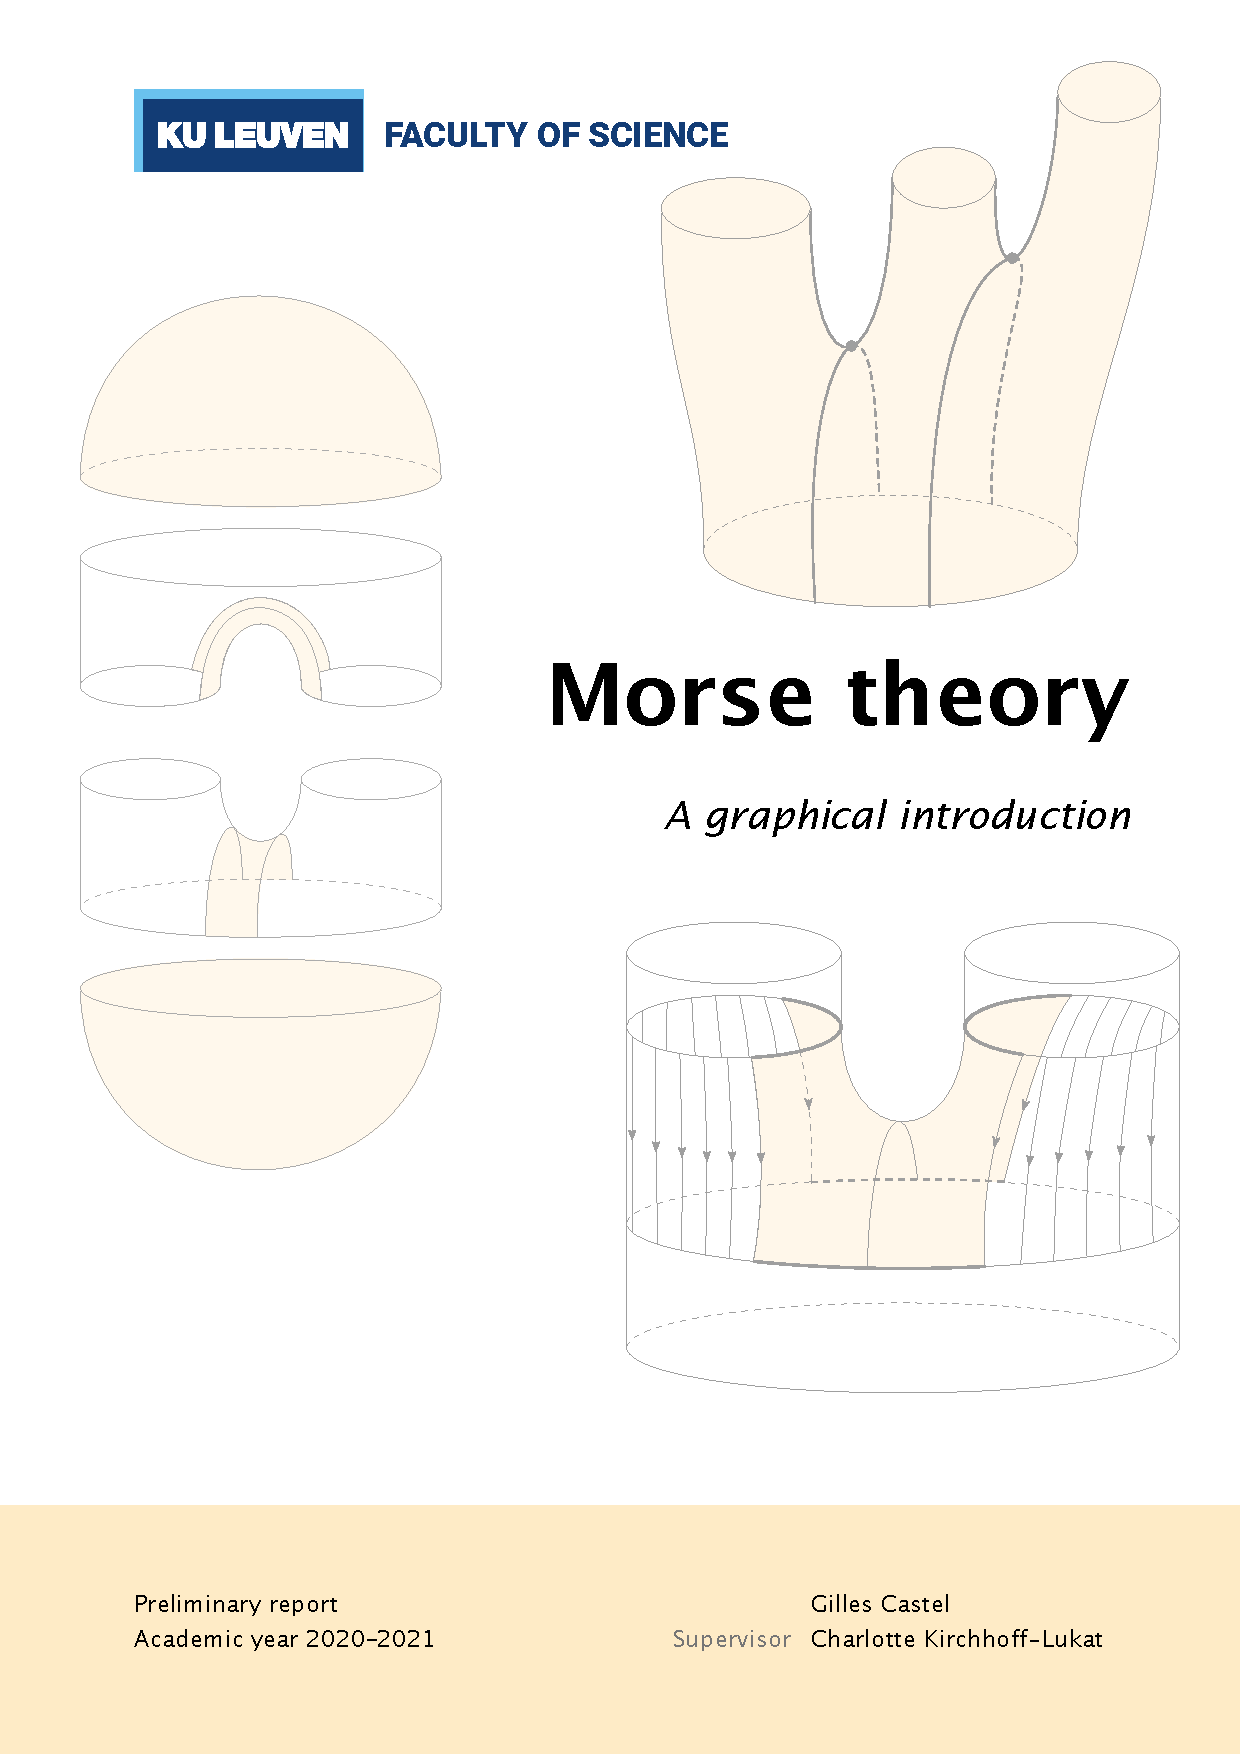
\includepdf[pages=-, fitpaper=true]{./frontmatter.pdf}
    \cleardoublepage
    \maketitle
    % \chapter*{Preface}
\label{ch:preface}
\addcontentsline{toc}{chapter}{\nameref{ch:preface}}

Lorem ipsum dolor sit amet, consetetur sadipscing elitr, sed diam nonumy eirmod
tempor invidunt ut labore et dolore magna aliquyam erat, sed diam voluptua. At
vero eos et accusam et justo duo dolores et ea rebum. Stet clita kasd gubergren,
no sea takimata sanctus est Lorem ipsum dolor sit amet.

    \chapter*{Summary}
\label{ch:summary}
\addcontentsline{toc}{chapter}{\nameref{ch:summary}}

Morse theory is the study of smooth functions from manifolds to $\R$ that satisfy a non-degeneracy condition. While these functions are some of the simplest things that live on manifolds, it turns out that they can provide great insight in the structure of manifolds.

\bigskip
In \textbf{Chapter \ref{chap:morse-theory}}, we talk about the basics of Morse theory.
We give several equivalent definitions of a Morse function and give some examples.
We also show that Morse functions give rise to so-called handle decompositions: there is a one to one correspondence between critical points of a Morse function and so-called handles, building blocks from which any manifold can be built.
We give some very concrete examples of handle decompositions in dimensions one, two and three.
We end the chapter by showing that any manifold admits (infinitely many) Morse functions.
Even more, we show that they are generic and stable, meaning that any function can be approximated by a Morse function and if we perturb a Morse function, it stays Morse.

\bigskip

\textbf{Chapter \ref{chap:stable-and-unstable-manifolds}} concerns the concept of stable and unstable manifolds.
They form a way of understanding interaction of handles.
For example, two handles are `independent' if the intersection of the associated stable and unstable manifolds is empty, allowing us to reorder them, as we prove in Theorem~\ref{thm:reordening}.
This idea leads to the existence of self-indexing Morse functions, asserting that we can always build a manifold by first attaching $0$-handles, then $1$-handles, $2$-handles, etcetera, in that order.
We end the chapter by proving a first cancellation theorem, stating that under certain circumstances, we can cancel pairs of critical points.

\bigskip
In \textbf{Chapter \ref{chap:morse-homology}}, we introduce Morse homology.
We first define the Morse complex $C_k(f)$ and the Morse differential $\partial_X$, which is based on counting the number of trajectories along the (pseudo-)gradient vector field $X$ between critical points of a Morse function $f$.
Morse homology $\HM f X$ is the homology associated to this complex.
As an illustration, we compute some examples in two and three dimensions.
The rest of the chapter covers three important theorems in Morse theory.
We prove that the Morse complex is actually a complex ($\partial_X^2 = 0$), that Morse homology is independent of the Morse function and gradient, and lastly that Morse homology is actually isomorphic to singular homology.
The proofs of these theorems are very geometrical in nature and their ideas have inspired many other theories.

\bigskip
\textbf{Chapter~\ref{chap:app-morse-homology}} discusses some applications of Morse homology.
While we now know that it is isomorphic to singular homology, and hence it enjoys all the properties of singular homology, it still can be illuminating to derive these facts directly from Morse homology.
For example, we can prove Poincaré duality by simply changing the Morse function $f \leadsto -f$, i.e.\ turning the manifold upside down.  This has the effect of $k$-handles becoming $n-k$-handles and flow lines reversing direction, from which the desired result follows rapidly.
We also discuss the Morse inequalities giving a lower bound for the number of critical points of a Morse function in terms of the singular homology of $M$:
 \[
     \# \Crit_k f \ge \operatorname{rank} H_k(M, \Z)
.\] 
We end the chapter by proving some related facts including a stronger version of the Morse inequalities.

\bigskip
In \textbf{Chapter~\ref{chap:h-cobord}}, we prove that under certain conditions, the Morse inequalities can be attained by some Morse function.
In other words, there always exists a Morse function such that $\# \Crit_k f = \operatorname{rank} H_k(M, \Z)$.
We prove this by considering an arbitrary Morse function,
and then cancelling pairs of critical points until the Morse inequalities have been reached.
To this purpose, this chapter mostly contains stronger cancellation results.
In Section~\ref{sec:minimality}, all these cancellation theorems come together and we prove the minimality of the Morse inequalities.
This has as an immediate corollary two of the most important theorems in differential topology: the $h$-cobordism theorem and the generalized Poincaré conjecture in dimension $n \ge 5$, stating that a homotopy sphere is a topological sphere.
To end this thesis, we also discuss some of the historical aspects of these theorems.

    \listofsymbols
    \tableofcontents
    \cleardoublepage
    \pagestyle{fancy}
    \renewcommand{\thepage}{\arabic{page}}
    \setcounter{page}{1}
    % \setcounter{chapter}{-1}
\chapter{Preliminaries}

\lipsum[1-10]

\newthought{Lorem ipsum dolor sit amet}, consetetur sadipscing elitr, sed diam nonumy eirmod
tempor invidunt ut labore et dolore magna aliquyam \sidenote{This is a side note!} erat, sed diam voluptua. At
vero eos et accusam et justo\sidecite{crandall2006prime}.
duo dolores et ea rebum. Stet clita kasd gubergren,
no sea takimata sanctus est Lorem ipsum dolor sit amet.

\begin{marginfigure}
    \centering
    \incfig[1]{test-figure}
    \caption{This is a test figure}
    \label{fig:test-figure}
\end{marginfigure}

\lipsum[1-5]

\begin{marginfigure}
    \centering
    \incfig[1]{test-figure}
    \caption{This is a test figure}
    \label{fig:test-figure}
\end{marginfigure}


\lipsum[6-10]

Bigger figure:


\begin{SCfigure}[b]
    \caption{This is a bigger figure. It shows some ellipses.}
    \incfig{bigger-figure}
    \label{fig:bigger-figure}
\end{SCfigure}
\lipsum[1-10]

This is a list:

\begin{itemize}
    \item Item 1
    \item Item 2
    \item Item 3
\end{itemize}

Large figure
\begin{figure*}
    \centering
    \incfig[1]{test-figure}
    \caption{This is a test figure. This is a really long caption!}
    \label{fig:test2-figure}
\end{figure*}

Theorem: 

\begin{theorem}[Sard's theorem]
    \lipsum[60]
\end{theorem}

    % \chapter*{Introduction}
\label{ch:introduction}

\addcontentsline{toc}{chapter}{\nameref{ch:introduction}}

    \setcounter{chapter}{-1}
\chapter{Preliminaries}

In this thesis, we assume the reader is familiar with basic concepts of differential geometry such as smooth manifolds, vector fields, flows, bundles, differential forms, et cetera.
In this chapter, we discuss some concepts that might be unfamiliar.

\section*{Differential Geometry}
\subsection*{Transversality}
The first concept we want to introduce is transversality.

\todo{Interesting source appendix of Schultens\sidecite{schultens2014introduction}}


% TODO: spell check in brackets in vim!
\begin{definition}[Transversality]
    Let $M$ be a manifold and $N_1, N_2$ be two submanifolds.
    Then $N_1$ intersects $N_2$ \emph{transversely} if and only if for all points of intersection $p \in N_1 \cap N_2$, we have
    $T_pM = T_pN_1 + T_p N_2$.
    We denote this by $ N_1 \tcap N_2$.\sidenotemark[0]
\end{definition}
\sidenotetext[0]{The notation is suggestive: the line $\cap$ intersects $|$ transversely $\tcap$.}
Note in particular that this depends on the ambient manifold $M$, and that if $N_1$ and $N_2$ do not intersect, their intersection is vacuously transverse.
We give some examples below.
\begin{figure}[H]
    \centering
    \sidecaption{
        Examples and non-examples of transverse intersections.
        Multiple configurations of two circles are shown: thrice with ambient manifold $\R^2$, and once embedded in $\R^3$.
    \label{fig:transversality-examples}
    }
    \incfig{transversality-examples}
\end{figure}
If the intersection of two manifolds $ N_1$ and $N_2$ is transverse, much more can be said about their intersection than in the general case.
In particular, as the following proposition states, we are guaranteed that $N_1 \tcap N_2$ is again a manifold, which as Figure~\ref{fig:intersection-of-manifolds-is-not-always-a-manifold} shows is not always true.
\begin{marginfigure}
    \centering
    \incfig{intersection-of-manifolds-is-not-always-a-manifold}
    \caption{Let $M = \R^2$ and let $N_1$ and $N_2$ be submanifolds as in the figure. Then $N_1$ and $N_2$ do not intersect transversely and their intersection is not a manifold: it is the union of a point and a closed interval.}
    \label{fig:intersection-of-manifolds-is-not-always-a-manifold}
\end{marginfigure}
\begin{prop}
    Let $M$ be a manifold and $N_1, N_2$ be two submanifolds. If $ N_1 \tcap N_2$, then $ N_1 \tcap N_2$ is again a manifold and 
    \[
        \codim (N_1 \tcap N_2) = \codim N_1 + \codim N_2
    ,\] 
    where the codimensions are to be taken with respect to $M$, by which we mean $\codim N_i = \dim M - \dim N_i$.
    Moreover, $T(N_1\tcap N_2) = TN_1 \tcap TN_2$.
\label{prop:transverse-codimensions-add}
\end{prop}
\begin{proof}
    As this is a local statement, we prove it for $M = \R^{m}$.
    We may assume that $N_1 = f_1^{-1}(0)$ and $ N_2 = f_2^{-1}(0)$ where $f_i$ are submersions from $\R^{m}$ to $\R^{n_i}$, where $n_i$ is the codimension of $N_i$.
    % i.e. $(f_i)_*$ has full rank everywhere.
    Then we can also consider $F= (f_1, f_2): \R^{m} \to  \R^{n_1} \times \R^{n_2}$.
    Notice that $ N_1 \cap N_2 = F^{-1}(0)$.
    Then
    \begin{align*}
        \dim N_1 \cap  N_2 &= \dim \Ker d_0F\\
                           &= \dim(\Ker d_0 f_1 \cap \Ker d_0 f_2)\\
                           &= \dim \Ker d_0 f_1 + \dim \Ker d_0 f_2 - \dim (\Ker d_0 f_1 + \Ker d_0 f_2)\\
                           &= (m - n_1) + (m - n_2) - m\\
                           &= m - (n_1 + n_2)
    .\end{align*} 
    This also shows that $T_p(N_1 \tcap N_2) = T_pN_1 \tcap T_pN_2$ and that $ N_1 \tcap N_2$ is a manifold, which is not always the case when the intersection is not transverse.
\end{proof}
\begin{marginfigure}[-5cm]
    \centering
    \incfig{codimensions-transverse}
    \caption{When $N_1 \tcap N_2$, the codimension of the intersection is the sum of their codimensions. By using the implicit function theorem, we straighten the situation.}
    \label{fig:codimensions-transverse}
\end{marginfigure}

An interesting property of transversality is that it is both \emph{generic} and \emph{stable}.
By generic we mean that any two manifolds intersecting can be made intersecting transversely by perturbing one of the manifolds.
Stability on the other hand means that when we perturbate a transverse intersection, it stays transverse.
At the core of the proof of stability and genericness of transversality lies the theorem of Sard:
% In morse rigorous terms, we have the following:
% \begin{definition}[Stable]
%     A property $P$ is stable for a class $C$ of maps $f:M \to  N$ if for all $f \in C$ that satisfy $P$, we have that there any homotopy  $f_t$ with  $f_0 = f$ there exists an $\epsilon>0$ such that  $f_t$ satisfies $P$ for each  $t < \epsilon$.
% \end{definition}
% \begin{definition}[Generic]
%     A property $P$ is generic for a class  $C$ of maps $f: M \to  N$ if the set of 
% \end{definition}
\begin{theorem}[Sard's theorem]
    Let $f: M \to  N$ be a $\Cinfty$ map. Then the set of critical values of  $f$ has measure zero in $N$.
\end{theorem}
Note in particular that it is the set of critical \emph{values} that has measure zero, not the set of critical points. 

% \begin{definition}[Isotopy]
%     Two embeddings $f_0, f_1: M \to  N$ are \emph{isotopic} if there is a continuous map $H: M \times  [0, 1] \to  N$ such that $H(x, 0) = f_0$ and $H(x, 1) = f_1(x)$ for all $x \in M$ and such that for all $t \in [0, 1]$, the map $f_t$ defined by $H(\cdot , t)$ is an embedding. The map $H$ is called an \emph{isotopy between} $f_0$ and $f_1$.

%     Two submanifolds $S_0, S_1$ of $M$ are \emph{isotopic} if their inclusion maps are isotopic.
% \end{definition}
% \sidenotetext{\fullcite[23]{schultens2014introduction}}


\subsection*{Intersection number}

\begin{marginfigure}
    \centering
    \incfig{intersection-number}
    \caption{
        The intersection number is defined by comparing the orientation of $N$ with the coorientation of $N'$ at the points of transverse intersection.
        In this case, the ambient manifold $M = \R^2$, $N = (0,1)$ and $N' = S^1$ and $N' \cdot N = -1 + 1 = 0$.
    }
    \label{fig:intersection-number}
\end{marginfigure}
\begin{definition}[Intersection number]
    Let $N$ and  $N'$ be $r$- and  $s$- dimensional submanifolds of an $(r+s)$-dimensional manifold $M$.
    Suppose $N$ is oriented, $N'$ is cooriented and their intersection is transverse.
    Let $p \in  N \tcap N'$.
    Then $T_p N$ is oriented both by the orientation of  $N$ and the coorientation of  $N'$.
    If these orientations match, we define the intersection number at $p$ to be $+1$, otherwise we define it to be $-1$.
    The intersection number  $N' \cdot N$ is then defined as the sum of all the intersection numbers at the points in $N \tcap N'$.
\end{definition}
\begin{remark}
    If we change the order, the intersection number might change sign: $N \cdot N' =  \pm N' \cdot N$.
\end{remark}
\begin{prop}
    The intersection number $N \cdot N'$ does not change under ambient isotopies of $N$ or $N'$.
    In particular, we can define the intersection number of two manifolds that do not intersect transversely.
\end{prop}
\begin{proof}
    See `Differential Manifolds'\sidecite[p.~70]{kosinski2013differential}.
\end{proof}
\begin{eg}
    Consider the intersection of $M  = S^{1}$ and an interval embedded in $\R^2$. Consider the orientation of $M$ and coorientation of $M$ as defined in Figure~\ref{fig:intersection-number}. Then $M' \cdot M  = -1 + 1 = 0$.
    It is also clear that the intersection number does not change under isotopies of the manifolds.
\end{eg}


\section*{Homological Algebra}
In this section, we will assume that the reader is familiar with modules over a ring $R$. If not, they can mentally substitute each occurence of `module' by `vector space'.

\begin{definition}[Chain complex]
    A chain complex of $R$-modules is a sequence $M_\bul$ of the form
    \[
    \cdots \to  M_2 \xrightarrow{d_2}  M_1 \xrightarrow{d_1} M_0 \xrightarrow{d_0} M_{-1} \xrightarrow{d_{-1}}   M_{-2} \to  \cdots
    \] 
    where each term $M_i$ is an $R$-module and $d_i: M_i \to  M_{i-1}$ is an $R$-module homomorphism such that $d_{i-1}  \circ  d_i = 0$  for all $i \in \Z$.
\end{definition}
We often suppress the indices of the maps $d_i$ and the last condition becomes then  $d^2 = 0$.

\begin{marginfigure}
    \centering
    \incfig{homology-definition}
    \caption{Homology measure exactness of a chain complex.}
    \label{fig:homology-definition}
\end{marginfigure}

\begin{definition}[Homology]
    Let $M_\bul$ be a chain complex of  $R$-modules. The $i$-th homology of $M_\bul$ is
     \[
         H_i(M_\bul) = \frac{\Ker d_i}{\Im d_{i+1}}
    .\] 
    This is well defined because $\Im(d_{i+1}) \subset \Ker (d_i)$.
\end{definition}
It is clear that this measure the exactness of the sequence. Indeed, if the sequence is exact, i.e. $\Im d_{i+1} = \Ker d_i$, then $H_i(M_\bul) = 0$.


\begin{definition}[Chain map]
    A chain map $f_\bul: M_\bul \to  N_\bul$ is a collection of $R$-module homomorphisms which makes the following diagram commute:
    \[
        \begin{tikzcd}
            \cdots  \arrow[r, ""]&
            M_{i+1} \arrow[r, "d_{i+1}^{M}"] \arrow[d, "f_{i+1}"]&
            M_{i} \arrow[r, "d_{i}^{M}"] \arrow[d, "f_i"]&
            M_{i-1} \arrow[r, ""] \arrow[d, "f_{i-1}"]&
            \cdots \\
            \cdots  \arrow[r, ""]&
            N_{i+1} \arrow[r, "d_{i+1}^{N}"] &
            N_{i} \arrow[r, "d_{i}^{N}"] &
            N_{i-1} \arrow[r, ""] &
            \cdots \\
        \end{tikzcd}
    \]
    In other words, suppressing indices, $f  \circ  d^{M} = d^{N}  \circ f$.
\end{definition}

It is easy to check that chain maps induce a map on the level on homology which we denote by $H_i(f_\bul): H_i(M_\bul) \to  H_i(N_\bul)$, proving that $H_i$ is a functor. 

The following is a useful criterion for determining whether two chain maps induce the same maps on the level on homology.
\begin{definition}[Chain homotopic]
    Let $f_\bul, g_\bul$ be chain maps between  $M_\bul$ and $N_\bul$.
    A chain homotopy from  $f_\bul$ to  $g_\bul$ is a collection of  $R$-module homomorphisms $h_i: M_i \to  N_{i+1}$ such that $g_i - f_i = d^{N}_{i+1}  \circ  h_i + h_{i-1}  \circ  d_i^{M}$ for all $i$.
    If such a map exists, we say that $f_\bul$ and  $g_\bul$ are chain homotopic.
    \[
        \begin{tikzcd}[column sep=3em, row sep=3em]
            \cdots  \arrow[r, ""]&
            M_{i+1} \arrow[r, "d_{i+1}^{M}"] \arrow[d, "f_{i+1}"', shift right=2pt] \arrow[d, "g_{i+1}", shift left=2pt]&
            M_{i} \arrow[r, "d_{i}^{M}"] \arrow[d, "f_i"', shift right=2pt] \arrow[d, "g_{i}", shift left=2pt] \arrow[dl, "h_i"', dashed]&
            M_{i-1} \arrow[r, ""] \arrow[d, "f_{i-1}"', shift right=2pt]\arrow[d, "g_{i-1}", shift left=2pt] \arrow[dl, "h_{i-1}"', dashed]&
            \cdots \\
            \cdots  \arrow[r, ""]&
            N_{i+1} \arrow[r, "d_{i+1}^{N}"] &
            N_{i} \arrow[r, "d_{i}^{N}"] &
            N_{i-1} \arrow[r, ""] &
            \cdots \\
        \end{tikzcd}
    \]
    Suppressing indices, this becomes $g - f = dh + hd$.
\end{definition}
\begin{prop}
    Let $f_\bul, g_\bul$ be two chain homotopic chain maps from $M_\bul$ to $N_\bul$. 
    Then $H_i(f_\bul) = H_i(f_\bul)$, i.e.\ the maps induced on the level of homology are identical.
\end{prop}
\begin{proof}
    Let $h_i$ be a chain homotopy between  $f_\bul$ and  $g_\bul$.
    Let $x \in \Ker(d_i^{M})$.
    Then, suppressing indices,
    \begin{align*}
        g(x) + \Im(d^{N}) &= f(x) + (h  \circ  d^{M})(x) + (d^{N}  \circ h)(x)  + \Im(d^{N})\\
                          &= f(x) + h(0) + \Im(d^{N})\\
                        &= f(x) + \Im(d^{N}).
    \end{align*} 
\end{proof}

\todo{
    \begin{itemize}
        \item Example of singular homology
        \item Relative homology
        \item Cohomology via hom functor (exact if field)
        \item Mayer vietoris
    \end{itemize}
}

\todo{Add source. Above: commutative algebra}
\begin{definition}[Tensor product of complexes]
    Let $C_\bul$ and  $D_\bul$ be two complexes over field. Their tensor product is defined as
     \[
         (C \otimes D)_k = \bigoplus_{i+j = k} C_i \otimes D_j
    ,\] 
    with boundary operator $\partial_C \otimes 1 + 1 \otimes\partial_D$.
\end{definition}
\todo{Add picture}
\begin{prop}
    Let $C_\bul$ and  $D_\bul$ be complexes over a field.
    The homology of the tensor product complex is the tensor product of the homologies:
    \[
        H_\star(C_\bul \otimes D_\bul) = H_\star(C_\bul) \otimes H_\star(D_\bul)
    .\] 
    \label{prop:hom-tensor-is-tensor-hom}
\end{prop}
\begin{proof}
    Omitted.
\end{proof}
\begin{remark}
    This result is only true when we are working over a field, i.e.\ in the context of vector spaces.
\end{remark}
\todo{Add source (Audin)}


\begin{definition}[Fundamental group (TODO)]

\end{definition}
\begin{definition}
    Seifert van kampen
\end{definition}

    \chapter{Morse theory}

When studying manifolds is often proves useful to study simple structures that live on manifolds. For example, studying differential forms gives rise to the de Rham cohomology, which tells us something about the global structure of the manifold. In this thesis, we study functions from the manifold to $\R$, some of the most simple functions you can imagine. You can think of them as projections  to one dimension.
While these projections seem to lose much information, we will see that they actually can provide great insight in the structure of the manifold itself.

We will not consider arbitrary maps $M \to \R$, but rather maps that have nice behaviour at their critical points. Let us first recall what a critical point is.

\begin{definition}[Critical point]
    Let $M$ and $N$ be a manifolds and  $f$ a map from $M$ to $N$.
    The critical points of $f$ are
    \[
    \Crit f = \{p \in M  \mid \text{$df_p$ is not surjective}\} 
    .\] 
    In particular, if $N = \R$ we have that
    \[
    \Crit f = \{ p \in M  \mid  df_p = 0\} 
    .\] 
\end{definition}
The maps we are to consider are called `Morse functions' and are defined as follows.
\begin{definition}[Morse function]
    Let $M$ be a manifold. A function $f: M \to  \R$ a \emph{Morse function} if for all critical points $p$, there exists a chart centred around $p$ such that $f$ is locally given by
    \[
        f(x) = f(p) -x_1^2 - \cdots - x_k^2 + x_{k+1}^2 + \cdots + x_n^2
    .\] 
    We call such a chart a \emph{Morse chart} and we call $k$ the index of $p$, which we also denote with $\Ind p$.
    
\end{definition}
Intuitively, the index of a critical point $p$ is ``the number of downward directions''.
Let us first give some examples.
\begin{marginfigure}
    \centering
    \incfig{examples-of-morse-functions}
    \caption{Example of a Morse function on the torus. At each critical point, the index $k$, the number of downward directions is indicated. }
    \label{fig:examples-of-morse-functions}
\end{marginfigure}
\begin{eg}
    Let $M$ be the torus  $T^2$ embedded in $\R^3$ as illustrated in \cref{fig:examples-of-morse-functions}.
    Then the height function $h: T^2 \to  \R$ which is the projection on the $z$-axis is a smooth map with four critical points:
    \begin{itemize}
        \item A minimum $m$, where $h(x) = h(m) + x_1^2 + x_2^2$.
        \item Two saddle points $s_1, s_2$ where $h(x) = h(s_i) + x_1^2 - x_2^2$.
        \item A maximum $p$ where $h(x) = h(p) - x_1^2 - x_2^2$.
    \end{itemize}
\end{eg}

\begin{eg}
    Let $M = \R^2$ and $f: \R^2 \to  \R: (x, y) \mapsto  x^2$.
    Then all points $(0, y)$ for  $y \in \R$ are critical points of this function.
    In particular, $(0, 0)$ is a critical point, but $f$ is clearly not Morse.
\end{eg}
\begin{marginfigure}
    \centering
    \incfig{non-example-of-morse-function}
    \caption{}
    \label{fig:non-example-of-morse-function}
\end{marginfigure}
\begin{marginfigure}
    \centering
    \incfig{non-examples-of-morse-functions}
    \caption{An example of a function that is not Morse: $f: \R \to  \R: x \mapsto  x^3$.
        Small perturbations of $f$ are Morse.
    }
    \label{fig:non-examples-of-morse-functions}
\end{marginfigure}
\begin{eg}
    Let $M = \R$ and $f : \R \to  \R: x \mapsto x^3$.
    Then $x = 0$ is a critical point, but $f$ is not Morse.
    Note however that if we add a small perturbation to $f$, say $g_t: x\mapsto x^3+ tx$, then for small non-zero $t$, $g$ is Morse. For $t < 0$, $g_t$  has two critical points: one of index $1$ and one of index $0$.
    If $t > 0$,  $g_t$ has no critical points.
\end{eg}

Note that this last case where $f$ has no critical points cannot happen if $M$ is compact.
Indeed, any function attains it maximum and minimum on a compact manifold, so we have at least two critical points.
On the other hand, the number of critical points is at most finite.
Indeed, the definition of a Morse function implies that critical points are isolated, which on a compact manifold implies that their number is finite.
This also immediately rules out the situation we had in the other example, where the set of critical points was a straight line.

\section{Handle decompositions}
\todo{Introduction}

\todo{Check definition Milnor $h$-cobordism and fix definition Morse function}
\begin{definition}
A cobordism between two compact manifolds $M_1$ and $M_2$ is a compact manifold $M$  with boundary $\partial M = M_1 \sqcup M_2$.
\end{definition}


The term `cobordism' comes from the fact that $M_1 \sqcup M_2$ are the boundary of $M$, so you can think of $M$ as the `co-boundary' of $M_1$ and $M_2$.
Cobordisms are an interesting topic in its own right.
For example, they define an equivalence relation on all compact manifolds of same dimension. Two manifolds $ M_1$ and $M_2$ are then said to be equivalent (cobordant) if there exists a cobordism $M$ connecting the two.
This equivalence relation is coarser than diffeomorphism and is generally easier to study.
Cobordisms also form a category where the objects are manifolds and the arrows are cobordisms.

We have illustrated some examples below.
Note that we may also take $M_1$ or $M_2 = \O$.
In particular, any closed manifold is a cobordism from $\O$ to $\O$.
\begin{figure}[H]
    \centering
    \sidecaption{Some examples of cobordisms. 
        When the height function has critical points, the topology changes.
    \label{fig:examples-of-cobordisms} }
    \incfig{examples-of-cobordisms}
\end{figure}

When we consider the height function $f: M \to  [0, 1]$ on these examples,
we observe that the topology of the bottom is different than that of the top if the height function has critical points.
This is indeed in general true.
If $f$ is a Morse function (which is the case in our examples), it will turn out we can very concretely describe \emph{how} this topology changes.
This will give rise to handle decompositions.

\newthought{Let us first consider} the case where $f: M \to [0, 1]$ has no critical points. 

\begin{prop}
    Suppose $M$ is a cobordism from $M_0$ to $ M_1$ and $f : X \to [0, 1] $ such that $M_0 = f^{-1}(0)$ and $M_1 = f^{-1}(1)$.
    Suppose $f$ has no critical points. Then $X$ is diffeomorphic to $[0, 1] \times  M_0$.
\end{prop}
\begin{proof}
    \todo{Check proof $h$-cobordism milnor}
    \begin{marginfigure}
        \centering
        \incfig{proof-of-cobordism-without-critical-points}
        \caption{TODO proof of cobordism without critical points}
        \label{fig:proof-of-cobordism-without-critical-points}
    \end{marginfigure}
    Consider a Riemannian metric $\left<\cdot ,\cdot  \right>$ on $M$.
    Because  $f$ has no critical points, the vector field $W = (df)^{\sharp}$ never vanishes.
    Consider the normalized vector field
    \[
    V = \frac{1}{\left<W, W \right>} W
    .\] 
    Then $df(V) = \frac{1}{\left<W, W \right>} df(W) = 1$.
    Consider
    \begin{align*}
        \phi: [0, 1] \times M_0&\longrightarrow M \\
        (t, p) &\longmapsto \theta_V^{t}(p)
    ,\end{align*}
    where $\theta_V^{t}$ is the flow along $V$.
    Then $f(\phi(t, p)) = t$ for all $p \in M_0$, as $df(V) = 1$.
    The map $\phi$ is injective because of the uniqueness of flows, and surjective because given a point $p$ in $M$, we can always flow back along $V$ for a time $t$ to find a $p_0 \in M_0$ which then satisfy $\phi(t, p_0) = p$. 
    This also proves that $\phi$ is a diffeomorphism.
\end{proof}

\todo{This is sometimes used to prove that two things are diffeomorphic!}

\todo{Corollary: collar and bicollar theorem. Milnor $h$-coboridsm.}
\todo{Corollary: we can glue two cobordisms together and get a manifold un a unique way. Milnor $h$-coboridsm.}

In the case in which $f$ does have a critical point, the previous proof fails because $df = 0$, so $\grad f = (df)^{\sharp}$ vanishes at some point.


\newthought{Let us now investigate} the situation when a Morse function $f$ does have a single critical point, say $p$ and assume $f(p) = 0$.
Then we know $f$ is locally of the following form:
\[
    f(x_1, \ldots, x_n) = - x_1^2 - \cdots - x_k^2 + x_{k+1}^2 + \cdots + x_n^2
.\] 
In Figure~\ref{fig:morse-chart}, we have plotted the first $k$ variables (the `downward directions') on the horizontal axis, and the last $n-k$ variables on the vertical axis.
Then the level set $f^{-1}(0)$ is given by
\[
x_1^2 + \cdots + x_k^2 = x_{k+1} ^2 + \cdots + x_n^2
,\] 
which consists of the two crossing lines in the figure, corresponding to the crossing part of the figure-eight on the right.
Level sets of values slightly above an below $0$ look locally like hyperbolas on our figure, but remembering that that the axes consist of multiple dimensions, we should call them hyperboloids.

\todo{Add figure movie: two hyperbolas switching, hyperboloids, one handle in three dimensions that joins, \ldots}
\begin{figure}[H]
    \centering
    \sidecaption{TODO: morse chart 
    \label{fig:morse-chart}}
\incfig{morse-chart}
\end{figure}

To contain the behaviour of the critical point, it is useful to cut out the area bounded by the level sets $f = \pm \epsilon$ in order to make it compact.\todo{wording}.
A natural way to do this, is to cut along gradient flow lines of $f$ (Figure~\ref{fig:morse-chart-flow-lines} and \ref{fig:morse-chart-zoomed-in}), by which we mean gradient lines for the standard metric on $\R^{n}$.\sidenote{More explicitly, if $f$ is Morse, we know that locally around a critical point $p$, $f$ is given by
    \begin{align*}
        f(x_1, \ldots, x_n) &= f(p) - x_1^2 - \cdots - x_k^2\\
                            & \qquad + x_{k+1}^2 + \cdots + x_n^2
    .\end{align*} 
    Then the gradient of $f$ w.r.t.\ the standard metric on $\R^n$ is
    \begin{align*}
        \grad f &= - 2 x_1 \partial_{1} - \cdots - 2 x_k \partial_{k}\\
                & \qquad + 2 x_{k+1} \partial_{k+1} + \cdots + 2 x_n \partial_{n},
    \end{align*}
    where $\partial_i = \partial_{x_i}$.
}
\begin{marginfigure}
    \centering
    \incfig{morse-chart-flow-lines}
    \caption{TODO morse-chart-flow-lines}
    \label{fig:morse-chart-flow-lines}
\end{marginfigure}
In Figure~\ref{fig:morse-chart-zoomed-in}, the cut out area is coloured in yellow.
The advantage of cutting along gradient flow lines, is that we have split up the cobordism in three parts which we understand well.
\begin{itemize}
    \item[\circled{A}] The part below $-\epsilon$ and the part above $\epsilon$ have a product structure, because we assumed the only critical value was $0$.
    \item[\circled{B}] The part of $M$ that lies between $-\epsilon$  and $\epsilon$ without $\circled{H}$ also has a product structure.
        To see this, extend the metric on $\circled{H}$ to the whole manifold. Then, because $f$ has no critical values outside $\circled{H}$, we can flow along gradient lines giving us product structure.
        This is why we cut in this way: we want the boundary of this region to consist of gradient lines, or the proof would fail.

        Riemannian metrics are an extension of standard metrics around critical points are called adapted Riemannian metrics.
        Using a partition of unity argument, one can show any manifold admits such metrics.
        \begin{definition}[Adapted Riemannian metric]
            A Riemannian  metric is called \emph{adapted} to a Morse function $f$ if near all its critical points $p \in \Crit f$, the metric is locally, in each Morse chart given by
            \[
            \left<
            (x_1, \ldots, x_n), 
            (y_1, \ldots, y_n)
            \right> = \sum x_i y_i
            .\] 
        \end{definition}
        \todo{Convention: positive or negative gradient? Also in the figures!}
        In most cases, we often forget about the metric itself and simply consider vector fields which are gradient-like.

        \begin{definition}[Pseudo-gradient]
            Let $f: M \to  \R$ be a Morse function on a manifold $M$. A pseudo-gradient is a vector field $X$ such that
            \begin{itemize}
                \item $df(X) \le 0$ and $df(X) = 0$ only at critical points
                \item $X$ coincides in Morse charts with the usual negative gradient for the standard metric on $\R^{n}$.
            \end{itemize}
        \end{definition}




    \item[\circled{H}]  The yellow part is what we call a \emph{handle of index $k$}, and is homeomorphic to $\disk{k} \times \disk{n-k}$.
        This is the only non-trivial part of our cobordism.
        We call the bottom part of the border the \emph{attachment region}, i.e. $S^{k-1} \times \disk{n-k}$.
\end{itemize}
\begin{marginfigure}
    \centering
    \incfig{morse-chart-zoomed-in}
    \caption{morse-chart-zoomed-in TODO}
    \label{fig:morse-chart-zoomed-in}
\end{marginfigure}






\newthought{If a Morse function} on a cobordism has multiple critical points, then we can always assume that the critical values are distinct and isolated.
We can do this by adding a small perturbation to $f$.\todo{prove this}.
Then we can split up the cobordism in parts having only one or zero critical points, and decompose each part in products and handles like before.

As any closed manifold can be viewed as a cobordism from $\O$ to $\O$, we have proved the following

\begin{theorem}
    Any closed manifold has a handle decomposition.
\end{theorem}

Before discussing some examples, let us first discus some of the different ways to look at handles.
\todo{Add subtleties about corners, \ldots
Thickened up intervals.
Instead of having morse function and decomposing, you can also ask question how you can build a manifold?

Embed attachment region in the manifold you already have.}


Let us now look at examples in low dimensions.
\subsection{Handles in low dimensions}
In this section, we will consider some examples of handle decompositions in dimension one, two and three.

\newthought{Handles in dimension one} are the most simple ones. We only have two types:

\begin{description}
    \item[$0$-handle] $\disk0 \times \disk{1} = [-1, 1]$, with attachment region $\O$. \todo{These should probably be open intervals. Notation is inconstent\ldots} \hfill \minifig{1cm}{handle-1-0} 
        
    \item[$1$-handle]   $\disk{1} \times  \disk{0} = [-1, 1]$ with attachment region $S^{0} = \{-1, 1\}$.  \hfill \minifig{1cm}{handle-1-1}
\end{description}

\begin{eg}
    In Figure~\ref{fig:one-dimensional-handle-decomposition-examples}, two handle decompositions of $S^{1}$ are illustrated.
    The first one is based on the height function $f$ when embedding $S^{1}$ in $\R^2$.
    For the second decomposition, $g$ is again defined as a height function, but this time we embedded $S^{1}$ in $ \R^2$ in a non-standard way.
    This way, we get two different handle decompositions of the same manifold.
\end{eg}
\begin{figure}[H]
    \centering
    \sidecaption{Two handle decompositions of $S^{1}$.
    \label{fig:one-dimensional-handle-decomposition-examples}}
    \incfig{one-dimensional-handle-decomposition-examples}
\end{figure}
This example illustrates that handle decompositions are not unique.
However, we can construct an isotopy from the second to the first embedding that cancels the two critical points.
Interestingly, the height function is Morse for all $t$, except at the exact moment when the cancellation happens.
A local model for this is $t\mapsto x^3 + tx$ as in Figure~\ref{fig:non-examples-of-morse-functions}.
\begin{figure}[H]
    \centering
    \sidecaption{TODO isotopy between circle and other circle
    \label{fig:isotopy-between-circle-and-other-circle}}
    \incfig{isotopy-between-circle-and-other-circle}
\end{figure}


\paragraph{Handles in dimension two}
In dimension two, things get more interesting.
We have three types of handles:
\todo{Mention somewhere homology group changes when adding handles. But handle decomposition is not unique, if we could mod out these critical points which can cancel, then it is unique? Giving rise to Morse complex.}

\begin{description}
    \item[$0$-handle] $\disk{0} \times \disk{2}$ with attachment region $\O$. \hfill \minifig{1cm}{handle-2-0}
    \item[$1$-handle] $\disk{1} \times \disk{1}$ with attachment region $\disk1 \times S^{0}$. \hfill\minifig{1cm}{handle-2-1}
    \item[$2$-handle] $\disk{2} \times \disk{0}$ with attachment region $\disk{0} \times S^1$. \hfill\minifig{1cm}{handle-2-2}
\end{description}

\begin{eg}[Handle decomposition of the torus]
    Consider the height function on the torus embedded in $\R^3$. This Morse function gives rise to the handle decomposition in Figure~\ref{fig:handles-in-dimension-two-torus-decomposition}: a $0$-handle, two $1$-handles and one $2$-handle.
\end{eg}

\begin{marginfigure}
    \centering
    \incfig{handles-in-dimension-two-torus-decomposition}
    \caption{TODO handles in dimension two torus decomposition}
    \label{fig:handles-in-dimension-two-torus-decomposition}
\end{marginfigure}

\begin{eg}[The `other sphere']
    In Figure~\ref{fig:handles-in-dimension-two-other-sphere}, an embedding of $S^2$ in $\R^3$ is given, and we again consider the height function.
    This function is Morse, and gives rise to a handle decomposition with a $0$-handle, a $1$-handle and two $2$-handles.
\end{eg}
\begin{marginfigure}
    \centering
    \incfig{handles-in-dimension-two-other-sphere}
    \caption{TODO handles in dimension two other sphere}
    \label{fig:handles-in-dimension-two-other-sphere}
\end{marginfigure}



\paragraph{Handles in dimension three}

\todo{Mention that sometimes you cannot attach handle before other one. When \emph{is} it possible? Hint to descending manifold, \ldots}

\begin{description}
    \item[$0$-handle] $ \disk0 \times \disk{3}$ with attachment region $\O$ 
        \hfill\minifig{1cm}{handle-3-0}
    \item[$1$-handle] $ \disk1 \times \disk{2}$ with attachment region $ \disk2 \times S^{0}$
        \hfill\minifig{1cm}{handle-3-1}
    \item[$2$-handle] $ \disk2 \times \disk{1}$ with attachment region $ \disk1 \times S^1$
        \hfill\minifig{1cm}{handle-3-2}
    \item[$3$-handle] $ \disk3 \times \disk{0}$ with attachment region $S^{2}$
        \hfill\minifig{1cm}{handle-3-3}
\end{description}

Drawing three-dimensional handle decompositions is a bit harder. Most of the times we suppress the $0$-handle, and also the $3$-handle is not drawn. If a $3$-handle is to be attached, we usually write ``$\cup $ $3$-handle''

\begin{eg}[Handle decomposition of $S^{3}$]
    Consider $S^{3} \subset \R^{4}$ and the height function $f$, the projection on the last coordinate.
    Then $f$ has two critical points: $(0, 0, 0, \pm 1)$ of index $0$ and $3$.
    Then handle decomposition is then a $0$-handle ($\disk{3}$) glued to a $3$-handle (which is also diffeomorphic to $\disk{3}$).
\end{eg}

\begin{eg}[Handle decomposition of $ S^1\times S^{2}$]
    An example of a handle decomposition of $S^{1} \times S^{2}$ is illustrated in Figure~\ref{fig:handles-in-dimension-three-s1-x-s2}.
    The construction starts with a $0$-handle, which is just a three dimensional ball.
    Then we glue on a $2$-handle.
    The resulting manifold is then a thickened-up \todo{spelling}  two sphere, $I \times S^{2}$.
    Then we add a $1$-handle connecting the inside to the outside and we cap of with a $3$-handle, which has the effect of identifying the end points of $I$, i.e. this transforms  $I \times S^{2}$ into $ S^1 \times S^{2}$.
\end{eg}
\begin{marginfigure}
    \centering
    \incfig{handles-in-dimension-three-s1-x-s2}
    \caption{TODO: Handle decomposition of $S^{1} \times S^{2}$}
    \label{fig:handles-in-dimension-three-s1-x-s2}
\end{marginfigure}

\begin{eg}
    \todo{Example of a $1$ and $2$-handle that collapse. }
\end{eg}
\begin{eg}[$T^{3} = S^{1} \times S^{1} \times S^{2}$]
    \label{eg:handle-decomposition-three-torus}
    To find a handle decomposition of $T^3$, identify $T^{3}$ with $\R^3 / \Z^{3}$ and consider
    \begin{align*}
        f: T^{3} &\longrightarrow \R \\
        (x, y, z) &\longmapsto \cos (2 \pi x) + \cos ( 2 \pi y) + \cos(2 \pi z)
    .\end{align*}
    Then
    \[
        df = -2\pi (\sin (2 \pi x) dx+ \sin ( 2 \pi y) dy + \sin(2 \pi z) dz)
    ,\] 
    so critical points are all $(x, y, z) \in \R^3 / \Z^3$ for which  $x, y, z \in \left\{0, \frac{1}{2}\right\}$.
    In total we have $8$ critical points, and they all are non-degenerate, because the Hessian of $f$
    \[
        H_{(x, y, z)} f = - (2 \pi)^2  (\cos (2 \pi x) dx^2 + \cos ( 2 \pi y) dy^2 + \cos(2 \pi z) dz^2)
    \] 
    is non-degenerate at each of the critical points.
    \todo{We need to discuss non-degeneracy and hessian before this!}

    \begin{tabular}{ccccr}
        $x$ & $y$ & $z$ & $f(x, y, z)$ &  Index\\ \hline
        $0$ & $0$ & $0$ & $todo$ & $3$ \\
        $0$ & $0$ & $\frac{1}{2}$ & $todo$ & $2$ \\
        $0$ & $\frac{1}{2}$ & $0$ & $todo$ & $2$ \\
        $0$ & $\frac{1}{2}$ & $\frac{1}{2}$ & $todo$ & $1$ \\
        $\frac{1}{2}$ & $0$ & $0$ & $todo$ & $2$ \\
        $\frac{1}{2}$ & $0$ & $\frac{1}{2}$ & $todo$ & $1$ \\
        $\frac{1}{2}$ & $\frac{1}{2}$ & $0$ & $todo$ & $1$ \\
        $\frac{1}{2}$ & $\frac{1}{2}$ & $\frac{1}{2}$ & $todo$ & $0$ \\
    \end{tabular}

    So we can decompose $T^3$ in one $0$-handle, three $1$-handles, three $2$-handles and one $3$-handle.

    A natural question that arises is: `Can we build $T^{3}$ using less handles'?
    \todo{Mention that values of critical points are not distinct}


    \todo{Explain and make full page width}
    \begin{figure}[H]
    \centering
    \incfig{three-torus-handle-decomposition}
    \caption{TODO three torus handle decomposition}
    \label{fig:three-torus-handle-decomposition}
\end{figure}
\end{eg}



\todo{Why can we cap off with a top-handle?}

\section{Coordinate-free definition of a Morse function}


The attentive reader will have noticed that the definition of the index of a critical point could possibly not be well defined.
To show that it is and that $\Ind p$ does not depend on the choice of coordinates, we will will give a coordinate-free definition. For this, we first need to define the Hessian at a critical point.

\begin{definition}
    Let $M$ be a manifold and $f: M \to  \R$ a function.
    Let $p$ be a critical point of $f$.
    Then we define the Hessian $H_p$ to be the bilinear form
    \begin{align*}
        H_p: T_pM \times T_pM &\longrightarrow  \R\\
        (X, Y) &\longmapsto X (\tilde{Y} f)|_p
    ,\end{align*} 
    where $\tilde{Y}$ is a local extension of $Y$ around $p$.
\end{definition}
This is a well defined symmetric bilinear form.\sidenote{The difference between $H_p(X, Y)$ and  $H_p(Y, X)$ is
\begin{align*}
    H_p(X, Y) - H_p(Y, X) &= X(\tilde{Y} f)|_p - Y (\tilde{X} f)|_p\\
                          &= [\tilde{X}, \tilde{Y}] f |_p\\
                          &= df_p [\tilde{X}, \tilde{Y}]|_p = 0
.\end{align*}
The value of $H_p$ also does not depend on the extension of the vector field.
Indeed, suppose $\tilde{Y}$ and $\overline{Y}$ are two different extensions of $Y$. Then by symmetry of $H_p$, we have
\[
    X(\tilde{Y} f)|_p = Y(\tilde{X} f)|_p = X(\overline{Y}f )|_p
.\] 
\todo{Why linear in second component?}
}
In case of a Morse function given locally by $f(x) = f(p) - x_1^2 - \cdots - x_k^2 + x_{k+1}^2 + \cdots + x_n^2$, the Hessian at $p$ is 
\[
    H_p = - dx_1^2 - \cdots - dx_k^2 + dx_{k+1}^2  + \cdots + dx_n^2
,\] 
where $dx_i^2 = dx_i \otimes dx_i$.
Note in particular that $H_p$ is non-degenerate and its signature is $(i_-, i_{+}) = (k, n-k)$.
As the signature of a symmetric bilinear form is coordinate independent, this shows that the index of a critical point is as well.


Interestingly, the reverse is also true: if $H_p$ is non-degenerate for all critical points  $p$ of $f$, then  $f$ is a Morse function.
Many authors take this to be the definition of a Morse function.

\begin{lemma}[Morse Lemma]
    Let $M$ be a manifold and $f: M \to  \R$ a map.
    If for all $p \in \Crit f$, the Hessian $H_p$ is non-degenerate, then $f$ is Morse.
\end{lemma}
\begin{proof}
    We follow the proof of Milnor\sidecite{milnor}.
    We may assume that $M = \R^{n}$, $p$ is the origin and $f(p) = 0$.
    Then by a version of Taylor's theorem, we can write
    \begin{align*}
        f(x)  &= f(p) + \sum_{i=1}^{n} (x_i - p_i) g_i (x)\\
              &= \sum_{i=1}^{n} x_i g_i(x)
    ,\end{align*} 
    where $g_i$ are smooth functions. 
    Now, as $g_i(0) = \partial_i f (0) = 0$, we can repeat this for each  $g_i$, giving us the following:
    \[
        f(x) = \sum_{i, j= 1}^{n} x_i x_j h_{ij}(x)
    .\] 
    Because this sum is symmetric in $i$ and  $j$, we may assume that  $h_{ij}$ is symmetric as well.\sidenote{If $h_{ij}$ is not symmetric, we can define $h_{(ij)} = \frac{1}{2}(h_{ij} + h_{ji})$. Then $h_{(ij)}$ is symmetric and we still have $\sum x_{i}x_{j}h_{ij} = \sum x_{i}x_{j}h_{(ij)}$.}
    Note that
    \[
        h_{(ij)}(0) = \frac{1}{2} \partial_{ij} f(0)
    ,\]
    which is non-degenerate.

    Now we imitate the proof of diagonalization of a non-degenerate quadratic form.
    We do this by induction.
    Suppose we have coordinates $u_1, \cdots, u_n$ in a neighbourhood of $0$ such that
    \[
        f = \pm u_1^2 \pm \cdots \pm u_{r-1}^2 + \sum_{i,j\ge r} u_i u_j H_{ij}(u)
    ,\] 
    where $H_{ij}$ is a symmetric matrix.
    After a linear change, we may assume that $H_{rr} \neq 0$.
    Then define new coordinates $ v_1, \ldots, v_r$ as follows:
    \[
        v_i = \begin{cases}
            u_i & \text{if $i \neq r$}\\
            \sqrt{|H_{rr}|} (u_r + \sum_{i > r} u_i H_{ir} / H_{rr}) & \text{if $i = r$.}
        \end{cases}
    \] 
    Note that we may need to restrict the neighbourhood such that $\sqrt{H_{rr}} \neq 0$.
    Then we have that
    \[
        f = \sum_{i\le r} \pm v_i^2 + \sum_{i,j > r} v_i v_j H_{ij}'(v)
    .\] 
    for some symmetric matrix $H_{ij}'$.
    \todo{Explain better}
    % Indeed,
    % \begin{align*}
    %     v_r^2 &= |H_{rr}| \left(u_r^2 + \sum_{i>r} 2 u_r u_i H_{ir} / H_{rr} + \left(\sum_{i>r} u_i H_{ir} / H_{rr}\right)^2\right)\\
    %           &= TODO
    % .\end{align*} 

\end{proof}

\section{Existence and abundance}
One might think that Morse functions are very specific functions and hence they form a small subset of all smooth maps $M \to  \R$.
However, in this section we show that this is not the case. We will show that any manifold admits uncountably many Morse functions and that the set of Morse function form a dense subset of all smooth maps $M \to  \R$.

Let us first recall the following result, due to Withney\cite{todo}.
\begin{theorem}[Withney Embedding Theorem]
    Any smooth manifold $M$ of dimension $m$ can be embedded into  $\R^{2m+1}$
\end{theorem}
This allows us to assume that $M$ is diffeomorphic to a submanifold $V$ of $\R^{n}$, making the constructions  more straightforward.
The following theorem says that there is an abundance of Morse functions on any manifold.

\begin{marginfigure}
    \centering
    \incfig{level-sets-of-distance-function-torus}
    \caption{An embedding of the torus $T^2$ in $\R^3$. The level sets of $f_p$ are spheres. We see that $f_p$ has four critical points: a maximum, a minimum and two saddle points.}
    \label{fig:level-sets-of-distance-function-torus}
\end{marginfigure}

\begin{prop}
    Let $V \subset \R^{n}$ be a submanifold.
    Then for almost every point $p \in \R^{n}$, we have that
    \[
    f_p : V \to \R: x \mapsto  \|x - p\|^2
    \] 
    is a Morse function.
\end{prop}

First, let us give an example of when $f_p$ is \emph{not} a Morse function.

\begin{marginfigure}
    \centering
    \incfig{example-when-fp-is-not-a-morse-function}
    \caption{When $p$ is the center of a circle, $f_p$ is not a Morse function}
    \label{fig:example-when-fp-is-not-a-morse-function}
\end{marginfigure}
\begin{eg}
    Let $V = S^1 = \{\|x\|^2 = 1  \mid  x \in \R^2\} $.
    Then $f_{(0, 0)}$ is not a Morse function.
    Indeed, $f_{(0, 0)} \equiv 1$, so in particular the second derivative is non-degenerate (it vanishes everywhere).
\end{eg}


More generally, $f_p$ is not a Morse function when infinitesimally close normals intersect in $p$, because then $f_p$ is constant up to second order (\todo{in a certain direction \ldots }).
To make this exact, we will show that $H_p$ is non-degenerate if $p$ is a critical value of the map
\[
    E: NV \to  \R^{n}: (x, v) \mapsto x + v
,\]
where $N$ is the normal bundle of $V$.
Then Sard's theorem\sidecite{todo} will immediately imply that $f_p$ is Morse for almost all $p$.

\begin{figure}[H]
    \centering
    \sidecaption{TODO: existence of morse functions normal bundle map}
    \incfig{existence-of-morse-functions-normal-bundle-map}
    \label{fig:existence-of-morse-functions-normal-bundle-map}
\end{figure}

\begin{proof}
    Given this insight, the proof now reduces to a straightforward calculation.
    First note that $x$ is a critical point of $f_p$ only if $x-p \perp T_x V$.
    Indeed:
    \[
        d f_p = \sum d(x_i - p_i)^2 = 2 \sum (x_i-p_i) dx_i = 0 \qquad \text{if $x-p \perp T_x V$}
    .\] 
    Let $d = \dim V$ and $(u_1, \ldots, u_d) \mapsto x(u_1, \ldots, u_d)$ be a local parametrization of $V$.
    Then we have
    \[
        \partial_i f_p = 2(x-p) \cdot  \partial_i  x
    \] 
    and for the hessian we have
    \[
    H_p = \partial_{ij} f_p = 2 \left(\partial_j x \cdot \partial_i x  + (x-p) \partial_{ij} x \right)
    ,\] 
    where we denoted $\partial_i = \frac{\partial }{\partial u_i}$.
    We will show that $H_p$ is not of full rank if and only if $p$ is a critical value of  
    \[
        E: NV \to  \R^n: (x, v) \mapsto x + v
    ,\] 
    where $NV$ is the normal bundle to $V$ w.r.t.\ the Euclidean metric on $\R^n$.

    First we define a local parametrization of $NV$:
    \[
        (u_1, \ldots, u_d, t_1, \ldots, t_{n-d}) \mapsto \Big(x(u_1, \ldots, u_d), \sum_{i=1}^{n-d} t_i v_i(u_1, \ldots, u_{d})\Big)
    ,\] 
    where the $v_i$ form a local orthonormal basis at each point, normal to $TV$.
\begin{marginfigure}
    \centering
    \incfig{abundance-of-morse-functions-parametrization-of-the-normal-bundle}
    \caption{TODO: abundance of morse functions parametrization of the normal bundle}
    \label{fig:abundance-of-morse-functions-parametrization-of-the-normal-bundle}
\end{marginfigure}
    Then in these coordinates,
    \[
        \partial_i E = \partial_i x  + \sum_{k=1}^{n-d} t_k \partial_i v_k 
        \qquad
        \qquad
        \partial_{t_j} E  = v_j
    .\]
    To see whether these vectors are independent, we compute the inner products with the $n$ independent vectors
    \[
    \partial_1 x , \ldots, \partial_d x , v_1, \ldots, v_{n-d}
    .\] 
    This gives the following matrix with the same rank as $E_*$:
     \[
    \begin{pmatrix}
        (\partial_i x\cdot \partial_j x + \sum_k t_k \partial_iv_{k} \cdot \partial_j x) &  \sum_k \partial_i v_{k} \cdot  v_\ell\\
        0 & \operatorname{Id}
    \end{pmatrix}
    .\] 
    Therefore,\todo{This is wrong? Should be something along the lines of $+ \Rank I$?}
    \[
    \Rank E_* = \Rank \left(\partial_i x\cdot \partial_j x + \sum_k t_k \partial_iv_{k} \cdot \partial_j x\right)  
    .\] 
    Now in the second term, we can move $\partial_i$ from $v_k$ to $x$ and get a minus sign in return:
    \begin{align*}
        \partial_iv_{k} \cdot \partial_j x &= \partial_i (v_k \cdot \partial_j x)  - v_k \cdot  \partial_i \partial_j x\\
                               &= - v_k \cdot  \partial_i \partial_j x
    ,\end{align*} 
    as $v_k \perp \partial_j x$.
    So finally, we have
    \begin{align*}
    \Rank {E_*}_{(x, v)}
        &= \Rank \left(\partial_i x\cdot \partial_j x - \sum_k t_k v_{k} \cdot \partial_i \partial_j x\right)  \\
        &= \Rank \left(\partial_i x\cdot \partial_j x - v \cdot \partial_i \partial_j x\right)  \\
        &= \Rank \left(\partial_i x\cdot \partial_j x + (x-p) \cdot \partial_i \partial_j x\right)  \\
        &= \Rank H_p
    .\end{align*} 
    This concludes the proof.
\end{proof}




\begin{prop}
    Let $V$ be a manifold that can be embedded as a submanifold into a Euclidean space.
    Let $f: V \to  \R$ be a function.
    Let $k$ be an integer.
    Then $f$ and all its derivatives of order $\le k$ can be uniformly
    approximated by Morse functions on every compact subset.
\end{prop}

The idea of the proof goes as follows.
We choose an embedding of $V$ where $f$ is the first coordinate on $V$, so we can think of $f$ as a simple projection: $x \mapsto x_1$.
Then this function can be approximated in the following way:
\[
    x_1 \approx \frac{(x_1+c)^2 - c^2}{2c} \qquad \text{as $c \to  \infty$,}
\]
and even when considering the other dimensions, the approximation still works:
\[
    x_1 \approx \frac{\|x - p\|^2 - c^2}{2c} \qquad \text{with $p = (-c, 0, \ldots, 0)$ and $c\to  \infty$}
.\] 
Note that the right hand side is almost always a Morse function.

\begin{proof}
    Embed $V$ in $\R^{n}$ for $n$ sufficiently large such that $f$ is the first coordinate:
    \[
        h(x) = (f(x), h_2(x), \ldots, h_n(x))
    .\] 
    Let $c \in \R$. For almost every point $p = (-c + \epsilon_1, \epsilon_2, \ldots, \epsilon_n)$, the function
    \[
        g_c(x) = \frac{\|x - p\|^2 - c^2}{2c} 
    \] 
    is Morse.
    Then
    \begin{align*}
        g_c(x) &= \frac{1}{2c}  \sum (x_i - p_i)^2 - c^2\\
             &= \frac{1}{2c} \left((f(x) + c - \epsilon_1 )^2 + (h_2(x) - \epsilon_2)^2 + \cdots + (h_n(x) - \epsilon_n)^2\right)\\
             &= f(x) +  \frac{f(x)^2 + \sum h_i(x)^2}{2c} - \frac{\epsilon_1 f(x)  + \sum \epsilon_i h_i(x)}{c}  + \sum \epsilon_i^2 - \epsilon_1
    .\end{align*} 

    This concludes the proof.
    Indeed, let $K$ be a compact subset of $V$.
    The functions $\frac{d^{j}}{dx^{j}} (f(x)^2 + \sum h_i(x)^2)$ for $j = 1, \ldots,k$ all attain their maximum on $K$, so by choosing $c$ big enough, we can make them simultaneously arbitrarily small in a uniform way. Similarly for the third term.
    Lastly, we can also $\epsilon_i$ arbitrarily small while still retaining that $g$ is a Morse function.
\end{proof}

\begin{figure}
    \centering
    \sidecaption{
        We can approximate any smooth function with a Morse function.
        On the left, we plotted the level sets of $f$ itself.
        Because the coordinates are $f$ and $h_2$, these level sets are vertical planes.
        The two right plots show level sets of $g_c$ for $c=10$ and $c=100$, which are circles.
        We see that $g_c$ approximates $f$ if $c \to  \infty$.
    }
    \incfig{approximate-morse-functions}
    \label{fig:approximate-morse-functions}
\end{figure}


% Smale condition: tilted torus!

% CV:
% seminar
% courses relevant courses
% motivation letter:
% symplectic geometry,
% contact geometry research papers, 
% poisson geometry advanced reading course


% PHD students: Stephane Geudens geometry
% PHD students: Karandeep Singh phd

    \chapter{Stable and unstable manifolds}
\label{chap:stable-and-unstable-manifolds}

% \startcontents[chapters]
% \printcontents[chapters]{}{1}{}


In this chapter, we address two natural questions that came up when discussing examples of handle decompositions: `When can we reorder handles in a handle decomposition?' and `Under what conditions can we cancel two critical points?'
To answer these questions, we introduce the concept of stable and unstable manifolds.
While we previously viewed handles as a local phenomenon, these new concepts will allow us to understand how multiple handles can interact on a more global scale.
Moreover, stable and unstable manifolds will give rise to trajectory spaces between critical points which will play a key role in the upcoming chapters.

\section{Definition of stable and unstable manifolds}
Stable and unstable manifolds associated to a critical point $p$ consist of points that under the flow of the (negative) gradient reach $p$ in the limit.
\begin{marginfigure}
    \centering
    \incfig{stable-and-unstable-manifolds-are-manifiolds}
    \caption{Locally in a Morse chart, stable and unstable manifolds are given by the vertical and horizontal axis, i.e.\ $ x_1= \cdots= x_k = 0$ and $x_{k+1}= \cdots= x_n = 0$.}
    \label{fig:stable-and-unstable-manifolds-are-manifiolds}
\end{marginfigure}
\begin{definition}
    Let $p$ be a critical point of a Morse function $f$.
    Denote by $\psi^{t}$ the flow of a pseudo-gradient.
    Then the unstable manifold is defined as
    \[
        \unstable{p} = \big\{x \in M  \mid  \lim_{t \to -\infty} \psi^{t} (x)  = p\big\} 
    ,\] 
    and its stable manifold is defined as
    \[
        \stable{p} = \big\{x \in M  \mid  \lim_{t \to \infty} \psi^{t} (x)  = p\big\} 
    ,\] 
\end{definition}
Just like their names imply, these sets are indeed manifolds.
Around a critical point $p$, the unstable manifold $\unstable{p}$ is in a Morse chart $U$ given by $x_{k+1} = \cdots = x_n = 0$, so it is diffeomorphic to an open disk $\odisk{k}$.
The points in $\unstable{p}$ that lie outside $U$ can then be obtained by flowing the boundary of $\odisk{k}$ along the pseudo-gradient, which is diffeomorphic to $\sphere{k-1} \times \R$. All in all when gluing this to $\odisk{k}$, we end up with something that is indeed a manifold diffeomorphic to $\odisk{k}$.
A similar reasoning for the stable manifold shows that $\stable{p} \cong \odisk{n - k}$.
In summary, we have obtained the following result:

\begin{prop}
    Stable and unstable manifolds of a critical points are submanifolds diffeomorphic to open disks. Moreover,
    \[
        \dim \unstable{p} = \codim \stable{p} = \Ind p
    .\] 
\end{prop}

\begin{eg}
    Let us consider $T^{2}$ embedded in $\R^3$ in the standard way and consider the height function. 
    This function has $4$ critical points and is clearly Morse.
    Let $X = -\grad f$ be the negative gradient of $f$ w.r.t.\ the standard metric on $\R^{3}$.
    Then the stable and unstable manifolds of the critical points of $f$ are illustrated in Figure~\ref{fig:torus-height-function-stable-and-unstable-manifolds}.
    \label{eg:torus-stable-unstable-manifolds-standard-gradient}
    We have similarly done so for an embedding of $S^2$ in Figure~\ref{fig:other-sphere-definition-of-mathcal-m}.
\end{eg}

    \begin{figure}[H]
        \centering
        \incfig{torus-height-function-stable-and-unstable-manifolds}
        \caption{
        Stable and unstable manifolds for all critical points of the height function on the torus with the standard gradient on $\R^3$.
    All of them are diffeomorphic to either $\odisk{2}$, $\odisk{1}$ or  $\odisk{0}$.
    Note that $\stable{b}$ and  $\unstable{c}$ do not intersect transversely.
}
        \label{fig:torus-height-function-stable-and-unstable-manifolds}
    \end{figure}

    \begin{figure}[H]
        \centering
        \incfig{other-sphere-definition-of-mathcal-m}
        \caption{
            Stable and unstable manifolds of the `other sphere'. Note that all of them intersect transversely.
        }
        \label{fig:other-sphere-definition-of-mathcal-m}
    \end{figure}


    \section{Intersections of (un)stable manifolds}

    \begin{marginfigure}
        \centering
        \incfig{when-can-we-attach-multiple-handles-at-the-same-time}
        \caption{
            A cobordism from $S^{1}$ to $S^{1} \sqcup S^1 \sqcup S^1$.
            Stable and unstable manifolds do not intersect, which implies we can reorder the critical points $p$ and $q$.
        }
        \label{fig:when-can-we-attach-multiple-handles-at-the-same-time}
    \end{marginfigure}

\begin{marginfigure}
    \centering
    \incfig{when-can-we-not-attach-multiple-handles-at-the-same-time}
    \caption{The intersection of stable and unstable manifolds is not empty, indicating the dependence of the $2$-handle on the $1$-handle.}
    \label{fig:when-can-we-not-attach-multiple-handles-at-the-same-time}
\end{marginfigure}
    Stable and unstable manifolds give us information about interaction of handles.
    For example, consider the situation in Figure~\ref{fig:when-can-we-attach-multiple-handles-at-the-same-time}.
    None of the stable and unstable manifolds intersect,
    indicating the independence of the two handles.
    This allows us attach both handles at the same time or attach them in a different order.
    In terms of the Morse function,
    this means we can modify $f$ such that  $f(p) > f(q)$.

    In Figure~\ref{fig:when-can-we-not-attach-multiple-handles-at-the-same-time}, the situation is different. The intersection of $\stable p$ and  $\unstable q$ is not empty, indicating the dependence of the  $2$-handle associated to $q$ on the $1$-handle associated to $p$. We cannot first attach the $2$-handle first and then attach the $1$-handle.

    This motivates us to in investigate necessary and sufficient conditions for the stable and unstable manifolds to intersect.
    Suppose $p$ and $q$ are two critical points of a Morse function $f: M \to  \R$ and let us consider $\stable{p} \cap \unstable{q}$.
    If $f(p) > f(q)$, then  $\stable{p} \cap \unstable{q} = \O$, because $f(\stable{p}) > f(\unstable{q})$.
    In the other case when $f(p) \le  f(q)$, the intersection $\stable p \tcap \unstable q$ can be non-empty.
    Moreover, if we assume that the intersection is transverse, we can say something about its dimension.
    Indeed, Proposition~\ref{prop:transverse-codimensions-add} implies that
    \[
        \codim(\stable{p} \tcap  \unstable{q}) = \codim \stable p + \codim \unstable q
    ,\] 
    so we have
    \[
        \dim(\stable p \tcap \unstable q) = \Ind q - \Ind p
    .\]
    In particular, we have that if $\Ind q < \Ind p$,  $\stable{p} \tcap \unstable{q} = \O$, which in other words means that lower index handles do not depend on higher index handles, i.e.\ we can always attach lower index handles before higher index ones.


    This transversality assumption has a name:
    \begin{definition}[Smale condition]
        A pseudo-gradient field addapted to a Morse function $f$ is said to satisfy the \emph{Smale condition} if for all pairs of critical points $ \{p, q\}  \subset \Crit f$, we have that $\stable{p}$ intersects  $\unstable{q}$ transversely, i.e. 
        \[
            \stable{q} \tcap  \unstable{p} \text{ for all $p, q \in \Crit f$}
        .\] 
    \end{definition}
    It turns out that this condition is not at all restricting: we can always perturb the pseudo-gradient field such that it satisfies the Smale condition.
    \begin{theorem}
        Any Morse function $f:M \to  \R$ admits a pseudo-gradient field that satisfies the Smale condition
    \end{theorem}
    This should be intuitively clear as transverse intersections are generic and stable.
    This means that a small perturbation of $\stable q$ and  $\unstable p$ is enough to make their intersection transverse, and we can accomplish this perturbation by perturbing $X$.
    A rigorous proof of this is rather technical and we refer the reader to Audin and Damian.\sidecite{audin}

    Almost all of the previous examples we have given satisfy the Smale condition with the one exception being the torus.
    \begin{noneg}
        The gradient vector field in Example~\ref{eg:torus-stable-unstable-manifolds-standard-gradient} does not satisfy the Smale condition: the intersection of $\stable{b}$ and  $\unstable{c}$ is not transverse.
        Even more, if the condition were satisfied, there would be no trajectories connecting $b$ and $c$, because both have index $1$, so $\dim (\stable{b} \tcap \unstable{c}) = 0$. However, as illustrated in the figure, we have two such paths.
    \end{noneg}
    \begin{eg}
        Instead of considering the embedding as in the previous example, we can embed the torus at a slight angle.
        Then the gradient of the height function (by using the standard metric on $\R^3$) does satisfy the Smale condition.
        The intersection of $\stable{b}$ and  $\unstable{c}$ is not tangent any more: indeed, they do not even intersect at all. We have illustrated this below.
        \label{eg:tilted-torus}
    \end{eg}
    \begin{figure}[H]
        \centering
        \sidecaption{
            When embedding the torus in $\R^3$ tilted, the Smale condition is satisfied: all stable and unstable manifolds intersect transversely.
            Indeed, stable and unstable manifolds of $c$ and $b$ don not intersect at all.
        \label{fig:torus-tilted-height-function-stable-and-unstable-manifolds}
        }
        \incfig{torus-tilted-height-function-stable-and-unstable-manifolds}
    \end{figure}
    \begin{eg}
        As illustrated in Figure~\ref{fig:other-sphere-definition-of-mathcal-m}, the `other sphere' with gradient of the height function w.r.t the metric of $\R^3$ does satisfy Smale condition.  \end{eg}

The Smale condition also has another interesting consequence, which we have not touched upon.
If stable and unstable manifolds intersect transversely, we know that the intersection is again a submanifold.
So $\stable{q} \tcap \unstable{p}$ is a manifold for all critical points $p, q \in \Crit f$.
This submanifold consists of all points on the trajectories connecting $p$ to $q$.
 \begin{definition}
    Let $f: M \to  \R$ be a Morse function and $\psi^{t}$ the flow of a pseudo-gradient that satisfies the Smale condition.
    Then we define
    \begin{align*}
        \traj{p}{q} &= \stable{q} \tcap \unstable{p}\\
                    &= \big\{
            x \in M 
            \mid 
            \lim_{t \to -\infty} \psi^{t}(x) = p, \ 
            \lim_{t \to \infty} \psi^{t}(x) = q
        \big\} 
    ,\end{align*} 
    which is a submanifold of dimension $\Ind p - \Ind q$.
\end{definition}

\begin{eg}
    Consider the `other sphere'. 
    We have illustrated $\traj{p}{q}$ below for some of the critical points of the height function.
    Here we see that these type of submanifolds do not need to be connected. For example, $\traj{b}{a}$ is diffeomorphic to the disjoint union of two open intervals.
\end{eg}
\begin{figure}[H]
    \centering
    \sidecaption{Illustration of $\traj p q$ for critical points of the `other sphere'.
    \label{fig:mathcal-m-trajectories-other-sphere-only-m}
    }
    \incfig{mathcal-m-trajectories-other-sphere-only-m}
\end{figure}

Instead of considering a manifold consisting of of points lying on all trajectories from $p$ to $q$, $\traj{p}{q}$, it is often more interesting to construct a manifold each point corresponds to exactly one trajectory, that is a so-called moduli space of trajectories.
We can do this by modding out $\traj{p}{q}$ by $\R$-action of translations in time. We denote the resulting space with $\L{p}{q}$.
More explicitly, we have the following:

\begin{prop}
    Let $f: M \to  \R$ be a Morse function and $\psi^{t}$ the flow of a pseudo-gradient field satisfying the Smale condition.
    Then the group $(\R, +)$ of time translations acts on $\traj{p}{q}$ by  $t \cdot x = \psi^{t}(x)$.  If $p \neq q$ then the action is free and we can define $ \L{p}{q} = \traj{p}{q} / \R $. The dimension of $\L{p}{q}$ is $\Ind p - \Ind q - 1$.
\end{prop}
\begin{myproof}
    It is clear that $\R$ acts on $\traj{p}{q}$ by time translations. 
    If $p \neq q$,  $\traj{p}{q}$ does not contain any critical point, so flowing along a pseudo-gradient field, the value of $f$ is strictly decreasing. This proves freeness.
\end{myproof}

\begin{remark}
    If the index of two points only differs by one, say $\Ind p = \Ind q + 1$, then the dimension of $\L{p}{q}$ is $0$, so it is a discrete set.
    This proves that the number of trajectories from $p$ to $q$ is always countable.
    We will later prove that it is in fact finite.
    \label{remark:trajectories-finite}
\end{remark}
\begin{remark}
    Another way to look at $\L{p}{q}$ is to consider a regular value $a \in \R$ such that $f(p)<a<f(q)$. Then every flow line from $p$ to $q$  intersects $f^{-1}(a)$ exactly once (this is because the value of $f$ is decreasing along the way), so we can identify  $\L{p}{q}$ with  $\traj{p}{q} \cap f^{-1}(a)$.
\end{remark}


\begin{eg}
    Below, we have illustrated the moduli space of trajectories for the `other sphere'.
    When there is a single trajectory for example between $c$ and  $b$, $\L cb$ consist of a single point.
    If the indices of critical points differ by two, as is the case for $d$ and  $a$,  $\L da$ is a one-dimensional manifold describing a one-parameter family of flow lines between  $d$ and  $a$.
\end{eg}
\begin{figure}[H]
    \centering
    \sidecaption{
        Illustration of $\traj{p}{q}$ and $\L{p}{q}$ for critical points of the `other sphere'.
    \label{fig:mathcal-m-trajectories-other-sphere}
    }
    \incfig{mathcal-m-trajectories-other-sphere}
\end{figure}



% \todo{Mention that handles are thickened up descending manifolds.}


\filbreak
\section{Reordering critical points}
\mbox{}\\[-3em]

Now that we have introduced the (un)stable manifolds, we are ready to prove a first reordering theorem. The statement and proof can be found in notes of `Lectures on the $h$-Cobordism Theorem' by Milnor.\sidecite{hcobord}
\begin{theorem}
    Let $f: M \to  \R$ be a Morse function on a cobordism $M$ from $M_0$ to $M_1$ with two critical points $p$ and  $p'$.
    Suppose that for some choice of pseudo-gradient field $X$, the stable and unstable manifolds do not intersect.
    Let $a, a' \in (0,1)$ be arbitrary.
    Then there exists a new Morse function $g$ such that
    \begin{enumerate}[(a)]
        \item $X$ is a gradient-like vector field for  $g$
        \item The critical points of  $g$ are still $p, p'$ and $g(p) = a$,  $g(p') = a'$.
        \item $g$ agrees with  $f$ near $M_0 \sqcup M_1$ and equals $f$ plus a constant in some neighbourhood of  $p$ and some neighbourhood of  $p'$.
    \end{enumerate}
    \label{thm:reordening}
\end{theorem}
\begin{marginfigure}
    \centering
    \incfig{reordening-theorem-milnor-h-cobordism}
    \caption{
        Construction of $\overline{\mu}$ and $\pi$ in the proof on reordening critical points.
    }
    \label{fig:reordening-theorem-milnor-h-cobordism}
\end{marginfigure}
\begin{myproof}
    We want to mask out the area around the stable and unstable manifolds of one of the critical points.
    Let $\mu: M_0 \to  [0,1]$ be a smooth map that vanishes around  $ M_0 \cap \unstable p$ and $1$ around $M_0 \cap \unstable{p'}$, as illustrated in Figure~\ref{fig:reordening-theorem-milnor-h-cobordism}.
    Then we can smoothly extend this to a function on the whole manifold $M$ as follows.
    Define $\pi: M \to  M_0$ by flowing along the pseudo-gradient field until we reach $M_0$.
    Then we can extend $\mu$ uniquely to a smooth function that is constant on each trajectory by defining
    \begin{align*}
        \overline{\mu}: M &\longrightarrow [0,1] \\
        x &\longmapsto \begin{cases}
            0 & \text{if $x$ in stable or unstable manifold of $p$}\\
            1 & \text{if $x$ in stable or unstable manifold of $p'$}\\ 
            \mu(\pi(x)) & \text{else}
        \end{cases}
    .\end{align*}
    We have illustrated this in the figure by
    indicating the value of $\overline{\mu}$ in red.

    Define a new Morse function $g: M \to  [0,1]$ by $g(q) = G_{\overline{\mu}(q)}(f(q))$, where $G_{s}(x)$ is a smooth family of smooth functions $G_s: [0,1] \to  [0,1]$ with $s \in [0,1]$ that has the following properties, also indicated in Figure~\ref{fig:proof-reordening-properties-of-g}.
    \begin{marginfigure}
        \centering
        \incfig{proof-reordening-properties-of-g}
        \caption{Necessary properties of $G$ in the proof on reordering critical points are indicated in yellow.}
        \label{fig:proof-reordening-properties-of-g}
    \end{marginfigure}
    \begin{enumerate}[(1)]
        \item For all $s$, $G_s' > 0$ and $G_s(0) = 0, G_s(1) = 1$
        \item  $G_0(f(p)) = a$\\ $G_1(f(p')) = a'$
        \item  $G_s(x) = x$ for $x$ near  $0$ or  $1$ and for all $s$ 
        \item  $G_0'(x) = 1$ for $x$  in a neighbourhood of $f(p)$\\
        $G_1'(x) = 1$ for $x$  in a neighbourhood of $f(p')$
    \end{enumerate}
    Claim (b) and (c) in the statement of the theorem are clear: they follow immediately from (2), (3) and (4).
    For (a), consider
    \[
        dG = \frac{\partial G}{\partial \overline{\mu}}  d\overline{\mu} + \frac{\partial G}{\partial f}  df
    .\] 
    Plugging in $X$, we have
    \begin{align*}
        dg(X) &= \frac{\partial G}{\partial \overline{\mu}}  d\overline{\mu}(X) + \frac{\partial G}{\partial f}  df(X)\\
              &= \frac{\partial G}{\partial f}  df(X) < 0 \text{, except at critical points of $f$}
    ,\end{align*} 
    where we used that $d\overline{\mu}(X) = 0$ by construction of $\overline{\mu}$, $\frac{\partial G}{\partial f} > 0$ by (1) and $df(X) < 0$ everywhere except at critical points of $f$ by definition of pseudo-gradient field.
    Because of (4), this implies that $g$ and $f$ share the same behaviour around their critical points, proving that $g$ is also Morse.
\end{myproof}

\begin{remark}
    This theorem can be extended to a more general setting. Suppose we have a set of points $\mathbf{p} = \{p_1, \ldots, p_k\}$ and $\mathbf{p}' = \{p_1', \ldots, p_\ell'\}$, with all $p_i$ at the same level and all $p_i'$ at a single level.
    Then the theorem remains valid, with exactly the same proof.
\end{remark}

Applying the previous theorem repeatedly and using the fact that if $\Ind p \le  \Ind q$, the intersection of $\unstable{p}$ and  $\stable{q}$ is empty, we find the following result:

\begin{theorem}
    Any closed manifold admits a Morse function such that for all critical points, $\Ind p < \Ind q \implies f(p) < f(q)$.
    In particular, it admits a Morse function which satisfies $ \Ind p  = f(p) $ for all critical points $p \in \Crit f$.
\end{theorem}
In other words, this asserts that lower index handles can always be attached before higher index ones.
Morse functions as described in the second part of the theorem have a name:
\begin{marginfigure}
    \centering
    \incfig{self-indexing-morse-function-torus-tilted}
    \caption{When tilting the torus to the right angle, the height function becomes self-indexing.}
    \label{fig:self-indexing-morse-function-torus-tilted}
\end{marginfigure}
\begin{definition}[Self-indexing Morse function]
    A Morse function $f: M \to  \R$ is \emph{self-indexing} if $\Ind p = f(p)$ for all critical points  $p$ of  $f$.
\end{definition}
\begin{eg}
    Consider $T^2 \subset \R^3$ embedded at an angle. We have illustrated the side view in Figure~\ref{fig:self-indexing-morse-function-torus-tilted}.
    Then the height function is a self-indexing Morse function.
\end{eg}

\section{Heegaard splittings}
\begin{marginfigure}
    \centering
    \incfig{heegaard-splittings-schemattically}
    \caption{Schematic visualization of a self-indexing Morse function on a $3$-manifold $M$.
        The manifold $S = f^{-1}(\frac{3}{2})$ is called the splitting surface of $M$.
    }
    \label{fig:heegaard-splittings-schemattically}
\end{marginfigure}
In the three-dimensional setting, the existence of self-indexing Morse functions give rise so-called Heegaard splittings.
Heegaard splittings form an essential tool for a low-dimensional topologist (studying manifolds of dimension $\le 4$) and give a way to understand $3$-manifolds.
As Heegaard splittings will not play an important role in the upcoming chapters, we will only discuss them briefly.



A self-indexing Morse function gives rise to a handle decomposition schematically shown in Figure~\ref{fig:heegaard-splittings-schemattically}. When splitting the manifold along $f^{-1}(\frac{3}{2})$, we decompose $M$ in two parts: a part that consists of $0$- and $1$-handles and a part consisting only of $2$- and  $3$-handles.
To build $M$ we glue these two parts along their boundary.
The part consisting of $2$- and $3$-handles can also be seen as being constructed of $0$- and $1$-handles, simply by building $M$ from top to bottom by considering the Morse function $-f$ instead of $f$. This then interchanges $k$- and $n-k$-handles, which in the three-dimensional case results in $2 \leftrightarrow 1$ and  $3 \leftrightarrow 0$.
All things considered, we have a decomposition of $M$ in two so-called handlebodies:
\begin{definition}[Genus $k$ handlebody\sidenotemark]
    A genus $k$ handlebody is a compact connected orientable $3$-manifold with boundary that possesses a handle decomposition consisting of $0$-handles and $1$-handles such that its boundary is a surface of genus $k$.
\end{definition}
A Heegaard splitting is then defined as follows.
\begin{definition}[Heegaard splitting\sidenotemark]
    A \emph{Heegaard splitting} of a closed $3$-manifold $M$ is a decomposition $M = V \cup _S W$ such that $V$ and $W$ are genus $k$ handlebodies and  $S = \partial V = \partial W$. Here  $S$ is called the \emph{splitting surface of $M$}.
    Two Heegaard splittings are considered \emph{equivalent} if their splitting surfaces are isotopic. The \emph{genus} of a Heegaard splitting is the genus of $S$.
\end{definition}
\sidenotetext[][-5cm]{\fullcite{schultens2014introduction}}

With these definitions, we can summarize our findings as follows:
\begin{theorem}
    Every closed orientable $3$-manifold admits a Heegaard splitting.
\end{theorem}
\begin{myproof}
    Let $f$ be a self-indexing Morse function on $M$.
    Then $M = f^{-1}\left[0, \tfrac{3}{2}\right] \cup f^{-1}\left[\tfrac{3}{2}, 3\right]$ is a Heegaard splitting of $M$ by duality of $k$- and $n-k$-handles.
\end{myproof}

Let us give some examples.
\begin{marginfigure}
    \centering
    \incfig{genus-four-heegaard-splitting-of-s3}
    \caption{A genus four Heegaard splitting of $S^{3}$, seen as the one point compactification of $\R^3$.
        This way, we can obtain a Heegaard splitting of $S^{3}$ of any genus.
    }
    \label{fig:genus-four-heegaard-splitting-of-s3}
\end{marginfigure}
\begin{eg}
    As seen earlier, the `height' function on $S^{3}$ gives rise to a handle decomposition $S^{3} = \cdisk{2} \cup \cdisk{2}$. This is a Heegaard splitting of genus $0$ with splitting surface $S^{2}$.
\end{eg}
\begin{eg}
    The previous example is not the only way to decompose $S^{3}$.
    Indeed, we can arbitrarily add cancelable $1$- and $2$-handles (as in Example~\ref{eg:cancel-three}) to increase the genus. 
    For example a genus four Heegaard splitting of $S^{3}$ is illustrated in Figure~\ref{fig:genus-four-heegaard-splitting-of-s3}.
    Here, we visualized $S^{3}$ as the one point compactification of $\R^3$.
    \label{eg:s3-heegaard-four-genus}
\end{eg}

\begin{eg}
    If we split the handle decomposition of $T^{3}$ given in Example~\ref{eg:handle-decomposition-three-torus} between index $1$ and $2$ critical points, then we find a splitting surface that has genus three, as illustrated in Figure~\ref{fig:three-torus-handle-decomposition}.
\end{eg}

% \subsection{Stabilization and destabilization}
\begin{marginfigure}
    \centering
    \incfig{stabilization}
    \caption{
        The act of stabilization is replacing a ball near the boundary as illustrated, increasing the genus of the splitting surface by one.}
    \label{fig:stabilization}
\end{marginfigure}
\begin{remark}
    The act of increasing the genus, as done in Example~\ref{eg:s3-heegaard-four-genus} is called stabilization.
    It can be done in as in Figure~\ref{fig:stabilization}.
    The reverse procedure, called destabilization cannot be done in general.
\end{remark}

\section{Cancellation of critical points}

Let us now answer the second question that came up when discussing examples in the previous chapter: `When can we cancel a pair of critical points $p, q$?'
It turns out that the existence of a unique trajectory connecting $p$ to  $q$ is a sufficient condition, as the following theorem states.


\begin{theorem}[Cancellation theorem\sidenotemark]
    Let $M$ be a cobordism from $M_0$ to $M_1$.
    Let $f: M \to  [0,1]$ be a Morse function with exactly two critical points $p, q$ of index  $k+1$ and  $k$ and let $X$ be a pseudo-gradient adapted to $M$.

    If $|\L p q| = 1$, that is if there is a single trajectory $\ell = \traj p q$ connecting $p$ and  $q$, then we can cancel $p$ and  $q$.
    More specifically, we can alter $X$ around  $\ell$ and $f$ away from  $M_0, M_1$ such that $f$ has no critical points.
    \label{firstcancellation}
\end{theorem}
\sidenotetext[][-3cm]{\fullcite{hcobord}}

Below, we have illustrated the alteration of the pseudo-gradient $X$:
\begin{figure}[H]
    \centering
    \sidecaption{The pseudo-gradient before and after the alteration.
        Initially, $X$ vanishes twice (once at  $p$ and once at $q$).
        After the alteration, $X'$ does vanishes nowhere.
    \label{fig:alteration-of-pseudogradient-vector-field}}
    \incfig{alteration-of-pseudogradient-vector-field}
\end{figure}

Before proving this theorem, let us give an example showing the importance of the conditions in the theorem.
\begin{marginfigure}
    \centering
    \incfig{other-sphere-cancelation-of-critical-points}
    \caption{The `other sphere' with trajectories between critical points whose index differ by exactly one. We can only cancel $b$ and $c$ or $d$ and $b$. Cancelling $b$ and $a$ is impossible.}
    \label{fig:other-sphere-cancelation-of-critical-points}
\end{marginfigure}
\begin{eg}
    Consider the `other sphere' as in Figure~\ref{fig:other-sphere-cancelation-of-critical-points}, where we have also drawn trajectories between critical points of consecutive index. 

    For the pair $(d, b)$, let $N = f^{-1}([f(b) - \epsilon, f(d) + \epsilon])$ be a cobordism containing only $b$ and $d$ as critical points.
    There is a unique flow line connected $d$ to $b$, and the theorem allows us to cancel these two critical points.

    At first glance, the theorem does not allow us to cancel $c$ and  $b$: while there is a unique trajectory connecting $c$ to  $b$, we cannot cut out a part of $M$ only containing $c$ and  $b$ as critical points.
    This however turns out not be a problem, because we can lower $c$ and raise $d$ using methods discussed before such that $f(d) > f(c)$. Once that is done, we can consider $N = f^{-1}([f(b) - \epsilon, f(c) + \epsilon])$ and apply the theorem.

    The last pair of critical points of adjacent index  is $(b, a)$.
    In this case, there are two flow lines connecting  $b$ to $a$ and  we cannot cancel the critical points.
\end{eg}



\begin{myproof}
    We will follow the proof given by Milnor which is based on the original proof by Morse.\sidecite{cairns2015differential,huebsch1964bowl}
    For a proof focussing more on handles than on critical points, we refer the reader to `Differential Geometry' by Kosinski.\sidecite{kosinski2013differential}
    There is also a nice proof by Laudenbach\sidecite{laudenbach2013proof} reducing the general case to dimension one, where the problem is easy to solve, as we have seen in Example~\ref{eg:cube}.

We prove the statement in a local model.
Let $U_\ell$ be an open neighbourhood of $\ell$. 
We may assume that there are coordinates such that:
\begin{itemize}
    \item  The critical points are given by $p = (0, \ldots, 0)$ and $q = (1, 0, \ldots, 0)$
    \item The pseudo-gradient is given by $X = (v(x_1), x_2, \ldots, x_k, -x_{k+1}, \ldots, -x_n)$ where $v(x_1)$ is a smooth function of $x_1$, such that  $v$ is positive on  $(0, 1)$, vanishes at $0$ and $1$ and is negative elsewhere.
        Moreover, we assume that  $v'(x_1) = 1$ near $0$ and $1$.
\end{itemize}
We have illustrated these properties in Figure~\ref{fig:local-model} and formal proof of this fact can be found in the notes by Milnor.
\begin{marginfigure}
    \centering
    \incfig{local-model}
    \caption{Model of the pseudo-gradient vector field $X$. In local coordinates it is given by $X = (v(x_1), x_2, \ldots, x_k, -x_{k+1}, \ldots, -x_n)$, where $v$ is as illustrated above.
    }
    \label{fig:local-model}
\end{marginfigure}

\renewcommand{\qedsymbol}{\ensuremath{\blacksquare}}

\paragraph{Assertion 1.}
Given an open neighbourhood $U$ of  $ \ell$, we can find a smaller neighbourhood $U'$ such that no trajectory exiting $U'$ enters $U'$ again.

Note that this can be false when there are multiple trajectories connecting $p$ to $q$, as is the case with $p = b, q = a$ in Figure~\ref{fig:other-sphere-cancelation-of-critical-points}.
\begin{myproof}
    Suppose this was not the case.
    Then there would exists a sequence of trajectories $\ell_k$ that pass through points $r_k, s_k, t_k$ with $s_k \not\in U$ and $r_k$ and $t_k$ approaching $\ell$.
    We may assume that $s_k \to s$ because $M \setminus U$ is compact.
    The trajectory through $s$, call it $ \ell_\infty$ comes from  $ M_0$ or reaches $ M_1$ (or both), as it would otherwise be a trajectory connecting $p$ and $q$ not equal to $\ell$.
    Suppose without loss of generality that it comes from $M_1$.
    Then the tail of the sequence of trajectories $\ell_{k}$ passing through points $s_k$ near $s$ also originate in $M_1$.
    This means that the minimal distance between points on $\ell_{k}$ and points on $\ell$ is bounded from below by a positive number for $k$ big enough.
    Now, because $r_k \in \ell_k$, the points $r_k$ cannot approach  $\ell$. This is a contradiction.
\end{myproof}

Let $U$ and $U'$ be neighbourhoods of $\ell$ such that $\ell \subset U' \subset U \subset \overline{U} \subset U_\ell$ such that $U'$ satisfies the conditions of the previous assertion.

\paragraph{Assertion 2.}
We can alter $X$ on a compact subset of $U'$ in such a way that any point in $U$ will exit $U$ when flowing both backwards and forwards in time.
In other words, any trajectory that contains a point in $U$ has entered $U$  and will exit $U$.
Note that the altered vector field is not longer adapted to $f$.

\begin{myproof}
    \begin{marginfigure}
        \centering
        \incfig{alteration-of-vector-field}
        \caption{Alteration of the pseudo-gradient. In particular, notice that the alteration vanishes nowhere.}
        \label{fig:alteration-of-vector-field}
    \end{marginfigure}
    Replace $X$ by  $(w(x_1, \rho), x_2, \ldots, -x_n)$.
    Here, $\rho = \sqrt{x_2^2 + \cdots + x_n^2}$ is the norm of the coordinates normal to $\ell$ and $w(x_1, \rho)$ satisfies the following properties, also illustrated in Figure~\ref{fig:alteration-of-vector-field}.
    \begin{itemize}
        \item The vector field $w(x_1, \rho(x))$ is equal to $v(x_1)$ outside a compact neighbourhood of  $ \ell$ in $U'$.
        \item For $\rho = 0$, the vector field $w(x_1, 0)$ is everywhere negative.
    \end{itemize}
    To prove the claim, let $x^0 = (x_1^{0}, \ldots, x_n^{0}) \in U$ and let $x(t)$ the unique trajectory such that  $x(0) = x^{0}$.
    \begin{enumerate}[(a)]
        \item If one of $x_{k+2}^{0}, \ldots, x_n^{0}$ is non-zero, say $x_m$. Then $|x_m(t)|$ increases exponentially, so the trajectory leaves $U$.
        \item If all of $x_{k+2}^{0}, \ldots, x_n^{0}$ are zero, then $\rho$ decreases exponentially, so it gets closer to the $x_1$-axis.
            Since $w(x_1, \rho(x))$ is strictly negative on the $ x_1$-axis, it is also negative on a compact set $K = \{ x \in U  \mid  \rho(x) \le  \delta\} $ for some small $\delta$.
            Therefore, $ w(x_1, \rho(x))$ has a negative upper bound $-\alpha < 0$ on $K$.
            As $\rho$ decreases exponentially, eventually  $x \in K$ and $x_1'(t) < -\alpha$ from then onwards.
            As $U$ is bounded, we conclude that $x$ leaves $U$. \qedhere
    \end{enumerate}
\end{myproof}
\paragraph{Assertion 3.}
Every trajectory of $X'$ goes from $M_0$ to $M_1$.
\begin{myproof}
    Integral curves that do not enter $U$ follow $X$ and hence always go from  $M_1$ to $M_0$.
    Any integral curve through a point in $U$ eventually exits $U$ by Assertion 2. Moreover, it cannot re-enter $U$ by Assertion $1$, and hence once exited, it follows $X$.
\end{myproof}

\paragraph{Assertion 4.}
The vector field $X'$ determines a diffeomorphism $\phi: [0, 1] \times M_0 \to M$ that maps $0 \times M_0$ to $M_0$ and $1 \times M_0$ to $ M_1$.
\begin{myproof}
    \begin{marginfigure}
        \centering
        \incfig{assertion-4}
        \caption{The nowhere vanishing vector field $X'$ determines a diffeomorphism between  $[0,1] \times M_0$ and the manifold $M$.}
        \label{fig:assertion-4}
    \end{marginfigure}
    We will reverse $X'$ and normalize it such that flowing along it for time $1$, it it sends a point in  $M_0$ to a point in $M_1$.
    Let $\tau_0(q)$ be the time needed to flow $q$ back to $M_0$ along $-X'$ and similarly define $\tau_1(q)$. The maps $\tau_0$ and $\tau_1$ depend smoothly on $q$.
    Let $\pi_0$ be the projection  $M \to M_0$ by flowing along $-X'$ and similarly define $\pi_1$.
    Then the vector field $Y(q) = -\tau_1(\pi_0(q)) X'(q)$ has flow lines that go from $ M_0$ to $M_1$ in unit time.
    This defines a diffeomorphism in the following way:
    \begin{align*}
        \phi: [0, 1] \times M_0 &\longrightarrow M \\
        (t, q) &\longmapsto \psi^{t}_Y (q)
    ,\end{align*}
    where $\psi^{t}_Y$ is the flow of $Y$.
    The inverse of $\phi$ is $q \mapsto (\tau_0(q), \pi_0(q))$.
\end{myproof}

\paragraph{Assertion 5.}
The vector field $X'$ is a pseudo-gradient vector field for some morse function  $g$ on $M$ that agrees with $f$ near  $M_0$ and $M_1$.
Moreover, $g$ has no critical points.
\begin{myproof}
    By using the previous assertion,
    it suffices to define a Morse function $g$ on $[0, 1] \times M_0$ such that $\frac{\partial g}{\partial t} > 0$ and $g$ corresponds to  $ f_1 = f  \circ  \phi$ around $0 \times M_1$ and $1 \times M$.
    To make sure that $\frac{\partial g}{\partial t} > 0$, we will define $g$ as the integral of a positive function,
    and to make sure it corresponds to $f_1$ around the boundary of $[0,1] \times M_0$, we will define $g$ in the following way:
     \[
         g(u, q) = \int_0^{u} \lambda(t) \frac{\partial f_1}{\partial t} + (1-\lambda(t))\: k(q) \: dt
    .\] 
    Here, $\lambda: [0,1] \to  [0,1]$ is a bump function supported in the interior of $[0, \delta) \cup (1-\delta, 1]$, with $\delta$ small enough such that $\frac{\partial f_1}{\partial t}<0$ in $[0, \delta) \cup (1-\delta, 1]$ and $k: M_0 \to [0,1]$ is some yet unknown function that only depends on $q$.
    We have illustrated the situation below.
    \begin{figure}[H]
        \centering
        \sidecaption{Construction of a Morse function that is adapted to $X'$ and equals $f$ in a neighbourhood of the boundary of $[0,1] \times M_0$.
            Here $\phi$ is the diffeomorphism obtained in Assertion 4.
        \label{fig:assertion-5}
        }
        \incfig{assertion-5}
    \end{figure}

    The idea is to integrate the derivative of the original Morse function near the bottom and the top, and in the middle we will integrate an appropriately large function $k(q)$ such that  $g(1, q) = 1$ for all $q$, i.e. the speed is adjusted so that at $t=1$, we reach the top of $[0,1] \times M_0$.
    Expanding this condition and solving for $k(q)$, we get
     \begin{align*}
         g(1, q) = \int_{0}^{1} \lambda(t) \frac{\partial f_1}{\partial t}  + \int_{0}^{1}  (1-\lambda(t)) k(q) dt &= 1\\
          \int_{0}^{1}  (1-\lambda(t))  dt \  k(q)&= 1 - \int_{0}^{1} \lambda(t) \frac{\partial f_1}{\partial t}\\
          k(q)&= \frac{1 - \int_{0}^{1} \lambda(t) \frac{\partial f_1}{\partial t}}{\int_{0}^{1}  (1-\lambda(t))  dt}
    .\end{align*} 

    Taking $\delta$ small enough ensures that  $k(q) > 0$, hence $\frac{\partial g}{\partial t}>0$, concluding the proof of the last assertion.
\end{myproof}

This finishes the proof of the first cancellation theorem.
\renewcommand{\qedsymbol}{\ensuremath{\square}}
\end{myproof}


    \chapter{Morse homology}
\label{chap:morse-homology}

\section{Morse complex}
In order to define the Morse complex, we need a sequence of modules over a certain ring and maps between these modules.
Most of the time, we will be working over $\Z/2\Z$, which we will denote by $\Z_2$, but sometimes the ring $\Z$ will be used instead. As will turn out, working over $\Z_2$ will allow us not to worry about orientation and it being a field also has some advantages.

The modules we will considering depend on a Morse function $f$ and consist of formal sums of critical points of a certain index:
\[
    C_k(f) = \Big\{ \sum_{p \in \Crit_k f} n_p p  \mid n_p \in \Z_2\Big\}  = \bigoplus_{p \in \Crit_k f} \Z_2 p
.\] 
Note that this implies that $C_{-1} = C_{-2} = \cdots = 0$ and $C_{n+1} = C_{n+2} = \cdots = 0$, where $n$ is the dimension of the manifold.


\begin{marginfigure}
    \centering
    \incfig{other-sphere-morse-complex-modules}
    \caption{The critical points of the height function can be split up depending on their index and form the generators of the modules in the Morse complex.}
    \label{fig:other-sphere-morse-complex-modules}
\end{marginfigure}

\begin{eg}
    Consider the other sphere in Figure~\ref{fig:other-sphere-morse-complex-modules}. We have
    \[
    C_0 = \{0, a\}  \qquad C_1 = \{0, b\}  \qquad C_2 = \{0, c, d, c+d\} 
    .\] 
\end{eg}

To define the differential, we also need a pseudo-gradient $X$, because it is defined in such a way that it counts trajectories connecting critical points of lower index.
Because critical points of index $k$ generate $C_k$, it suffices to define $\partial_{X,k}$ on these critical points and extend linearly:
\begin{align*}
    \partial_{X, k}: C_k &\longrightarrow C_{k-1} \\
    p &\longmapsto \sum_{q \in \Crit_{k-1} f} \nX Xpq q
,\end{align*}
where $\nX Xpq$ is the number of trajectories of $X$ connecting $p$ and $q$, modulo $2$.
If we require that $X$ satisfies the Smale condition, we will later show that this is well defined, by which we mean that $n_X(p,q)$ is an integer (see also Remark~\ref{remark:trajectories-finite}).
If it is clear from the context, we will often drop $X$, $k$ or both from the notation.
\begin{eg}
    Consider again the other sphere with its height function.
    Let $X$ be the gradient induced from the standard gradient in $\R^3$.
    Then $\partial_X$ is defined as follows, keeping in mind that we are working over $\Z_2$ and that $C_{-1} = 0$:
\begin{figure}[H]
    \centering
    \incfig{morse-homology-other-sphere-differential}
    \caption{Definition of the differential $\partial_X$}
    \label{fig:morse-homology-other-sphere-differential}
\end{figure}
\end{eg}

With this information, we are ready to define the Morse complex and Morse homology.
\begin{definition}[Morse complex]
    Let $f:M \to \R$ be a Morse function and $X$ a pseudo-gradient with the Smale property.
    Then the Morse complex is 
    \[
        \cdots \xrightarrow{\partial} C_2(f) \xrightarrow{\partial}  C_1(f) \xrightarrow{\partial} C_0(f) \textcolor{gray}{{} \xrightarrow{\partial}  0 \xrightarrow{\partial }0 \xrightarrow{\partial}  \cdots}
    \] 
    The Morse Homology $\HM{f}{X}$ is the homology of this chain complex.
\end{definition}
The attentive reader will have noticed that for this to be a chain complex, we need $\partial^2 = 0$, which is not obvious at all.
Apart from this, we also would to like to prove that  this homology does not depend on the choice of the Morse function $f$ and the pseudo-gradient field $X$.
We will address these topics in the two following sections, but let us first compute the Morse homology of some examples.


\begin{marginfigure}
    \centering
    \incfig{other-sphere-and-normal-sphere-morse-complex}
    \caption{TODO other sphere and normal sphere morse complex}
    \label{fig:other-sphere-and-normal-sphere-morse-complex}
\end{marginfigure}

\begin{eg}[Homology of the (other) sphere]
    We have already computed the differential in the previous example,
    so computing the homology is just a matter of applying the definition.
    \begin{itemize}
        \item $\HM[0]{f}{X} = \dfrac{\Ker \partial: C_0 \to  C_{-1}}{\Im \partial: C_1 \to  C_0} = \dfrac{\{0, a\} }{\{0\} } \cong \Z_2$
        \item $\HM[1]{f}{X} = \dfrac{\Ker \partial: C_1 \to  C_{0}}{\Im \partial: C_2 \to  C_1} = \dfrac{\{0, b\} }{\{0, b\} } \cong 0$
        \item $\HM[2]{f}{X} = \dfrac{\Ker \partial: C_2 \to  C_{1}}{\Im \partial: C_3 \to  C_2} = \dfrac{\{0, c+d\}}{\{ 0\}} \cong \Z_2$
    \end{itemize}
    In summary, we have
    \[
        H_0 = \Z_2 \qquad H_1 = 0 \qquad H_2 = \Z_2
    .\] 

    Instead of embedding $S^2$ in this strange way, we can also repeat the same calculation with its standard embedding, illustrated in Figure~\ref{fig:other-sphere-and-normal-sphere-morse-complex}.
    We have $ C_2 = \{0, b\} $, $ C_1 = \{0\} $  and $C_0 = \{0, a\}$, and $\partial(b) = 0$,  $\partial(a) = 0$.
    This way, we obtain
    \begin{itemize}
        \item $\HM[0]{g}{Y} = \dfrac{\Ker \partial: C_0 \to  C_{-1}}{\Im \partial: C_1 \to  C_0} = \dfrac{\{0, a\} }{\{0\} } \cong \Z_0$  
        \item $\HM[1]{g}{Y} = \dfrac{\Ker \partial: C_1 \to  C_{0}}{\Im \partial: C_2 \to  C_1} = \dfrac{\{0\} }{\{0\} } \cong 0$
        \item $\HM[2]{g}{Y} = \dfrac{\Ker \partial: C_2 \to  C_{1}}{\Im \partial: C_3 \to  C_2} = \dfrac{\{0, b\} }{\{0\} } \cong \Z_2$
    \end{itemize}
    In summary, we have 
    \[
    H_0 = \Z_2 \qquad H_1 = 0 \qquad H_2 = \Z_2
    ,\] 
    exactly the same homology as with the other Morse function and other gradient.
    As mentioned earlier, we will prove that this is in general the case.
\end{eg}
\begin{eg}[Homology of the three-torus]
    \label{eg:homology-of-the-three-torus}
    Let us recall Example~\ref{eg:handle-decomposition-three-torus}, which discusses the three-torus $T^{3} = S^{1} \times S^{1} \times S^{1} = \R^3 / \Z^3$ and the following Morse function
    \begin{marginfigure}
        \centering
        \incfig{morse-homology-three-torus-trajectories}
        \caption{
        Trajectories connecting critical points whose index differ by exactly $1$.
        Here $T^{3} = \R^{3} / \Z^{3}$ and we have drawn $\big(-\frac{1}{2}, \frac{1}{2}\big]^3$ as representative cube.  }
        \label{fig:morse-homology-three-torus-trajectories}
    \end{marginfigure}
    \begin{marginfigure}
        \centering
        \incfig{mores-homology-three-torus-critical-points-graph}
        \caption{Graph of the critical points of $f$ on $T^{3}$.}
        \label{fig:mores-homology-three-torus-critical-points-graph}
    \end{marginfigure}
    \begin{align*}
        f: T^3 &\longrightarrow \R \\
        (x,y,z) &\longmapsto 2 \cos(2 \pi x)+ 3 \cos(2 \pi y) + 4 \cos (2 \pi z),
    \end{align*}
    with critical values repeated here for convenience:
    \[\begin{array}{cccccc}
  & x & y  & z & f(x, y, z) & \text{Index}\\ \hline
  & 0 & 0 & 0 & 9 & 3 \\
& \frac{1}{2} & 0 & 0 & 5 & 2 \\
& 0 & \frac{1}{2} & 0 & 3 & 2 \\
& 0 & 0 & \frac{1}{2} & 1 & 2 \\
& \frac{1}{2} & \frac{1}{2} & 0 & -1 & 1 \\
& \frac{1}{2} & 0 & \frac{1}{2} & -3 & 1 \\
& 0 & \frac{1}{2} & \frac{1}{2} & -5 & 1 \\
& \frac{1}{2} & \frac{1}{2} & \frac{1}{2} & -9 & 0 \\
    \end{array}\]
    The differential equation for trajectories along $\grad f$ is 
    \begin{align*}
        \dot x &= -4 \pi \sin(2 \pi x)\\
        \dot y &= -6 \pi \sin(2 \pi y)\\
        \dot z &= -8 \pi \sin(2 \pi z)
    .\end{align*} 


    Note that $\dot x$ only depends on  $x$,  $\dot y$ on  $y$ and  $\dot z$ on $z$, so this is a decoupled system that is easy to solve.
    Requiring that for $t \to  \pm\infty$ we end up in critical points, we find the trajectories in Figure~\ref{fig:morse-homology-three-torus-trajectories}.
    To have a better overview, we can also make a graph of critical points and trajectories between them, as is done in Figure~\ref{fig:mores-homology-three-torus-critical-points-graph}.
    This graph provides all the information we need to compute the Morse homology of $T^{3}$.
    Note that all critical points are connected with two gradient lines, which means that each differential $\partial_3, \partial_{2}, \partial_1, \partial_0$ is the zero map, making it very easy to compute the homology. In the end, we get
    \[
    H_0 = \Z_2 \qquad 
    H_1 = \Z_2^3 \qquad 
    H_2 = \Z_2^3 \qquad 
    H_3 = \Z_2
    ,\] 
    which corresponds to the usual homology.
\end{eg}

\section{The Morse complex is a complex: $\partial^2 = 0$}

\begin{theorem}
    $\Lb ab$ is compact
\end{theorem}
\begin{proof}
    Let $ \ell_n$ be a sequence of trajectories in $\L ab$.\sidenote{Note that we first consider a sequence of \emph{unbroken} trajectories.}
    Let $\Omega(a)$ be a Morse chart around $a$.
    Consider the points where $\ell_n$ exits the Morse chart $a$, call them $\ell_n^{-}$.
    Extract a subsequence of $\ell_n$ such that $\ell_{n_k}^{-}$ converges\sidenote{\todo{This uses compactness of sphere.}} and call the point of convergence $a^{-}$.
    We will denote the extracted subsequence again by $\ell_n$ and will do so continuously in the proof.
    Similarly, extract a subsequence such that $\ell_n^{+}$, defined as the entry point in the Morse chart of $b$ converges to a point $b^{+}$.
    So we have a subsequence whose exit point in $\Omega(a)$  converges to $a^{-}$ and whose entrance in $\Omega(b)$ converges to  $b^{+}$.

    Let us now try to construct a trajectory that is the limit of $\ell_n$ (or rather of a subsequence of $ \ell_n$.)
    An obvious starting point would be to consider the unique trajectory $\gamma_1$ passing through $a^{-}$ going from $a$ to another critical point.
    Suppose for a moment that this other critical points is in fact $b$, so $\gamma_1$ connects  $a$ and  $b$.
    The \todo{following lemma} implies that the entry points of $\ell_n$ in $\Omega(b)$ converge to the entry point of $\gamma_1$. This then proves that $\ell_n \to  \gamma_1$\sidenote{
        By definition of our topology, a sequence of unbroken trajectories connecting $a$ to  $b$ ($\ell_n$) converges to an unbroken trajectory ($\gamma_1$) if entry and exit points converge.
    }, and we are done.

    Now, what about the other case, when $\gamma_1$ connects $a$ and another critical point $c \neq b$?
    We claim that $\ell_n$ will converge\sidenote{Again, after extracting some subsequences} to trajectory that is at least broken in $c$.
We have again that the entry points of $\ell_n$ in $\Omega(c)$ (call them $c_n^{+}$) converge to the entry point of $\gamma_1$, so the first segment of the limit trajectory will be $\gamma_1$.\sidenote{Note that we are still not sure that $ \ell_n$ converges, so talking about `the limit trajectory' is a bit dangerous. Here we mean that the first segment of the limit of the subsequence we will extract will be $\gamma_1$.}
To find the second segment of the limit, we would again want a starting point (like we had $a^{-}$ before) in the unstable manifold of $c$ to flow from in order to find $\gamma_{2}$.
For this, extract a subsequence of $\ell_n$ such that their exit points $c^{-}_n$ in $\Omega(c)$ converge to a point $c^{-}$.
We claim that $c^{-}$ lies in the unstable manifold of $c$.\sidenote{
    Suppose that it does not.
    Then we could flow back $c^{-}$ to a point $c^{\star}$ with $f(c^{\star}) = f(c^{+})$.
    Note that $c^{\star}$ is not in the stable manifold of $c$. (Otherwise, flowing forward again we would end up in  $c$)
    Applying the lemma again, $c_n^{+} \to  c^{\star}$ meaning that $c^{\star} = c^{+}$. This cannot be possibly right since $c^{\star}$ is not in the stable manifold of $c$, but $c^{+}$ is, by definition.
}
This means that when we flow back, we indeed get to $c$ like we wanted, and when we flow forward, we get to another critical point, which may be $b$, or $d$, yet another critical point. This way we go on and find a subsequence of $\ell_n$ that converges to $(\gamma_1, \gamma_2, \ldots, \gamma_k)$.

In order to complete the proof for a sequence $\ell_n$ in $ \Lb ab$ (instead of $\L ab$), note that for sufficiently large $n$ and after extracting a subsequence, the critical points where $ \ell_n$ is broken do not change. Then apply the proof above to the first segment, then to the second, \ldots

\todo{Introduce $\Omega(p)$ as notation for Morse chart around  $p$}

\begin{figure}[H]
    \centering
    \incfig{partial-squared-zero-space-compact}
    \caption{TODO partial squared zero space compact.
        Note that the figure is somewhat misleading because of lack of dimensions.
        Doesn't seem lik $b_n^{+}$ can move, but they in fact can.
        We have drawn $a$ as a $2$-handle in order to make this freedom more clear.
    }
    \label{fig:partial-squared-zero-space-compact}
\end{figure}
\end{proof}

The lemma used in the above proof says that points $y_n$ on trajectories that pass through a convergent sequence of points $x_n \to x$ also converge, at least if $y_n$ all lie on the same level.
\begin{marginfigure}
    \centering
    \incfig{lemma-partial-squared-zero-proof}
    \caption{DODO lemma partial squared zero proof}
    \label{fig:lemma-partial-squared-zero-proof}
\end{marginfigure}
\begin{lemma}
    Let $x$ be a regular point of $f$ and $x_n \to x$.
    Let $y_n$ and  $y$ be points lying on the same trajectory of $X$ as  $x_n$ and  $x$.
    Suppose all $y_n$ lie on the same level as  $y$, i.e.  $f(y_n) = f(y)$.
    Then  $y_n \to  y$.
\end{lemma}
\begin{proof}
    The idea of the proof is to flow $y_n$ to  $x_n$ and $y$ to $x$ so that convergence of $x_n$ implies convergence of $y_n$.
    Let  $\psi_t$ be the flow of  $-\frac{1}{df (X)} X$ on a subset of $M$ that contains $x_n, y_n, x, y$ for large enough  $n$ and does not contain critical points.
    Then $f(\psi_t(z)) = f(z) - t$, so
     \[
         y_n = \psi_{-f(y_n) + f(x_n)}(x_n) = \psi_{-f(y) + f(x_n)}(x_n) \xrightarrow{n \to \infty}   \psi_{-f(y) + f(x)}(x) = y
    .\] 
\end{proof}

Note that the proof of the previous theorem also shows that $\Lb ab $ is actually the compactification of  $\Lb ab$, in the sense that there are elements of  $\L ab$ that are arbitrarily close to a fixed element of $\Lb ab$.
\begin{prop}
$\Lb ab$ is a compactification of $\L ab$
\end{prop}
\begin{prop}
$\Lb ab $ is a $1$-dimensional manifold (if indices differ by $2$)
\end{prop}


\section{Morse homology is independent of the Morse function and gradient}
\begin{theorem}
    Let $M$ be a compact manifold and $ f_0, f_1: M \to  \R$ two Morse functions.
    Let $X_0, X_1$ be pseudo-gradients adapted to $f_0$ and $ f_1$ respectively with the Smale property.
    Then there exists a morphism of complexes
    \[
        \Phi_{\bul}:
        (C_\bul(f_0), \partial_{X_0}) \to  
        (C_\bul(f_1), \partial_{X_1})
    ,\] 
    that induces an isomorphism on the level of homology.
\end{theorem}
    
\begin{proof}
The proof of this theorem is truly something to behold: it features an intricate interplay between homological algebra and differential geometry.
\paragraph{Construction of a morphism of complexes}
In order to find a connection between the two complexes, we geometrically connect $f_0$ and $f_1$ via a stable interpolation by which we mean a smooth map
\[
    F: [0,1] \times M \to \R: (s, m) \mapsto F_s(m)
,\] 
such that $F_s = f_0$ for $s \in \left[0, \frac{1}{3}\right]$ and $F_s = f_1$ for $s \in \left[\frac{2}{3}, 1\right]$.
On of the reasons of looking specifically at stable interpolations is that we can concatenate them and again get a $C^{\infty}$ map that is a stable interpolation.

We can visualize an interpolation between two morse functions by embedding $[0,1] \times M$ in $\R^{n+1}$ in such a way that the height function in each slice corresponds to $F_s$.
For example, doing this for the circle and the other circle, we get Figure~\ref{fig:morse-homology-independence-cilinder}.

\begin{marginfigure}
    \centering
    \incfig{morse-homology-independence-cilinder}
    \caption{TODO morse homology independence cilinder}
    \label{fig:morse-homology-independence-cilinder}
\end{marginfigure}

Seen from a Morse perspective, the result is less than desirable: the function $F$ is not a Morse function: critical points in the stationary parts of $F$ are degenerate as $\frac{\partial F}{\partial s} = 0$.
Furthermore, an interpolation of two Morse functions need not to be Morse at each point in time which gives even more degenerate critical points. We have highlighted an example of this in the figure.

\begin{marginfigure}
    \centering
    \incfig{morse-homology-independence-tube}
    \caption{TODO morse homology independence tube}
    \label{fig:morse-homology-independence-tube}
\end{marginfigure}

\begin{marginfigure}
    \centering
    \incfig{morse-homology-independence-g-function}
    \caption{TODO morse homology independence g function}
    \label{fig:morse-homology-independence-g-function}
\end{marginfigure}

We can fix this problem by replacing the horizontal tube by a `slide', as seen in Figure~\ref{fig:morse-homology-independence-tube}.
We do this by extending $F$ to $[-\frac{1}{3}, \frac{3}{4}]$ and adding a function $g$ (illustrated in Figure~\ref{fig:morse-homology-independence-g-function}) along the $s$-direction, i.e.\ $\tilde{F}_s(p) = F_s(p) + g(s)$.\sidenote{We extend the function such that the critical values of $\tilde{F}$ do not lie on the boundary.}
Whatever kind of tube we start with, if we make the slide steep enough, we will always slide down and never have flat spots, except at the top and bottom of the slide.
This means if we choose $g$ appropriately\sidenote{
    More explicitly, we want $\frac{\partial F}{\partial s} (p, s) + g'(s) <0$ for all $p \in M, s \in (0,1)$.
}, the only critical points lie in the slices $s=0$ and  $s=1$ and correspond to critical points of $f_0$ and $f_1$ respectively.
Because $g$ is Morse, these critical points remain nondegenerate.
We conclude that $\tilde{F}$ is in fact Morse with critical points $\Crit(\tilde{F}) = \{0\} \times \Crit(f_0) \cup \{1\} \times \Crit(f_1)$.

We can also determine the index of these critical points.
Because we have created an extra downward direction at the top of the slide, the indices of these critical points have increased by $1$.
At the bottom, the indices stay the same, giving us
\[
    C_{k+1}(\tilde{F}) = C_k(f_0) \oplus C_{k+1}(f_1)
.\] 

Apart from the critical points, we are also interested in constructing a pseudo-gradient on $[0,1]\times M$, as this will give rise to a differential.
 On $[-\frac{1}{3}, \frac{1}{3}] \times M$, we set $X = X_0 - \grad g$, and on $\left[\frac{2}{3}, \frac{4}{3}\right] \times M$ we set $X = X_1 - \grad g$.\sidenote{Here, $\grad g$ is the Euclidian gradient}
A partition of unity argument then fills in the gaps.
Note that this pseudo-gradient is transversal to the boundary of $\left[-\frac{1}{3}, \frac{4}{3}\right]$.
We can slightly perturb $X$ to make it satisfy the Smale condition and we can furthermore assume that the resulting vector field, $\tilde{X}$ is transversal to $ \{s\} \times M$ for $s \in \left\{-\frac{1}{3}, \frac{1}{3}, \frac{2}{3}, \frac{4}{3}\right\}$.
We can also make this perturbation small enough such that $\partial_{X} = \partial_{\tilde{X}}$, that is to say, the number of $X$-trajectories between critical points is the same as the number of $\tilde{X}$-trajectories.

Having a Morse function $\tilde{F}$ and a pseudo-gadient $\tilde{X}$ that is adapted to $\tilde{F}$, we can consider the associated Morse complex $(C_\bul(\tilde{F}), \partial_{\tilde{X}})$.
There are two types of trajectories connecting critical points of $\tilde{F}$: ones that stay in the same section ($s = 0$ or $s = 1$)  and ones that connect critical points of $f_0$ to critical points of $f_1$, i.e. ones that `slide down the slide'.
This means we can decompose $\partial_{\tilde{X}}$ as follows:
\begin{align*}
    \partial_{\tilde{X}}: C_k(f_0) \oplus C_{k+1}(f_1) &\longrightarrow C_{k-1}(f_0) \oplus C_k(f_1) \\
    (p_0, p_1) &\longmapsto (\partial_{X_0}(p_0), \partial_{X_1}(p_1)+ \Phi^{F}(p_0))
,\end{align*}
where $\Phi^{F}$ counts the trajectories connecting critical points of $f_0$ to ones of $f_1$. We can also write this as a matrix:
\todo{Talk about cone construction in homological algebra!}
\[
\partial_{\tilde{X}} = \begin{pmatrix}
    \partial_{X_0} & 0 \\
     \Phi^{F}& \partial_{X_1}
\end{pmatrix}
.\] 

\begin{marginfigure}
    \centering
    \incfig{morse-homology-independence-partial-squared-zero}
    \caption{TODO morse homology independence partial squared zero}
    \label{fig:morse-homology-independence-partial-squared-zero}
\end{marginfigure}

Let us now look at what the identity $\partial_{\tilde{X}}^2 = 0$ means in this context. Let $p \in C_k(f_0)$.
Then
\begin{align*}
    \partial_{\tilde{X}}^2 (p, 0) &= \partial_{\tilde{X}}(\partial_{0}(p),  \Phi^{F}(p))\\
                                                      &= (\partial_0^2(p), \Phi^{F}\partial_0(p)+ \partial_1 \Phi^{F}(p))\\
                                                    &= (0, \Phi^{F}\partial_0(p)+ \partial_1 \Phi^{F}(p))
.\end{align*} 
Because we are working over $\Z_2$, this means that $\Phi^{F}  \circ  \partial_0 = \partial_1  \circ  \Phi^{F}$, i.e.\ the following diagram commutes for all $k$:
\[
    \begin{tikzcd}
        C_k(f_0) \arrow[d, "\Phi^{F}"]\arrow[r, "\partial_0"] &C_{k-1}(f_0) \arrow[d, "\Phi^{F}"]\\
        C_k(f_1) \arrow[r, "\partial_1"] &C_{k-1}(f_1)\\
    \end{tikzcd}
\]
This proves that $\Phi^{F}$ is a morphism of complexes.

\paragraph{$\Phi^{F}$ induces an isomorphism on the level on homology}

We will now prove that prove that this map induces an isomorphism on the level of homology.
Let $f_0, f_1, f_2$ be Morse functions $M \to  \R$.
Suppose $F$ interpolates between $f_0$ and $f_1$,
$G$ between $f_1$ and $f_2$ and $H$ between $f_0$ and $f_1$, i.e.\ we are in the following situation:
\[
    \begin{tikzcd}
        f_0 \arrow[rr, "H"', bend right] \arrow[r, "F"] &f_1 \arrow[r, "G"] &f_2.
    \end{tikzcd}
\]
We claim that the maps induced by $\Phi^{G} \circ \Phi^{F}$ and $\Phi^{H}$ on the level of homology coincide, or equivalently, they are chain homotopic, meaning that there exists an operator $S$ such that
 \[
\Phi^{G}  \circ  \Phi^{F} - \Phi^{H} = \partial S + S \partial
.\] 
This is sufficient to prove that $\Phi^{F}$ induces an isomorphism.
Indeed, it is easy to check that if $I$ is a constant interpolation between  $(f_0, X_0)$ and itself, 
\[
    I: [0,1] \times M \to  \R: (s, p) \mapsto f_0(m),
\] 
then $\Phi^{I} = \operatorname{Id}$.
So consider $F$ a stationary interpolation between $f_0$ and $f_1$ and $G$, the reverse interpolation from $f_1$ to $f_0$ and $H = I$. Then the induced homological maps $\Phi^{F}$ and $\Phi^{G}$ are inverses of each other.

Let us prove that $\Phi^{G}  \circ  \Phi^{F}$ and $\Phi^{H}$ are chain homotopic.
The idea of this part of the proof is very similar to the first part.
Instead creating one slide from $f_0$ to $f_1$ by adding an extra dimension, we create a two dimensional slide with as sides four slides: $f_0 \xrightarrow{F} f_1$, $ f_1 \xrightarrow{G} f_2$, $f_0 \xrightarrow{H}  f_2$ and $ f_2 \xrightarrow{I} f_2$.

\begin{marginfigure}
    \centering
    \incfig{morse-homology-independence-two-dimensional-slide}
    \caption{TODO morse homology independence two dimensional slide}
    \label{fig:morse-homology-independence-two-dimensional-slide}
\end{marginfigure}

More concretely, we create a map
\[
    K: \left[-\tfrac{1}{3}, \tfrac{4}{3}\right] \times \left[-\tfrac{1}{3}, \tfrac{4}{3}\right] \times M \to  \R:  (s, t, p) \mapsto K_{s, t}(p)
,\] 
with the following properties, as illustrated in Figure~\ref{fig:morse-homology-independence-two-dimensional-slide}:
\begin{itemize}
    \item $K_st = H_t$ for  $s \in \left[-\tfrac{1}{3}, \tfrac{1}{3}\right]$
        \item $K_st = G_t$ for  $s \in \left[\tfrac{2}{3}, \tfrac{4}{3}\right]$
        \item $K_{s, t} = F_s$ for $t \in \left[-\tfrac{1}{3}, \tfrac{1}{3}\right]$ 
        \item $K_{s,t} = f_2$ for $t \in \left[\tfrac{2}{3}, \tfrac{4}{3}\right]$
\end{itemize}
Note that these properties are not contradictory because we are working with stationary interpolations.

Now, to make a slide, we modify $K$ as follows:
 \[
     \tilde{K}_{s,t}(p) = K_{s,t}(p) + g(s) + g(t)
,\] 

\begin{marginfigure}
    \centering
    \incfig{morse-homology-independence-two-dimensional-slide-three-d}
    \caption{TODO morse homology independence two dimensional slide three d}
    \label{fig:morse-homology-independence-two-dimensional-slide-three-d}
\end{marginfigure}

with $g$ defined similarly as before, making $\tilde{K}$ a Morse function with critical points in the yellow regions in the figure.
The points correspond to critical points of $f_0$, $f_1$, $f_2$ and $f_2$ with indices raised by $2, 1, 1, 0$ respectively.
Also similarly as before, we can construct a pseudo-gradient vector field $X$ adapted to $\tilde{K}$, by adding $-\grad g(s)$, $-\grad g(t)$ at the appropriate regions and perturbing it in order to have the Smale property, again making sure that the perturbation is small enough such that $\partial_X = \partial_{\tilde X}$, where $\tilde{X}$ is the perturbed vector field.

While the resulting manifold $[-\frac{1}{3}, \frac{4}{3}]^2 \times M$ does not have a smooth boundary, the conditions (TODO add conditions) are still satisfied.
In summary, we have
\[
    C_{k+1}(\tilde{K}) = C_{k-1}(f_0) \oplus C_k(f_1) \oplus C_k(f_2) \oplus C_{k+1}(f_2)
,\] 
and the differential can be written as
\[
\partial_{\tilde{X}} = \begin{pmatrix}
    \partial_0 & 0 & 0 & 0\\
    \Phi^{F} &\partial_1 & 0 & 0 \\
    \Phi^{H} & 0 & \partial_2 & 0 \\
    S & \Phi^{G} & \operatorname{Id} & \partial_2
\end{pmatrix}
.\] 
Now, computing $\partial_{\tilde{X}}^2(p, 0, 0, 0)$ is like water trickling down four spillway bowls, as illustrated in Figure~\ref{fig:morse-homology-independence-partial-squared-zero-bis}. We get that
\[
\Phi^{G}  \circ  \Phi^{F} + \Phi^{H} + S \partial_0 + \partial_1 S = 0
,\] 
or as we are working over $\Z_2$,
\[
    \Phi^{G}  \circ \Phi^{F} - \Phi^{H} = S \partial_0 + \partial_1 S
,\] 
proving that $\Phi^{G}  \circ \Phi^{F}$ and $\Phi^{H}$ induce the same map on the level of homology.

\begin{figure*}
    \centering
    \fullwidthincfig{morse-homology-independence-partial-squared-zero-bis}
    \caption{TODO morse homology independence partial squared zero bis}
    \label{fig:morse-homology-independence-partial-squared-zero-bis}
\end{figure*}
\end{proof}

\section{The Künneth Formula}
The Künneth Formula is a way to relate the homology of a product to the homology of its factors and it states the following:
\begin{prop}[Künneth formula]
    Let $M, N$ be two manifolds. Then
    \[
        \HMf[k]{M \times N} \cong
        \bigoplus_{i+j  = k} \HMf[i]{M} \otimes \HMf[j]{N}
    ,\] 
where homology is taken with coefficients in $ \Z_2$.
\end{prop}
We can also express this in a different way using the Poincaré polynomial.
For this, define $\beta_k(M) = \dim_{\Z_2} \HMf[k]{M;\Z_2}$, the $k$th Betti number and let $P_M(t) = \sum_k \beta_k(M) ^{k}$.
Then the Künneth formula tells us that $P_{M \times N}(t) = P_M(t) P_N(t)$.
\begin{eg}
    We have $P_{S^{1}}(t) = 1 + t$, so $P_{S^{1}\times S^{1}\times S^{1}} = (1 + t)^3 = 1 + 3t + 3t^2 + 1t^3$, exactly the result we found in Example~\ref{eg:homology-of-the-three-torus}.
    More in general, we have that $\beta_k(T^{n})$ is the $k$th coefficient of $(1+t)^{n}$, i.e.\ $\binom{n}{k}$.
\end{eg}
\begin{proof}
    Let $f, g$ and $X, Y$ be two Morse functions, resp.\ pseudo-gradient fields on  $M$ and  $N$.
    Then $f + g$ is a Morse function and $(X, Y)$ is a pseudo-gradient field. If we assume that $X$ and  $Y$ satisfies the Smale condition, then so does $(X,Y)$.
    Critical points of $f+g$ are pairs of critical points of $f$ and $g$ and their indices are sums of the original indices. 
    Furthermore, trajectories of $(X, Y)$ correspond exactly to pairs of trajectories of $X$ and $Y$.
    Now, in order to understand the differential $\partial_{(X, Y)}$ on $M \times N$, we are interested in gradient flow lines that connect critical points $(a,b)$ and  $(c,d)$ whose index differ by exactly one.
    It's clear that the only way this can happen is when $a = c$ or $b = d$.\sidenote{
        If $a\neq c$ and  $b \neq d$, then  $\Ind c \ge  \Ind a + 1$ and $\Ind d \ge  \Ind b + 1$, so $\Ind (c, d) \ge  \Ind (a, b) + 2$.
    }

    When we think about this in terms of directed graphs of critical points, like we did in the example of $T^{3}$, we find that the graph of $M \times N$ is the Cartesian product of the graph of $M$ and the graph of  $N$.
    With these things in mind, it is easy to check that
    \begin{align*}
        \Phi: \bigoplus_{i+j = k} C_i(f) \otimes C_j(g) &\longrightarrow C_k(f+g) \\
        a \otimes b &\longmapsto (a,b)
    \end{align*}
    is an isomorphism of complexes with the following differentials:
    \[
        (C_\bul(f) \otimes C_\bul(g), \partial_X \otimes 1 + 1 \otimes \partial_Y) \xrightarrow{\Phi}   (C_\bul(f+g), \partial_{(X,Y)})
    ,\] 
    where $(C_\bul(f) \otimes C_\bul(g))_k := \bigoplus_{i+j = k} C_i(f) \otimes C_j(g)$.
    Now, taking the homology of both sides, and remembering that the homology of the tensor product complex is the tensor product of the homologies (Proposition~\ref{prop:hom-tensor-is-tensor-hom}), we get exactly what we want:
    \[
        \bigoplus_{i+j = k} \HMf[i]{M; \Z_2} \otimes \HMf[j]{N; \Z_2} \cong \HMf[k]{M \times N; \Z_2}
    .\] 
    Note that we take the homology with coefficients in $\Z_2$ in order to satisfy the conditions of Proposition~\ref{prop:hom-tensor-is-tensor-hom}.
\begin{marginfigure}
    \centering
    \incfig{kunneth-formula}
    \caption{TODO kunneth formula}
    \label{fig:kunneth-formula}
\end{marginfigure}
\end{proof}

\todo{Talk about orientation and $\Z_2$ vs $ \Z$.}


\todo{
    Refer to example \ref{eg:homology-of-the-three-torus}.
    Graph of critical points is `product' of graphs in some sense?
    Just normal Cartesian product of graphs?
}
\todo{Question: graph of critical points, seems interesting? Homology of a directed graph? Hmm not really.}

    \chapter{Applications of Morse homology}
\label{chap:app-morse-homology}

This chapter discusses some applications of Morse homology.
While we already know that it isomorphic to singular homology and hence it enjoys all the same properties, it can still be fruitful to derive these things directly from the definitions of Morse homology.
We will do this for the Poincaré duality and the Künneth formula in the first two sections of this chapter.
The third and last section discusses the Morse inequalities, giving a lower bound for the number of critical points of a Morse function $f: M \to  \R$ based on the homology of $M$.
These inequalities will play a major role in the next chapter.

\section{Poincaré duality}
The Poincaré duality was first stated by Henri Poincaré in his paper `Analysis Situs'.\sidecite{poincare1895analysis}
In this seminal paper, Poincaré introduces furthermore the concepts of fundamental group, simplicial complex, generalized Euler characteristic, founding the field of algebraic topology. Let us state and prove a modern version of Poincaré duality.

\begin{theorem}[Poincaré duality]
    Let $M$ be a compact manifold, and $f: M \to  \R$ a Morse function with adapted pseudo-gradient $X$.
    Then
    \[
        H_k(M, \Z_2) \cong H_{n-k}(M, \Z_2)
    .\]
    Moreover, if $M$ is oriented, then \[
         H_{k}(M, \Z) \cong H^{n-k}(M, \Z)
    .\]
\end{theorem}
\begin{myproof}
    The idea of this proof is to turn the manifold upside down, i.e.\ $f\leadsto -f$.
    Then critical points of index $k$ of $f$  become critical points of index $n-k$ of  $-f$.
    Moreover $-X$ is an adapted pseudogradient for $-f$, unstable manifolds of critical points of $f$ become stable manifolds of corresponding critical points of $-f$ and vice versa.
    This immediately gives that $H_k(M, \Z_2) \cong H_{n-k}(M, \Z_2)$.

    Working over $\Z$, things are more subtle.
    In general $H_k(M, \Z) \not \cong H_{n-k}(M, \Z)$.
    The best we can do is saying that if $M$ is orientable, then the ranks of  $H_k(M, \Z)$ and $H_{n-k}(M, \Z)$ agree,
    as is proven in `Morse theory and Floer homology' by Audin and Damian.\sidecite[p~84.]{audin}.

    In order to get a more natural form of Poincaré duality, it is beneficial to consider Morse cohomology, as done in notes by Fushida-Hardy.\sidecite{fushidamorse}
    Recall from Chapter~0 that singular cohomology is defined as the homology of the dual of the singular chain complex, i.e.\ the homology of $C^{k} = \Hom(C_k, \Z)$, with as differential the adjoint of $\partial$. The resulting homology is denoted with $H^{k}(M)$.

    In Morse homology, it is more natural to define cohomology as follows:
    \[
        C^{k} = \Hom(C_{n-k}(-f), \Z)
    ,\]
    with differential $\partial^{k+1}:C^{k} \to  C^{k+1}$ the adjoint of $\partial_{k+1}$.
    With these conventions, it is clear that there exists an isomorphism $t_k: C_k \to  C^{n-k}$. 
    Let us show that this is a chain map, from which the desired result follows.
    In other words we need to show that
    \[
    t_{k-1}  \circ  \partial_k = \partial^{n-k+1}  \circ  t_k
    .\] 
    Let $b \in C_k(f)$ and $a \in C_{n-k+1}(f)$.
    Then the left hand side becomes
    \begin{align*}
        (t_{k-1}  \circ  \partial_k)(b)(a)
        &= t_{k-1}\Big(\sum_{c \in \Crit_{k-1}f} \NX Xbc c\Big) a \\
        &= \sum_{c \in \Crit_{k-1}f} \NX Xbc c^{*} a\\
        &= \NX X b a
    ,\end{align*} 
    where $c^{*}$ is the dual of $c$ defined by $c^{*}(d) = \delta_{cd}$.
    The right hand side becomes
    \begin{align*}
        (\partial^{n-k+1}  \circ  t_k)(b)(a) &= (\partial^{n-k+1}  b^{*})(a)\\
                                          &= b^{*} \sum_{c \in \Crit_k f} \NX {-X} ac c\\
                                          &= \NX {-X} a b
    .\end{align*} 
    Hence, the last step of the proof is to show that $\NX Xpq = \NX{-X}qp$.
    If we would not count signs, this would be immediately clear.
    However, when working over $\Z$ we need to check that the orientations work out.
    If $M$ is oriented, this forms no problem.
    Indeed, in that case, the orientations of the stable manifolds not only induce a co-orientation of the unstable manifolds, but also an orientation.
    Now it is just a matter of carefully checking the definition of the orientation we put on $\L pq$ to conclude that $\NX X pq = \NX{-X} qp$.
    This finishes the proof.
\end{myproof}

If $M$ is a cobordism, we need to take care of its boundary and we find the following theorem:
\begin{theorem}
    Let $M$ be an oriented cobordism from  $M_0$ to $M_1$.
    Let $f: M \to  [0,1]$ be a Morse function with adapted pseudo-gradient $X$.
    Then
     \[
         H_k(M, M_0, \Z) \cong H^{n-k}(M, M_1, \Z)
    .\] 
\end{theorem}
A proof of this fact can be found in `Differential Geometry' by Kosinski.\sidecite{kosinski2013differential}

\section{The Künneth Formula}
In homotopy theory, the homotopy groups of two spaces relate nicely to the homotopy group of their product: $\pi_n(X \times Y) = \pi_n(X) \times \pi_n(Y)$.
In homology the Künneth formula plays a similar role in homology theory.
\begin{prop}[Künneth formula]
    Let $M, N$ be two manifolds. Then
    \[
        H_k(M \times N, \Z_2) \cong
        \bigoplus_{i+j  = k} H_i(M, \Z_2) \otimes H_j(N, \Z_2)
    .\]
In other words,
\[
    H_{\bul}(M \times N, \Z_2) \cong H_{\bul}(M, \Z_2) \otimes H_\bul(N, \Z_2)
,\] 
with the tensor product of chain complexes as defined in Chapter~0.
\end{prop}
\begin{remark}
    The Künneth formula as written above is not true when considering homology over $\Z$.
\end{remark}
\begin{remark}
    We can also express this in a different way using the Poincaré polynomial.
    For this, define $\beta_k(M) = \dim_{\Z_2} H_k(M;\Z_2)$ and let $P_M(t) = \sum_k \beta_k(M) ^{k}$.
    Then the Künneth formula states that $P_{M \times N}(t) = P_M(t) P_N(t)$.


    For example, we have $P_{S^{1}}(t) = 1 + t$, so $P_{S^{1}\times S^{1}\times S^{1}} = (1 + t)^3 = 1 + 3t + 3t^2 + 1t^3$, exactly the result we found in Example~\ref{eg:homology-of-the-three-torus}.
    More general, we have that $\beta_k(T^{n})$ is the $k$th coefficient of $(1+t)^{n}$, i.e.\ $\binom{n}{k}$.
\end{remark}
\begin{myproof}
    Let $f, g$ and $X, Y$ be two Morse functions, and pseudo-gradient fields on  $M$ and  $N$.
    Then $f + g$ is a Morse function on $M \times N$ and $(X, Y)$ is an adapted pseudo-gradient field. If we assume that $X$ and  $Y$ satisfy the Smale condition, then so does $(X,Y)$.
    Critical points of $f+g$ are pairs of critical points of $f$ and $g$ and their indices are sums of the original indices.
    Furthermore, trajectories of $(X, Y)$ correspond exactly to pairs of trajectories of $X$ and $Y$.
    Now, in order to understand the differential $\partial_{(X, Y)}$ on $M \times N$, we are interested in gradient flow lines that connect critical points $(a,b)$ and  $(c,d)$ whose index differ by exactly one.
    It's clear that the only way this can happen is when $a = c$ or $b = d$.\sidenote{
        If $a\neq c$ and  $b \neq d$, then  $\Ind c \ge  \Ind a + 1$ and $\Ind d \ge  \Ind b + 1$, so $\Ind (c, d) \ge  \Ind (a, b) + 2$.
    }

    When we think about this in terms of directed graphs of critical points, like we did in the example of $T^{3}$, we find that the graph of $M \times N$ is the Cartesian product of the graph of $M$ and the graph of  $N$.
    \begin{marginfigure}
        \centering
        \incfig{kunneth-formula}
        \caption{On top: the Morse complexes of $(f, X)$ and $(g, Y)$. On the bottom: the Morse complex of $(f+g, (X+Y))$.}
        \label{fig:kunneth-formula}
    \end{marginfigure}
    With these things in mind, it is easy to check that
    \begin{align*}
        \Phi: \bigoplus_{i+j = k} C_i(f) \otimes C_j(g) &\longrightarrow C_k(f+g) \\
        a \otimes b &\longmapsto (a,b)
    \end{align*}
    is an isomorphism of complexes with the following differentials:
    \[
        (C_\bul(f) \otimes C_\bul(g), \partial_X \otimes 1 + 1 \otimes \partial_Y) \xrightarrow{\Phi}   (C_\bul(f+g), \partial_{(X,Y)})
    ,\]
    where $(C_\bul(f) \otimes C_\bul(g))_k := \bigoplus_{i+j = k} C_i(f) \otimes C_j(g)$.
    Now, taking the homology of both sides, we find
    \[
        \bigoplus_{i+j = k} \HMf[i]{M; \Z_2} \otimes \HMf[j]{N; \Z_2} \cong \HMf[k]{M \times N; \Z_2}
    ,\]
    where we have used that the homology of a tensor product complex is the tensor product of the homologies by Proposition~\ref{prop:hom-tensor-is-tensor-hom}.
\end{myproof}


\section{Morse inequalities}
The Morse inequalities give a lower bound for the number of critical points of a Morse function $f:M \to  \R$ in terms of the homology of $M$.
In this section, we will discuss many different versions of the Morse inequalities, some stronger than others.

\subsection{Morse inequalities over $\Z_2$}
Let us start with the simplest version of the Morse inequalities.

\begin{theorem}[Weak Morse inequalities]
    Let $f: M \to  \R$ be a Morse function. Then
    \[
        \# \Crit f \ge \sum \dim H_k(M, \Z_2)
    ,\]
    and more specifically,
    \[
        \# \Crit_k f \ge \dim H_k(M, \Z_2)
    .\]
\end{theorem}
\begin{myproof}
    With everything we have set up so far, this is actually a very straightforward result, following from the fact that \[
    H_k(M, \Z_2) = \frac{\Ker \partial_k}{\Im \partial_{k-1}},
    \] so $\dim H_k(M, \Z_2) = \dim \frac{\Ker \partial_k}{\Im \partial_{k-1}} \le  \dim C_k = \# \Crit_k f$.
\end{myproof}

A result in similar vein is the following:
\begin{theorem}
    Let $f: M \to  \R$ be a Morse function. Then
    \[
        \sum (-1)^{k} \# \Crit_k f = \sum (-1)^{k} \dim H_k(M, \Z_2)  =: \chi(M)
    .\]
    Considering this equality modulo $2$, we get
    \[
        \# \Crit f  \equiv \sum \dim H_k(M, \Z_2) \mod 2
    .\]
\end{theorem}
\begin{myproof}
    Use the fact that 
    \[
        H_k(M, \Z_2) = \frac{\Ker \partial_k}{\Im \partial_{k-1}} \qquad \# \Crit_k f = \dim C_k,
    \]
    together with the rank-nullity theorem for vector spaces.
    A simple computation completes the proof.

    To visualize this proof, have a look at Figure~\ref{fig:linear-map-rank-nullity-theorem}, expressing the rank-nullity theorem, which in this context says that the two slanted lines are parallel, implying that $\dim V - \dim \Ker T = \dim \Im T$.
    \begin{marginfigure}
        \centering
        \incfig{linear-map-rank-nullity-theorem}
        \caption{Visual depiction of the rank-nullity theorem stating that $\dim \Im T + \dim \Ker T = \dim V$.}
        \label{fig:linear-map-rank-nullity-theorem}
    \end{marginfigure}
    \begin{marginfigure}
        \centering
        \incfig{morse-chain-complex-visualized}
        \caption{
            Top: same illustration as above, this time for the Morse complex with its differential.
            Each orange line corresponds to a homology group.
            Bottom: The alternating sum of the dimensions of $C_k$ equals the alternating sum of the dimensions of $H_k$.
        }
        \label{fig:morse-chain-complex-visualized}
    \end{marginfigure}
    \begin{marginfigure}
        \centering
        \incfig{morse-chain-complex-visualized-truncated}
        \caption{Truncating the above picture, we find that the alternating sum of the dimensions of $C_k$ is greater than the alternating sum of the dimensions of  $H_k$. All the thick black lines cancel, except the one circled, giving rise to the inequality.
        }
        \label{fig:morse-chain-complex-visualized-truncated}
    \end{marginfigure}
    Repeating this diagram for $\partial_k$, remembering that  $\partial_k^2 = 0$, gives Figure~\ref{fig:morse-chain-complex-visualized} (top), where we have highlighted the dimension of the homology spaces in orange.
    The bottom part of Figure~\ref{fig:morse-chain-complex-visualized} shows that when we consider the alternating sum of the dimensions of $C_k$, the thick black lines cancel, leaving us with the alternating sum of the dimensions of the homology $H_k$.
    \end{myproof}

    We can also truncate this argument, considering only a partial alternating sum, illustrated in Figure~\ref{fig:morse-chain-complex-visualized-truncated}.
    In this case, we do not have equality (the reason has been indicated in the figure), but we do have the following result:
\begin{theorem}[Strong Morse inequalities]
    For any Morse function $f: M \to  \R$ and for any $m = 0, \ldots, n$, the following inequality holds:
    \[
        \sum_{k=0}^{m} (-1)^{k+m} \# \Crit_k f \ge  \sum_{k=0}^{m} (-1)^{k+m} \dim H_k(M, \Z_2)
    .\]
\end{theorem}

It is easy to check that the strong Morse inequalities are in fact stronger: the weak version can be obtained by by subtracting the strong inequalities for $m$ and  $m+1$.

\subsection{Morse inequalities over $\Z$ and $\Z_p$}

In this section, we will generalize the Morse inequalities by working over other rings than $\Z_2$. More specifically we will consider the Morse inequalities over $\Z$ and $\Z_p$.


Let us first consider the case of $\Z_p$ (or any other field for that matter).
First of all,
we should mention that defining Morse homology over $\Z_p$ gives no problems if we choose orientations of the stable manifolds, similarly as we have done for $\Z$. Moreover,
because $\Z_p$ is a field,
the proof given above can be simply repeated. In conclusion, we have the following:

\begin{theorem}
    The (weak and strong) Morse inequalities hold over $\Z_p$ for any prime $p$.
\end{theorem}

When working over $\Z$, it not immediately clear how we can generalize the Morse inequalities, because the dimension of a $ \Z$-module is ill-defined.
Therefore, let us introduce some different notions of rank of a $\Z$-module, generalizing the concept of dimension.
\begin{definition}[Rank\sidenotemark]
    Let $A$ be a  $\Z$-module. Then the following notions of rank are invariants of $A$:
    \begin{align*}
        r_0(A) &:= \parbox[t]{6.2cm}{cardinality of a maximal set of independent elements of infinite order}\\[0.3em]
            &= \dim_{\Q} A \otimes \Q\\
        r_p(A) &:= \parbox[t]{6.2cm}{cardinality of a maximal set of independent elements of order $p^{k}$ for some $k$}\\[0.3em]
        r_t(A) &:= \sum_{p} r_p(A)\\[0.3em]
        r(A) &:= r_0(A) + \sum_{p}r_p(A)
    .\end{align*}
\end{definition}
\sidenotetext[][-6.2cm]{\fullcite{fuchs1970infinite}}
\begin{eg}
    Let $A = \Z^2 \oplus \Z_4 \oplus \Z_3 \oplus \Z_2$.
    Then
    \[
        r_0(A) = 2 \qquad
        r_2(A) = 2 \qquad
        r_3(A) = 1
    .\]
    The torsion rank is $r_t(A) = 3$ and the total rank is $r(A) = 5$.
\end{eg}
We have the following relations between ranks of submodules:
\begin{lemma}
    Let $A$ and $B$ be $\Z$-modules and suppose $B$ is a submodule of $A$.
    Then
    \begin{enumerate}[(i)]
        \item $r(B) \le  r(A)$
        \item $r(A) \le  r(B) + r(A / B)$
        \item $r(A) < r(A / B)$ can happen
        \item  $ r_0(A) = r_0(B) + r_0(A/B)$ \label{label:zmodules-last}
    \end{enumerate}
\end{lemma}

Note in particular identity~\ref{label:zmodules-last}, which is a rank-nullity theorem in the context of the $r_0$ rank.
Also note that the modules $C_k(f, \Z)$ over $\Z$ with as generators the critical points of $f$, are free, so $\# \Crit_k f =r_0(C_k(f, \Z))$.
These two facts combined give the following result:
\begin{prop}
    The (weak and strong) Morse inequalities hold over $\Z$, in the following sense:
    \[
        \# \Crit_k f \ge  r_0(\HMf[k]{M, \Z})
    ,\]
    and for any $m = 0, \ldots, n$ we have
        \[
            \sum_{k=0}^{m} (-1)^{k+m} \# \Crit_k f \ge  \sum_{k=0}^{m} (-1)^{k+m} r_0(\HMf[k]{M, \Z})
        .\]
\end{prop}
\begin{myproof}
    Similar as before, replacing $\Z_2$ by $\Z$ and $\dim$ by $r_0$.
\end{myproof}




\subsection{Morse inequalities with torsion rank}

Let us lastly give a version of the Morse inequalities that makes less rough approximations by using the torsion rank.
\begin{theorem}[Pitcher inequalities\sidenotemark]
    Let $f: M \to  \R$ be a Morse function.
    Then
    \[
    \# \Crit_k f \ge r( H_k(M, \Z)) + r_t(H_{k-1}(M, \Z)).
\]
\end{theorem}
\sidenotetext[][-2cm]{\fullcite{Pitcher1958InequalitiesOC}}
\begin{proof}
    We use $H_k = H_k(M, \Z)$ for brevity.
    \begin{align*}
        r(H_k) + r_t(H_{k-1}) = r\left( \frac{\Ker \partial_k}{\Im \partial_{k+1}} \right) + r_t \left( \frac{\Ker \partial_{k-1}}{\Im \partial_k} \right) 
    .\end{align*}
    Now, note that $\Ker \partial_k$ and $\Im \partial_k$ are free. Hence $r_t\left(\frac{\Ker \partial_{k-1}}{\Im \partial_k}\right)\le  r (\Im \partial_k)$.
    Moreover, $r\left( \frac{\Ker \partial_k}{\Im \partial_{k+1}} \right) \le r(\Ker \partial_k)$.
    This gives
    \begin{align*}
        r(H_k) + r_t(H_{k-1})  &\le  r(\Im \partial_k) + r (\Ker \partial_k)\\
                               &= r_0(\Im \partial_k) + r_0 (\Ker \partial_k),
    \end{align*} 
    again because $\Im \partial_k $ and  $\Ker \partial_k$ are free.
    Now notice that $r_0(C_k) = r_0(\Im \partial_k) + r_0(\Ker \partial_k)$.
    This proves that
    \[
        r(H_k) + r_t(H_{k-1}) \le  r_0 (C_k)
    ,\] 
    from which the desired result follows.
\end{proof}



    \chapter{$h$-cobordism theorem}
\section{Introduction}

In this chapter, we will prove three important theorems that are all closely related.
Let us first state them.
The first one states that the Morse inequalities are in fact attainable under certain conditions.
In other words, under these assumptions, the bound on $\# \Crit_k f$ given by the (weak) Morse inequalities is in fact the best bound possible. This was first proven by Smale\sidecite{smale1960generalized} in 1960.
\begin{theorem}[Smale's theorem]
    If $M$ is a simply connected closed manifold of dimension  $m \ge  6$ and $H_\bul(M)$ is free, then there exists a Morse function on  $M$ such that  $\# \Crit_k f = r_0(H_k(M, \Z))$ for all $k = 0, \ldots, n$.
\end{theorem}
Remember that we use $r_0(A)$ to denote the free rank of a $\Z$-module $A$.
A closely related theorem is the $h$-cobordism theorem, stating
\begin{theorem}[h-cobordism theorem]
    If $M$ is a cobordism from $M_0$ to $M_1$ that is simply connected, $\dim M \ge 6$ and $H_{\bul}(M,M_0) = 0$, then $M$ is a trivial cobordism, i.e.\ diffeomorphic to  $ M_0 \times I$.
\end{theorem}
\todo{Introduce relative homology}
The last theorem---and perhaps most famous one---we will prove is generalized Poincaré conjecture for dimensions $n \ge 5$.
This conjecture (now a theorem) states that any homotopy sphere is a topological sphere. By this, we mean the following:
% TODO spell check in [] of theorems1
\begin{theorem}[Higher dimensional Poincaré conjecture]
    If $M$ is a homotopy sphere of dimension  $n \ge 5$, then $M$ is homeomorphic to  $S^{n}$.
\end{theorem}
This theorem has a great historical significance, and the proofs for dimension $n = 3, 4$ are notoriously difficult and very subtle\sidecite{stallings2016not}. We will briefly 

These theorems are all closely related, and we will prove them using a handle cancelling approach which roughly goes as follows:
\begin{enumerate}[(1)]
    \item Let $f: M \to  \R$ be an arbitrary Morse function.
    \item Under certain assumptions, we can cancel pairs of critical points.
    \item Repeatedly cancelling critical points allows us to conclude that (depending on the assumptions):
        \begin{itemize}
            \item The resulting Morse function has no critical points (in the case of $M$ being a cobordism);
            \item The resulting Morse function attains the Morse inequalities; or
            \item The resulting Morse function has 2 critical points: a minimum and a maximum, which implies that $M \cong S^{n}$, as we will show.
        \end{itemize}
\end{enumerate}

\todo{To this purpose, this chapter will mostly contain cancellation results.
Because the proof in total is very lengthy,
we will first give an overview, and we will later fill in details where needed.
We follow Milnor, and also Antonio Kosinski}



\section{Stronger cancellation result}
Let us first recall the cancellation result we stated previously:

\begin{theorem}[Francois Laudenbach\sidenotemark]
    Let $f: M \to  \R$ be a Morse function and $X$ be a pseudo-gradient field.
    Let $p$ and $q$ be two critical points such that
    \begin{enumerate}[(i)]
        \item $p$ and $q$ are connected by a unique gradient line  $\ell := \traj{p}{q}$.
        \item For some $\epsilon>0$, each gradient flow line starting in $\unstable{p}$ distinct from $ \ell$ crosses the level set $f^{-1}(f(q) - \epsilon)$
    \end{enumerate}
    Then these two points are cancelable.
More precisely, there exists an isotopy of functions $f_t$ starting at $f_0=f$ supported in an open neighbourhood of the closure of  $\unstable{p} \cap  \{f \ge  f(q) - \epsilon\} $ such that
\begin{itemize}
    \item $f_t|_U$ is Morse with two critical points when  $0 \le t\le \frac{1}{2}$;
    \item $f_t|_U$ has a cubic singularity when $t=\frac{1}{2}$
    \item $f_t|_U$ has no critical points when $\frac{1}{2}<t\le 1$.
\end{itemize}
\end{theorem}
\sidenotetext[][0.0cm]{\fullcite{laudenbach2013proof}}

In this chapter, we will mostly consider cobordisms, and in that context, the statement of this theorem can be expressed shortly as
\begin{theorem}
    Let $f: M \to  [0,1]$ be a Morse function on a cobordism with two critical points $p, q$.
    If $|\L pq| = 1$, then $p$ and  $q$ are cancelable.
\end{theorem}

Phrased in this way, this theorem begs for a generalization.
In the chapter on Morse homology, we have seen that we can orient $\L pq$.
If $\L pq$ is a discrete space (as is the case when  $\Ind p - \Ind q = 1$), then this orientation assigns a sign to each of the points in  $\L pq$.
Therefore, instead of considering the cardinality of $\L pq$, it would be interesting if the theorem still holds if we consider the signed count of the points in $\L pq$, i.e.\ if $\NX Xpq = \pm 1$.
So instead of requiring that there is a single gradient flow line connecting $p$ and  $q$, we would have that the signed count of flow lines connecting  $p$ and  $q$ is  $\pm 1$.
It turns out that this is indeed the case if we add some additional assumptions, giving the first strengthening of our cancellation result.

\begin{theorem}[Second Cancellation Theorem]
    Let $f: M \to  [0,1]$ be a Morse function on a cobordism $M$ (from $M_0$ to $M_1$) with two critical points $p, q$.
    Suppose furthermore that $M, M_0, M_1$ are simply connected and that
    \[
    2 \le \Ind q = k  \qquad \Ind p = k+1 \le  n-3
    .\] 
    % Let $X$ be a pseudo-gradient vector field adapted to $f$ satisfying the Smale condition.
    If $\NX X p q = \pm 1$, then  $p$ and  $q$ are cancelable.
    \label{thm:cancel-second}
\end{theorem}
\begin{remark}
    By changing $f$ to $-f$, the theorem is also true if we replace the conditions with  $k \ge  3$ and $k + 1 \le  n-2$.
    This means that the theorem is true for 
    \[
    2 \le  \Ind q = k \quad \Ind p = k + 1 \le n-2
    .\] 
\end{remark}

Before giving an idea of how we will prove this result, let us first give some examples.
\begin{eg}
    The following examples should be taken with a grain of salt, because the conditions of the theorem are actually not satisfied (in particular the dimension is too low).
    However, they are still helpful as they express the idea of the theorem.
    We will consider a $3$-dimensional manifold $M$ with a Morse function $f$ and let $\alpha$ be a regular value such that  $f^{-1}((-\infty, \alpha])$ consists of a $0$, $1$ and  $2$ handle as in the figures below.
    Let us the four situations from left to right.
    \begin{enumerate}[(i)]
        \item The first figure shows the $2$- and  $1$- handle and their corresponding critical points $p$ and  $q$.
            It is visually clear that these two critical are cancelable.
        \item The second figure shows the same situation, but we have hidden the $2$-handle and indicated the so-called belt sphere $S^{s}(q)$ and the attaching sphere $S^{u}(p)$. Their intersection consists of a single point, corresponding to a single flow line from $p$ to $q$. 
            By the first cancellation theorem, we can confirm that $p$ and  $q$ are indeed cancelable.
        \item Next, we have drawn a situation where the number of intersection points is $3$, but the intersection number (which corresponds to $\NX Xpq$, as we will expand upon later) is $1$. It is clear that we can isotope the attaching sphere such that it only intersects once with the belt sphere.
            This reduces the situation to (ii), so $p$ and  $q$ are cancellable, as is also clear from the figure. 
        \item The last figure shows a situation where the number of intersections points is $2$ and the intersection number is $0$. In this situation, we cannot cancel the two critical points.
    \end{enumerate}
    \begin{figure}[H]
    \centering
    \incfig{second-cancellation-theorem-example}
    \caption{TODO second cancellation theorem example}
    \label{fig:second-cancellation-theorem-example}
\end{figure}
\end{eg}

\begin{marginfigure}
    \centering
    \incfig{second-cancellation-theorem-setup}
    \caption{Setup of the second cancellation theorem in dimension two and three. Note the figure is somewhat misleading because of dimensionality reasons.}
    \label{fig:second-cancellation-theorem-setup}
\end{marginfigure}
As already hinted at before in the example, the proof of this stronger cancellation result will reduce the given situation where $\NX X pq = \pm 1$ to one that satisfies the condition of the first cancellation theorem, i.e. $| \L pq | = 1$.
In order to do this we want to `cancel' flow lines of opposite signs.
We will do this by using a theorem of Whitney which allows to cancel intersection points of opposite intersection numbers.\sidenote{For a primer on intersection numbers, see Chapter 0.}

The correspondence goes as follows: we can interpret $\NX X pq$ as the intersection number of two submanifolds.
Indeed, let $\alpha$ be a regular value between  $f(p)$ and  $f(q)$ and let $V = f^{-1}(\alpha)$.
Let $S^{u}(p) = \unstable p \cap V$ and 
$S^{s}(q) = \stable q \cap V$ be spheres inside $V$.
Then we have noted before that $\L pq \cong S^{u}(p) \cap S^{s}(q)$ so that \[
    | \L pq| = |S^{u}(p) \cap S^{s}(q)|.
\]
Moreover, we have that
\[
    \NX X pq = S^{u}(p) \cdot S^{s}(q)
,\] 
where we denote the intersection number of two manifolds $N$ and $N'$ by $N \cdot N'$.
For this to be defined, we assign arbitrary orientations of the unstable manifolds in order to define $\NX X pq$, and we also use these orientations for calculating the intersection number$S^{u}(p)$ and $S^{s}(q)$.
The orientation issues here are the same as those we discussed in the chapter on Morse homology.

We now state the theorem of Whitney, prove the second cancellation theorem and end with the proof of Whitney's theorem.
\begin{theorem}[Whitney]
    Let $N$ and  $N'$ be smooth, closed, tranversely intersecting submanifolds of dimensions  $r$ and $s$ in a smooth  $(r+s)$-dimensional manifold $V$.
    Suppose  $N$ is oriented and  $N'$ is cooriented.
    Suppose $r+s \ge 5$, $s\ge 3$ and if $r<3$ suppose that $\pi_1(V - N') \hookrightarrow \pi_1(N)$ is an isomorphism.

    Let $p, q \in  M \tcap N'$ points with opposite intersection number as in Figure~\ref{fig:intersection-points-cancellation} such that there exists a loop $L$ contractible in  $V$ connecting  $p$ smoothly to $q$ in  $N$  and then $q$ smoothly to  $p$ in $N'$ where both arcs miss other intersection points.

    Then there exists an isotopy $h_t$ of the identity $V \to V$ such that
    \begin{enumerate}[(i)]
        \item The isotopy is locally the identity around other intersection points;
        \item At time  $t = 1$,  $N'$ and  $N$ do not intersect in $p$ and $q$  any more.  In other words, $h_1(N) \cap N' = N \cap  N' \setminus \{ p, q\} $.
    \end{enumerate}
\end{theorem}
\begin{marginfigure}[-6.5cm]
    \centering
    \incfig{intersection-points-cancellation}
    \caption{
    Under certain conditions, we can `cancel' intersection points of opposite intersection number by deforming the manifold $M$ by an isotopy.}
    \label{fig:intersection-points-cancellation}
\end{marginfigure}
\begin{proof}[Proof of the second cancellation theorem]
    Let $X$ be an adopted pseudo-gradient vector field adopted to  $f$ and satisfying the Smale condition.
    Let $N = S^{u}(q) = \unstable q \cap V$ and $N' = S^{s}(p) = \stable p \cap  V$.

    We now that $S^{u}(q) \cdot S^{s}(p) = \pm 1$, which means that either there is only one flow line connecting $p$ and  $q$, in which case the proof reduces to the first cancellation theorem, or there are multiple flow lines with opposite signs.
    If we can show that the conditions of the theorem of Whitney are satisfied, we can cancel these intersection points pair by pair (by altering $X$) until we have reached the situation of the first cancellation theorem.

    Let $V = f^{-1}(\alpha)$.  If $M$ is simply connected, then $V$ is also simply connected.\sidenote{This follows from applying Seifert--Van Kampen theorem: $\pi_1(V) \cong \pi_1(\stable{p} \cup  V \cup \unstable{q})$ (here we use that $k > 2, n - k \ge 3$).
    Then notice that $\stable{p} \cup V \cup \unstable{q}$ is homotopic to $M$ showing that $\pi_1(V) \cong \pi_1(M) = 1$.}
    If $k \ge 3$, then all the conditions of the theorem are satisfied and we are done.
    If $k = 2$, we need to show that  $\pi_1(V - S^{s}(p)) \cong \pi_1(V) = 1$,
    or equivalently we need to show that $\pi_1(V - S^{s}(p))$ is trivial.
    Let $S = \unstable q \cap f^{-1}(0)$.
    Flowing $M_0 \setminus S$ via $X$ gives  $V - S^{s}(p)$, so we need to show that $M_0 \setminus S$ has trivial fundamental group.
    For this we use Seifert--Van Kampen. Let $N$ be a product neighbourhood\sidenote{If the normal bundle of a submanifold is trivial, a tubular neighbourhood is called a product neighbourhood. TODO why does this exists?} of $S$ in $M_0$.
    Note that $S$ is diffeomorphic to $S^{1}$, and $\dim M_0 = n-1$, so the product neighbourhood is diffeomorphic to $ S^1 \times \R^{n-2}$.
    As $k=2$, $n - 2 \ge 4$, so $\R^{n-2} \setminus \{ 0 \} $ has trivial fundamental group. Therefore $N \setminus S \cong S^{1} \times (\R^{n-2}\setminus \{0\})$ has the same fundamental group as $S^{1}$, which is $\Z$.
    This allows us to use Seifert--Van Kampen in the following way:
    $(M_0 \setminus S) \cup N = M_0$, and $\pi_1(M_0) = 1$ $\pi_1(N) = \Z$ $\pi_1(N \setminus S) = \Z$. This implies that $\pi_1(M_0 \setminus S) = 1$, completing the proof.
\end{proof}

Let us finally prove the theorem of Whitney.

\begin{proof}[Proof of Whitney's theorem]
    We will construct the isotopy of $N$ in a local model.
    \paragraph{Plane model}
    Let $C, C'$ be the arcs in  $N$ and $N'$ connecting $p$ and  $q$ and extend them a little bit either way, as in Figure~\ref{fig:whitneys-theorem-proof-model}.
    \begin{marginfigure}
        \center
        \incfig{whitneys-theorem-proof-model}
        \caption{On the left: the plane model, on the right: the higher dimensional model.}
        \label{fig:whitneys-theorem-proof-model}
    \end{marginfigure}
    For the plane model, let $C_0$ and $ C_1$ be open curves in the plane intersecting transversely in two points, call them $a$ and $b$.
    Let $D$ be the disk with two corners enclosed by $C_0$ and $C_0'$.
    Then there exists an embedding $\phi_1$ of these curves into $N \cup N'$ such that the following holds:
     \begin{itemize}
         \item $\phi_1(C_0) = C$, $\phi_1(C_0') = C'$,
         \item $\phi_1(a) = p$, $\phi_1(b) = q$.
    \end{itemize}
    \paragraph{Model}
    Now we claim that we can extend this embedding by adding extra dimensions such that the following conditions are satisfied:
    \begin{itemize}
        \item The new embedding $\phi: U \times \R^{r-1} \times \R^{s-1}$ is an extension of $\phi_1|_{U \cap (C_0 \cup C_0')}$,
        \item $\phi^{-1}(N) = (U \cap C_0) \times \R^{r-1} \times 0$,
            \item $\phi^{-1}(N') = (U \cap C_0) \times 0\times \R^{s-1}$.
    \end{itemize}
    This is actually quite subtle, and for a detailed proof of this claim, we refer the reader to the notes of Milnor\sidecite[p.~75]{hcobord}.
    \begin{marginfigure}
        \centering
        \incfig{whitneys-theorem-model-isotopy}
        \caption{The isotopy $G_t$ in the plane model moves $C_0$ below $ C_0'$, i.e. $ G_1(U \cap C_0) \cap C_0' = \O$.}
        \label{fig:whitneys-theorem-model-isotopy}
    \end{marginfigure}
    With this model, the proof of the theorem follows quickly.
    \paragraph{Isotopy in the plane model}
    Let $G_t: U \to U$ be an isotopy in the plane model that when applied to $C_0$, moves it under $C_0'$ as in Figure~\ref{fig:whitneys-theorem-proof-model}.
    More specifically, we require the following:
    \begin{itemize}
        \item $G_0$ is the identity map,
        \item $G_t$ is the identity near the boundary of  $U$ for all $t$,
        \item  $ G_1(U \cap C_0) \cap C_0' = \O$.
    \end{itemize}
    \paragraph{Isotopy in the model}
    To extend this isotopy to one on $U \times \R^{r-1} \times \R^{s-1}$, define a bump function $\rho: \R^{r-1}\times \R^{s-1} \to  [0,1]$ supported in $\{(x, y)  \mid |x|^2 + |y|^2 \le  1\}$ and set
    \begin{align*}
        H_t: U \times \R^{r-1}\times \R^{s-1} &\longrightarrow  U \times \R^{r-1} \times \R^{s-1}\\
        (u, x, y) &\longmapsto (G_{t \rho(x, y)}, x, y)
    .\end{align*}
    \paragraph{Isotopy of $V$}
    To finally find an isotopy of $V$, define $F_t: V\to V$ such that
    $F_0$ is the identity, $F_t$ is the identity everywhere except away from  $\Im \phi$, and on  $\Im \phi$, define  $F_t = \phi  \circ  H_t  \circ  \phi^{-1}$.
    This finishes the proof.
\end{proof}

\section{Cancellation of points in the middle dimensions and diagonalizing $[\partial_k]$}

The second cancellation theorem discussed in the previous section allows us to cancel two critical points if there is (counting with signs) a single flow line connecting them.
In this section, we will show how we can reach that situation.

We can interpret the condition of the second cancellation theorem in another way, namely that the matrix of the differential $\partial_k$, whose entries are \[
    [\partial_k]_{p, q} = \NX X p q \qquad (p,q) \in C_k(f, \Z) \times  C_{k-1}(f, \Z)
\] has a row and a column that intersect in $\NX X p q = 1$ whose other entries are zeros. Then the theorem allows us remove this row and column, by which we mean that we can alter $X$ and $f$ such that $[\partial_{X', k}]$ is $[\partial_{X, k}]$ with this one row and column removed.
For example, in the case of $|C_k| = 4, |C_{k-1}| = 5$, the reduction could look as follows:
\[
    \begin{pmatrix}
        * & *&0 & *\\
        * & *&0 & *\\
        0 & 0&\pm 1 & 0 \\
        * & *&0 & *\\
        * & *&0 & *
    \end{pmatrix}
\leadsto
\begin{pmatrix}
    * & *& *\\
    * & *& *\\
    * & *& *\\
    * & *& *
\end{pmatrix}
.\] 
This restatement of the theorem leads us to our next goal: diagonalizing $[\partial_k]$ and showing that under certain conditions,  $[\partial_k]$ is a diagonal matrix with only $\pm 1$ on the diagonal. Then we can apply the second cancellation theorem multiple times, cancelling all the critical points (that lie in the middle dimensions, per assumption of the theorem).

Let us make clear what we mean by diagonalizing.
Starting off with a matrix $[\partial_k]$ based on $f$ and $X$, we want to change it step by step such that the resulting $[\partial_k']$ is diagonal (note that it does not need to be square). These changes are done by altering $f$ and $X$.

We will consider the following elementary operations:
\todo{In order to diagonalize a matrix over $\Z$, it suffices to be able to do three elementary row/column operations\sidecite[p.~682]{rotman2010advanced}:}
\begin{enumerate}[E1]
    \item Interchange two rows or columns
    \item Multiplication of a row or column by $-1$
    \item Addition of a row (resp.~column) to another row (resp.~column)
\end{enumerate}

It is clear that E1 and E2 can be done: we can just relabel the critical points for E1 and change the (arbitrary) orientation of the unstable manifolds for E2.
For the third operation, consider the following figure:

\begin{figure}[H]
    \centering
    \sidecaption{TODO addition of columns geometrically\label{fig:addition-of-columns-geometrically}}
    \incfig{addition-of-columns-geometrically}
\end{figure}
This shows how such an addition operation can be performed geometrically: isotope the attachment sphere of the second $2$-handle$, i.e.\ S^{u}(p_2)$ to the sphere that is `$S^{u}(p_1)$ connected to $S^{u}(p_2)$ via a tube'. Note that this isotopy depends on the existence of the first $2$-handle.
We have that $\partial'(p_2) = q_1 + q_2 = \partial(p_1) + \partial(p_2)$.

To show that this works in general, we will use the following lemma:
\begin{lemma}
    Let $N$ be a connected closed manifold of dimension $m-1$ containing two embedded $(k-1)$-spheres $ S_1$, $S_2$ ($1 < k < m$).
    Assume that $S_1$ bounds a $k$-disk $D$  disjoint from $ S_2$. Then there is an isotopy in $N$ of  $ S_2$ to a sphere $S$ that is `$S_1$ connected to $ S_2$' with a tube.
    More explicitly, $S$ consists of $S_1$ and $ S_2$ with small discs removed and of a tube connecting these openings.

    If $V$ is a submanifold of dimension $m-k$ that does not disconnect $N$,  then we can assume that the tube does not intersect $V$ such that
     \[
         V \cap S = (V \cap S_1) \cup (V \cap S_2)
    .\] 
\end{lemma}
\begin{figure}[H]
    \centering
    \incfig{lemma-sphere-connect-with-tube}
    \caption{TODO lemma sphere connect with tube}
    \label{fig:lemma-sphere-connect-with-tube}
\end{figure}
\begin{proof}
    \begin{marginfigure}
        \centering
        \incfig{lemma-sphere-connect-with-tube-proof}
        \caption{TODO lemma sphere connect with tube proof}
        \label{fig:lemma-sphere-connect-with-tube-proof}
    \end{marginfigure}
    Let $L$ be an arc in $N$ that is disjoint from  the interior of $K$ connecting  $s_1$ to $s_2$ points in $S_1$ and $S_2$.
    Let $D_1, D_2$ be disks around $s_1$ and $ s_2$ in $ S_1$ and $S_2$.
    First move $s_2$ along $L$ to  $ s_1$ and extend this to an isotopy that moves a smaller disk $D \subset D_2$ to $D_1$, and keeps $ S_2 - D_2$ fixed.
    Then move $D_1$ `in' $D$ keeping its boundary fixed. Again extend to an isotopy of $N$.
    Composing these isotopies, we get the result.
\end{proof}

\begin{remark}
    It is also clear that $S\cdot V = S_1\cdot V \pm S_2 \cdot V$, because the tube misses the submanifold $V$.
    If $k < m-1$ we can actually choose this sign freely by changing the first isotopy in the proof: we can either move $D$ to $ D_2$ with the same or the opposite orientation. If $k = m-1$, we do not have this freedom.
\end{remark}

This shows that we can perform E3 geometrically:
\begin{theorem}
    Let $1 < k < m$. Then we can perform E1, E2, E3 geometrically on $[\partial_k]$, only affecting critical points of index $k$ and $k+1$.
\end{theorem}
\begin{proof}
    Operations E1 and E2 are clear.
    Assume the Morse function $f$ is self-indexing.
    Let  $M^{t} = f^{-1}([-\infty, t))$ and let $V$ be the union of all belt spheres of critical points of index $k-1$,i.e. \[
        V = \bigcup_{p \in \Crit_{k-1} f} S^{s}(p)
    \]
    Let $N = f^{-1}(k - \frac{1}{2})$.
    For dimensional reasons, $V$ can only disconnect $N$ if  $k = 2$.
    However, the $N \setminus V \cong f^{-1}(k - \frac{3}{2})$ with a finite set of points removed, namely the attaching spheres of the one-handles, as illustrated in Figure~\ref{fig:proof-e1-e2-e3-disconnect-case}.
    Therefore, as $f^{-1}(k- \frac{3}{2})$ is connected\sidenote{\todo{Why}}, so is $N \setminus V$.
    This means we can apply the previous lemma and we conclude that we can add/subtract one column to the other one.
    If $k < m-1$, we have control over the sign (determining addition or subtraction), and if $k = m-1$, we may need to change the orientation of the attaching sphere of  $k$-handle first.
    Notice that this does not only affect $[\partial_k]$ and also  $[\partial_{k+1}]$.\sidenote{\todo{How?}}
\end{proof}

In order to also diagonalize $[\partial_1]$ and  $[\partial_m]$, we will use the following fact:
\begin{theorem}
    Let $M$ be a connected cobordism from  $ M_0$ to $ M_1$.
    If $ M_0 \neq \O$, there exists a handlebody decomposition with exactly one $0$-handle. In the other case, there exists one without $0$-handles.
    In both cases, $[\partial_1]$ is trivial.
    \label{thm:no-zero}
\end{theorem}
\begin{proof}
    Suppose $M_0 \neq \O$, i.e.\ the cobordism has a bottom border and suppose $\# \Crit_0 f =1$, i.e.\ there is a single $0$-handle.
    Then because $M$ is connected, there must exist an $1$-handle connecting the $0$-handle to another connected component of $f^{-1}((-\infty, \frac{1}{2}])$.
    The first cancellation theorem allows us to cancel the $0$-and  $1$-handle.
    It is clear how to extend this to multiple $0$-handles.

    Next, suppose $M_0 = \O$ and $\# \Crit_0 f  = 2$. Then because $M$ is  connected, there must be a $1$-handle connecting the two components in $f^{-1}((-\infty, \frac{1}{2}])$. Again using the first cancellation theorem , we can cancel the $0$- and $1$-handle. A similar reasoning works if $\# \Crit_0 f > 2$.

    For the last part of the theorem, stating that $[\partial_1]$ is trivial, consider the following. 
    If there are no  $0$-handles, $\partial_1: C_1 \to  C_0$ is clearly trivial.
    If there is a single $0$-handle, all $1-$ handles have both ends attached to the same sphere, so the intersection number is $0$, so $[\partial_1] = (0 \ \cdots \ 0)$.
\begin{marginfigure}
    \centering
    \incfig{without-zero-handles}
    \caption{TODO without zero handles}
    \label{fig:without-zero-handles}
\end{marginfigure}
\end{proof}
\begin{remark}
    Again by turning the cobordism upside down, we can conclude the same for $n$-handles and $[\partial_n]$.
\end{remark}

The two previous theorems allow us diagonalize all $[\partial_k]$ \emph{simultaneously}.
\begin{theorem}
    Let $M$ be a cobordism from  $ M_0$ to $M_{1}$.
    Assume $M, M_0, M_1$ are connected and oriented.
    Then there exists a Morse function such that $[\partial_k]$ is diagonal for all $k$.
\end{theorem}


\begin{proof}
    Proof by induction.
    Note that $[\partial_1]$ is diagonal by the previous theorem.
    Suppose $[\partial_i]$ is diagonal for  $1 \le  i < k < n$.
    We have shown that we can do operations E1--E3 on columns geometrically.
    By turning the cobordism upside down, we can also do this for rows.
    These six operations are all that is needed for the diagonalizing $[\partial_k]$ by using the algorithm of Smith\sidecite{rotman2010advanced}.

    In order to see that this does not change the already diagonalized matrices, we use the fact that $\partial^2 = \partial_{k-1} \circ \partial_{k} = 0$.

    Lastly $[\partial_n]$ is already diagonal by the previous theorem.
    \todo{Finish proof}
\end{proof}
\todo{Here we care if we change $k-1$ when diagonalizing $k$, but in the previous theorem, it is diagonalizing $k$ and changing $k+1$?}
\todo{Check if they use rows/columns differently. }
\todo{Check prop, theorem, lemma throughout}

\begin{marginfigure}
    \centering
    \incfig{proof-e1-e2-e3-disconnect-case}
    \caption{In the case $k = 2$, the union of the belt spheres $V$ does disconnect $M^{3 / 2}$. However, it is diffeomorphic to $M^{ 1 / 2}$ with a finite set of points removed, and since $M^{ 1 / 2}$ is connected, so is  $M^{ 1 / 2} \setminus V$.}
    \label{fig:proof-e1-e2-e3-disconnect-case}
\end{marginfigure}


\section{Cancelling $1$-handles}
The previous theorems allow us to diagonalize $[\partial_k]$ for all $k$.
Moreover, the second cancellation theorem allows us to remove columns and rows of $[\partial_k]$ under certain conditions.

These conditions do not cover the case $[\partial_2]$ and it requires simply connectedness of $M$ for  $[\partial_3]$, which could be problematic if the handlebody decomposition contains  $1$-handles.
Similar problems occur for $[\partial_{n-2}]$ and $[\partial_{n-3}]$.
In this section, we will show that we can eliminate $1$-handles by replacing them with $3$-handles, solving these issues.

\todo{Here simply connectedness is still required?}
\begin{prop}
    Let $M$ be a cobordism from $M_0$ to $M_1$.
    Assume that $M$ and  $M_0$ are connected, $M$ is simply connected and $\dim M \ge 5$.
    Then there there exists a handlebody decomposition with $0$ (or  $1$) $0$-handles if $M_0 \neq \O$ (or $M_0 = \O$), without $1$-handles.
    Moreover, starting from another handlebody decomposition, we can alter it such that it satisfies these conditions, without changing the number of handles of index greater than $3$.
    \label{thm:one-to-three}
\end{prop}
\begin{marginfigure}
    \centering
    \incfig{changing-one-handles-in-three-handles}
    \caption{
        To change a $1$-handle into a $3$-handle, we first introduce a pair of cancelling auxiliary handles of index $2$ and $3$. 
        Then we cancel the $1$- and $2$-handle, leaving us with a  $3$-handle.
    }
    \label{fig:changing-one-handles-in-three-handles}
\end{marginfigure}
\begin{proof}
    The idea of the proof goes as follows and is illustrated in Figure~\ref{fig:changing-one-handles-in-three-handles}.
    In order to change a $1$-handle into a $3$-handle, we introduce an auxiliary cancelling pair of $2$- and $3$-handles.
    Then we cancel the $1$- and $2$-handle, leaving us with a $3$-handle.
    \paragraph{Adding a cancelling pair of $2$- and $3$-handles}
    By the first cancellation theorem, we can decompose an $m$-dimensional disk $D^{m}$ as a $2$- and  $3$-handle. (The attachment sphere of the $3$-handle intersects the belt sphere of the $2$-handle once transversely.)
    Therefore, we can remove a small disk from $M$ and fill it up with a $2$- and $3$-handle.
    The attachment sphere $L$ of the $2$-handle bounds a $2$-dimensional disk in $f^{-1}(\frac{3}{2})$ and we can make sure that it does not intersect belt spheres of $1$-handles or attachment regions of other $2$-handles.

    Our next goal is to isotope this $2$- and $3$-handle such that the attachment region $L$ of the $2$-handle crosses a $1$-handle exactly once. Then we will be able to cancel the $2$-handle against the $1$-handle.

    \paragraph{Constructing the desired attachment region}
    Let $L'$ a loop on top of a $1$-handle that intersects the belt sphere once transversely.
    By Theorem~\ref{thm:no-zero}, we can assume that there are a minimum number of $0$-handles, implying that $f^{-1}(\frac{1}{2})$ is connected.
    Hence we can connect the endpoints of $L'$ with a curve that lies in $f^{-1}(\frac{1}{2})$,
    moreover missing the other attachment spheres of $1$- and $2$-handles.\sidenote{
        The attachment spheres of the $1$-handles are a finite number of disjoint points, so it is easy to avoid them.
        For the second claim, we can assume that the loop is smooth and transversal to the attachment region of the $2$-handles. Now note that transversal under these conditions means disjoint because of dimensional reasons.
    }
    Because $M$ is simply connected, $f^{-1}(\frac{3}{2})$ is as well, so this loop is null-homotopic.
    \paragraph{Isotoping $L$ to $L'$}
    Both $L$ and $L'$ are null-homotopic in  $f^{-1}(\frac{3}{2})$.
    Because $\dim f^{-1}(\frac{3}{2}) \ge 4$, they are in fact isotopic, by a theorem of Withney.\sidecite{whitney1936differentiable}
    It states that if $f, g: M \to N$ be two \emph{homotopic} embeddings of a compact manifold. If $\dim N \ge  2 \dim M + 2$, then $f$ and  $g$ are \emph{isotopic.}
    Both embeddings of $L$ and  $L'$ are null homotopic, and  $\dim f^{-1}(\frac{3}{2}) \ge 4 \ge  2 \dim S^{1} +  2$, so the conditions are satisfied.
    Hence, we can isotope $L$ to $L'$, and assume that the $2$- and  $3$-handle combination is actually attached along $L'$, i.e.\ the attachment region of the $2$-handle is $L'$.

    Because $L'$ crosses the  $1$-handle exactly one time, we can cancel the $1$- and $2$-handle as claimed before, ending the proof.
\end{proof}
\begin{remark}
    This idea can be extended to higher index critical points as well, but we will not need that here.
\end{remark}
\begin{remark}
    By reversing the cobordism ($f \leadsto -f$), we can do the same for $n-1$-handles.
\end{remark}

\section{Minimality of the Morse inequalities}
\begin{theorem}
    Let $M$ be a cobordism from $M_0$ to $M_1$.
    Assume $M, M_0, M_1$ are connected and simply connected and $\dim M \ge 6$.
    Assume moreover that the homology of $M$ is free, i.e.  $H_{\bul}(M, M_0)$ and $H_{\bul}(M, M_1)$ are free.
    Then there exists a Morse function such that
    \[
        \# \Crit_k f = r_0(H_k(M, M_0, \Z))
    .\] 
    In other words, under these conditions, the Morse inequalities are attainable.
    \label{thm:minimal-cob}
\end{theorem}
\begin{proof}
    Let $f$ be an arbitrary Morse function on $M$.
    We show inductively that $[\partial_k]$ is trivial.
    Using Theorem~\ref{thm:no-zero}, we can alter $f$ such that the number of $0$-handles is minimized.
    Theorem~\ref{thm:one-to-three} allows us to change $1$-handles into $3$-handles.
    \begin{enumerate}
        \item[$H_0$]
            We have $C_{-1} = 0$, so $\Ker \partial_0 = C_0$.
            As there are no $1$-handles, $\Im \partial_1 = 0$.
            Hence  $H_0(M, M_0) = C_0$.
        \item[$H_1$]
            There are no $1$-handles.
            Hence $\Ker \partial_1 = 0 = C_1$, and $\Im \partial_2 = 0$. Hence  $H_1(M, M_0) = C_1$.
        \item[$ H_2$]
            By definition, $H_2(M, M_0) = \frac{\Ker \partial_2}{\Im \partial_3}$.
            However, there are no $1$-handles,
            so $\Ker \partial_2 = C_2$.
            By altering the Morse function and gradient, we can assume that $[\partial_3]$ is diagonal.
            This combined with the fact that the homology is free allows us to conclude that $\Im \partial_3$ is matrix with as entries $\pm 1$.
            (If it would contain e.g.\ a $2$, then the resulting quotient could be  $\Z / 2 \Z$, which has torsion.)
            This allows us to cancel pairs of critical points removing rows and columns until $[\partial_3]$ is trivial.
            We can do so without altering the triviality for $k = 1,2$.
            We conclude that $H_2(M, M_0) = C_2 / 0 = C_2$.
        \item [$H_k$]
            By definition $H_k(M, M_0) = \frac{\Ker \partial_k}{\Im \partial_{k+1}}$.
            We know that $[\partial_k]$ is trivial, hence  $\Ker \partial_k = C_k$.
            Because $H_k$ does not have torsion, this does mean that $[\partial_{k+1}]$ only contains $\pm 1$'s, so we can cancel critical points until  $[\partial_{k+1}]$ is trivial. We can do this without changing the triviality of $[\partial_\ell]$ for $\ell < k$.
            We conclude that $H_k(M, M_0) = C_k$.
    \end{enumerate}
    While the proof now seems finished, we should be careful when $k$ gets close to  $n$, because then the second cancellation does not apply any more.
    We can fix this by first doing the previous process for $k = 1, \ldots, n-2$. 
    Then we turn the cobordism upside down ($f \leadsto -f$), and repeat the procedure, eventually making all matrices trivial resulting in $H_k(M, M_0) \cong C_k$.
\end{proof}
\begin{remark}
    If we do not assume that the homology is free, the weak Morse inequalities are not attainable.
    However, we can prove that the Morse inequalities including torsion rank in fact are.
\end{remark}
\begin{corollary}
    If $M$ is a simply connected closed manifold of dimension  $n \ge 6$ with free homology, then the Morse inequalities are attainable, i.e.\ there exists a Morse function such that
    \[
        \# \Crit_kf = r_0 (H_k(M, \Z))
    .\] 
\end{corollary}

\begin{corollary}[$h$-cobordism theorem]
    Let $M$ be a cobordism from  $M_0$ to $M_1$.
    If $M, M_0, M_1$ are connected and simply connected, $\dim M \ge  6$ and $H_{\bul}(W, V_0) = 0$, then $M$ is a trivial cobordism, i.e.  $M \cong M_0 \times [0,1]$.
\end{corollary}

TODO: talk about name $h$-cobordism

\begin{corollary}[Generalized Poincaré conjecture]
    If $M$ is a homotopy sphere of dimension  $n \ge  6$, then $M$ is homeomorphic to  $S^{n}$.
\end{corollary}
\begin{proof}
    By the previous theorem, there exists a Morse function with exactly one $0$-handle and one $n$-handle, i.e. $M$ consists of two disks glued along their boundary. This is homeomorphic to a sphere, as the following explicit homeomorphism shows:
    \begin{align*}
        h: S^{n} = D_1^{n} \cup_\text{Id}  D_2^{n} &\longrightarrow D_1^{n} \cup_\phi D_2^{n} \\
         x &\longmapsto 
         \begin{cases}
             x & \text{if $x \in D_1^{n}$}\\
             \|x\| \phi\Big(\frac{x}{\|x\|}\Big) & \text{if $x \in D_2 ^{n} \setminus \{0\} $}\\
             0 & \text{if $x = 0 \in D_2^{n}$.}
         \end{cases}
    \end{align*}
\end{proof}
\begin{remark}
    We cannot conclude that $M$ is \emph{diffeomorphic} to $S^{n}$.
    Indeed, there are so-called exotic spheres, which are topological spheres with a differential structure that is not equivalent to the standard differential structure on $S^{n}$.
    We will expand on this in the following section.
\end{remark}

The next result shows that there is only one differential structure on disks:
\begin{theorem}
    If $M$ is contractible with a simply connected boundary and of dimension $n \ge  6$, then $M$ is diffeomorphic to $B^{n}$
\end{theorem}
\begin{proof}
    Consider $M$ as a cobordism from  $\O$ to  $\partial M$.
    We have that  $H_\bul(M) \cong H_\bul(M, \O)$.
    By Poincaré duality, this is also isomorphic to  $H^\bul(M, \partial M)$.
    Because  $H^{\bul}(M, \partial M)$ is finitely generated, it is isomorphic to $H_\bul(M, \partial M)$.\sidecite[Chapter 5, Section 5, Corollary 4]{spanier1989algebraic}
    In conclusion, $H_\bul(M) \cong H_\bul(M, \O) \cong H_\bul(M, \partial M)$.
    This means that $H_\bul(M, \O)$ and  $H_\bul(M, \partial M)$ are free.
    Applying Theorem~\ref{thm:minimal-cob} gives, together with the fact that $M$ is contractible, a handlebody decomposition with exactly one $0$-handle.
    Hence $M$ is diffeomorphic to a disk.
\end{proof}

This allows us to strengthen the generalized Poincaré theorem:
\begin{theorem}[Generalized Poincaré conjecture for $n \ge  5$]
    Let $M$ be a homotopy sphere of dimension  $\ge  5$. Then $M \cong S^{n}$.
\end{theorem}
\begin{proof}
    We claim that $M \# (-M)$ bounds a contractible manifold $W$ of dimension greater than or equal to $6$.
    Indeed, consider the following figure.
\begin{figure}[H]
    \centering
    \sidecaption{The connected sum of a manifold with itself bounds a manifold $W$ which deformation retracts on  $M \setminus D^{n}$.}
    \incfig{connected-sum-homotopy-spheres}
    \label{fig:connected-sum-homotopy-spheres}
\end{figure}
The two top rows show a local model of a connected sum, considering the connected sum of two copies of $\R^{n}$ with reversion orientation on one of the copies.
The resulting manifold bounds a manifold $W$ and squashing in the vertical direction gives a deformation retract from $W$ to  $ \R^{n} \setminus D^{n}$.
On the bottom, we use this local model for $ M \# (-M)$. This shows that $M \#(-M)$ bounds a manifold that is homotopy equivalent with  $M \setminus D^{n}$.
Because $M$ is a homotopy sphere, we can easily use Mayer--Vietoris to compute that the homology of $M \setminus D^{n}$ is that of a contractible manifold.

By the previous theorem, this implies that $W$ is diffeomorphic to $D^{n+1}$.
Hence, $M \#(-M)$ is homeomorphic to $S^{n}$.
If we can prove that the sphere $S^{n}$ is irreducible, this implies that $M$ is homeomorphic to $S^{n}$.
\end{proof}

\begin{lemma}[Irreducibility of the sphere]
    If $S^{n} \cong M \# N$, then $M, N \cong S^{d}$.
\end{lemma}
\begin{proof}
    We use a trick called Mazur's swindle.\sidecite{mazur1959embeddings}
    It is based on the fact that the infinite connected sum $\#_{n=1}^{\infty} M_n$ is well defined and associative.
    Suppose $M \# N \cong S^{n}$.
    Consider
    \[
       C =  (M \# N) \# 
        (M \# N) \#  \cdots
    .\] 
    This is an infinite connected sums of spheres, hence a half-open cylinder.
    Pinching its boundary results in $S^{n}$.
    Using associativity, this is also equal to
    \[
        C= M
        \# (N \# M)
        \# (N \# M)
        \# \cdots
    ,\] 
    which is homeomorphic to $M$ with a small ball removed. Pinching its boundary, we get $M$.
    This proves that $M$ is homeomorphic to $S^{n}$.
\end{proof}
\url{https://terrytao.wordpress.com/2009/10/05/mazurs-swindle/#irred}

% TODO Firstly note that Σ is in particular a homology sphere by Hurewicz theorem (i.e. has homology isomorphic to that of a sphere) . 
% TODO Next, it follows from the Hurewicz theorem (plus the fact that π1(Σ′)≅π1(Σ)={1}) that all of the homotopy groups πi(Σ′) are trivial. Finally, by Whiteheads theorem the inclusion of a point in Σ′ induces an isomorphism on all homotopy groups hence is a homotopy equivelance, i.e. Σ′ is a contractible space.
% TODO https://math.stackexchange.com/questions/2987911/if-sigma-is-a-homotopy-sphere-then-sigma-sigma-bounds-a-contractible


\section{Historical aspects of the Poincaré conjecture}

table of results, categories, \ldots

\todo{
\begin{itemize}
    \item Relative Morse homology
        \item Fix notation for cardinality
        \item Spell check in brackets theorem
        \item Check $H_1 = 0$ does not imply simply connectedness \url{https://mathoverflow.net/questions/110158/what-if-i-want-to-look-for-a-space-with-vanishing-first-homology-but-nonzero-fun}
\end{itemize}
}

    % \chapter*{Outlook}

As the final chapter of this preliminary report, we would like to give an idea of the possible paths to take in the upcoming semester.
With Chapter 2, we are on the verge of defining the Morse complex.
This is an interesting homology theory that is of a very geometric nature.
While everything initially depends on a choice of Morse function $f$ and pseudo-gradient field $X$, we will prove that the homology that arises is independent.
Even more, we will prove that it is isomorphic to the cellular homology.

Being geometric, the Morse complex can be used very intuitively for proving important theorems such as the Poincaré duality (by simply replacing $f$ by $-f$), the K\"unneth formula, etc.
We will also prove the Morse inequalities which tell us that the number of index $k$ critical points of a Morse function is bounded from below with $\beta_k$, the  $k$-th Betti number.

We would also want to expand the section on Heegaard splittings as they are a very useful tool for studying $3$-manifolds. We would like to introduce Heegaard diagrams, lens spaces and prove interesting theorems regarding the characterisation of $3$-manifolds.

Lastly, we will provide the proof of cancellation of two critical points in much more detail. Especially if we would focus on the $h$-cobordism theorem and higher dimensional Poincaré conjecture, this would be relevant.
Another option is to focus on Floer homology and the Arnold conjecture, following the second part of the book of Audin and Damian.

    % \chapter*{Conclusion}
\label{ch:conclusion}
\addcontentsline{toc}{chapter}{\nameref{ch:conclusion}}

Lorem ipsum dolor sit amet, consetetur sadipscing elitr, sed diam nonumy eirmod
tempor invidunt ut labore et dolore magna aliquyam erat, sed diam voluptua. At
vero eos et accusam et justo duo dolores et ea rebum. Stet clita kasd gubergren,
no sea takimata sanctus est Lorem ipsum dolor sit amet.


    \printbibliography
\end{document}
